\documentclass[11pt,oneside]{book}
\usepackage{fontspec}
\usepackage[CJKspace]{xeCJK}
\setmainfont{Latin Modern Roman}
\setCJKmainfont[ItalicFont={Noto Serif CJK KR},BoldItalicFont={Noto Serif CJK KR Bold}]{Noto Serif CJK KR}
\setCJKsansfont{Noto Sans CJK KR}
\setCJKmonofont{Noto Sans Mono CJK KR}
\newfontfamily\proseunicodefont{DejaVu Serif}
\usepackage[margin=1in]{geometry}
\usepackage{microtype}
\usepackage{amsmath,amssymb,amsthm,mathtools,bm}
\usepackage{graphicx}
\usepackage{xcolor}
\usepackage{booktabs}
\usepackage{array}
\usepackage{longtable}
\usepackage{enumitem}
\usepackage{float}
\usepackage{caption}
\usepackage{hyperref}
\usepackage{fancyhdr}
\usepackage{tikz}
\usetikzlibrary{arrows.meta,positioning,calc,decorations.pathmorphing}

\hypersetup{
  colorlinks=true,
  linkcolor=blue!50!black,
  urlcolor=blue!50!black,
  citecolor=blue!50!black
}

\setlength{\parskip}{0.5em}
\setlength{\parindent}{0pt}
\setlist[itemize]{topsep=0.25em,itemsep=0.2em}
\setlist[enumerate]{topsep=0.25em,itemsep=0.2em}
\setlength{\headheight}{40pt}
\numberwithin{equation}{chapter}

\newtheorem{theorem}{정리}[chapter]
\newtheorem{proposition}[theorem]{명제}
\newtheorem{lemma}[theorem]{보조정리}
\newtheorem{corollary}[theorem]{따름정리}
\theoremstyle{definition}
\newtheorem{definition}[theorem]{정의}
\newtheorem{example}[theorem]{예}
\theoremstyle{remark}
\newtheorem{remark}[theorem]{비고}

\providecommand{\ket}[1]{\left\lvert#1\right\rangle}
\providecommand{\bra}[1]{\left\langle#1\right\rvert}
\providecommand{\braket}[2]{\left\langle#1\,\middle|\,#2\right\rangle}
\providecommand{\expect}[1]{\left\langle#1\right\rangle}
\newcommand{\lectureoverview}[1]{\paragraph{개요.} #1}
\newenvironment{classroomqa}{%
  \par\medskip
  \begin{minipage}{0.96\textwidth}
}{%
  \end{minipage}
  \par\medskip
}
\newcommand{\audiencequestion}[1]{\noindent\textbf{청중 질문.} #1\par\smallskip}
\newcommand{\lecturerresponse}[1]{\noindent\textbf{답변.} #1\par}
\newcommand{\lecturetimestamp}[1]{\footnote{강의 시각: #1.}}
\newcommand{\lectureframe}[1]{\par\smallskip{\centering\footnotesize\itshape 강의 화면: #1.\par}}
\newcommand{\editorialnote}[1]{\footnote{편집자 설명: #1}}

\makeatletter
\newcommand{\course@headerfont}{\normalfont\small\itshape}
\newcommand{\course@pagefont}{\normalfont\small}
\newcommand{\course@headerraise}{14pt}
\newlength{\course@headerboxheight}
\setlength{\course@headerboxheight}{\dimexpr\headheight-\course@headerraise-9pt\relax}
\newcommand{\course@leftheadbox}[1]{%
  \raisebox{\course@headerraise}{%
    \parbox[t][\course@headerboxheight][t]{0.82\textwidth}{%
      \raggedright\course@headerfont\strut\MakeUppercase{#1}\strut%
    }%
  }%
}
\newcommand{\course@rightheadbox}[1]{%
  \raisebox{\course@headerraise}{%
    \parbox[t][\course@headerboxheight][t]{0.82\textwidth}{%
      \raggedleft\course@headerfont\strut\MakeUppercase{#1}\strut%
    }%
  }%
}
\renewcommand{\chaptermark}[1]{\markboth{\MakeUppercase{\chaptername\ \thechapter.\ #1}}{}}
\renewcommand{\sectionmark}[1]{\markright{\MakeUppercase{\thesection\hspace{0.4em}#1}}}
\fancyhf{}
\fancyhead[L]{\course@leftheadbox{\leftmark}}
\fancyhead[R]{\course@pagefont\thepage}
\renewcommand{\headrulewidth}{0.5pt}
\pagestyle{fancy}
\fancypagestyle{plain}{%
  \fancyhf{}
  \fancyhead[L]{\course@leftheadbox{\leftmark}}
  \fancyhead[R]{\course@pagefont\thepage}
  \renewcommand{\headrulewidth}{0.5pt}
}
\makeatother

\renewcommand{\contentsname}{목차}
\renewcommand{\chaptername}{장}
\renewcommand{\figurename}{그림}
\renewcommand{\tablename}{표}
\renewcommand{\proofname}{증명}
\renewcommand{\bibname}{참고문헌}
\emergencystretch=2em
\pdfstringdefDisableCommands{\def\proseunicodefont{}}

\geometry{paperwidth=177.6mm,paperheight=252mm,left=16mm,right=16mm,
 top=18mm,bottom=18mm,includeheadfoot,headheight=28pt,headsep=7mm,footskip=9mm}
\usepackage{scrextend}
\changefontsizes[17pt]{12pt}
\raggedbottom
\renewenvironment{classroomqa}{\par\medskip\begingroup}{\par\endgroup\medskip}
\fancyhf{}
\setlength{\headwidth}{\textwidth}
\fancyhead[L]{\parbox{\textwidth}{\raggedright\fontsize{9}{11}\selectfont\nouppercase{\leftmark}}}
\fancyfoot[C]{\small\thepage}
\renewcommand{\headrulewidth}{0.3pt}
\fancypagestyle{plain}{\fancyhf{}\fancyfoot[C]{\small\thepage}\renewcommand{\headrulewidth}{0pt}}

\hypersetup{
  pdftitle={Quantum Entanglement, Part 3},
  pdfauthor={Lectures by Leonard Susskind; companion edition by LazyingArt LLC},
  pdfsubject={Independently edited companion notes for the 2006 Fall lecture course},
  pdfcreator={LaTeX with hyperref}
}
\graphicspath{{../../../generated_course_notes/supplementary/quantum_entanglement/2006_fall_part_3/figures/}{../../../generated_course_notes/supplementary/quantum_entanglement/2006_fall_part_3/assets/}}
\begin{document}
\frontmatter
\hypersetup{pageanchor=false}
\begin{titlepage}
\hyphenpenalty=10000\exhyphenpenalty=10000
\thispagestyle{empty}
\begin{tikzpicture}[remember picture,overlay]
  \node[anchor=center,inner sep=0] at (current page.center) {%
    \includegraphics[height=\paperheight,keepaspectratio]{../../../generated_course_notes/supplementary/quantum_entanglement/2006_fall_part_3/assets/cover-art.png}%
  };
  \node[
    anchor=north west,
    align=left,
    text width=0.78\paperwidth,
    fill=white,
    fill opacity=0.9,
    rounded corners=8pt,
    inner xsep=10pt,
    inner ysep=8pt
  ] at ([xshift=0.08\paperwidth,yshift=-0.06\paperheight]current page.north west) {%
    {\fontsize{30}{33}\selectfont\bfseries\color{black!88} 양자 얽힘 3부\\[0.85em]}
    {\large\color{black!72} 한국어판 / 2006년 가을 · 3부}
  };
  \node[
    anchor=south west,
    align=left,
    text width=0.68\paperwidth,
    fill=white,
    fill opacity=0.82,
    text opacity=1,
    rounded corners=6pt,
    inner sep=12pt
  ] at ([xshift=0.08\paperwidth,yshift=0.08\paperheight]current page.south west) {%
    {\normalsize\color{black!78} 원 강의: Leonard Susskind\\[0.35em]}
    {\small\color{black!72} 보조 강의 노트: \href{https://lazying.art}{LazyingArt LLC} / \href{https://github.com/lachlanchen/Video2Book}{Video2Book}}
  };
\end{tikzpicture}
\mbox{}
\end{titlepage}
\hypersetup{pageanchor=true}

\clearpage
\chapter{이 노트에 관하여}
이 독립적으로 편집된 보충 노트는 Leonard Susskind의 2006년 양자 얽힘 강의 과정 중 세 번째 부분을 따릅니다. 기계 전사본, 자막, 일부 칠판 화면을 바탕으로 내용을 재구성한 뒤, 이용 가능한 원자료와 대조해 확인했습니다. 이 노트는 Susskind 교수의 원고가 아니며, 교수의 검토나 승인을 받지 않았습니다.

이 판본은 \href{https://lazying.art}{LazyingArt LLC}가 오픈 소스 \href{https://github.com/lachlanchen/Video2Book}{Video2Book} 도구 모음을 사용해 제작했습니다. 기계 전사본은 별도로 제공되며, 음성 인식 오류가 있을 수 있습니다. 편집상 보충 설명과 중요한 재구성 내용은 각주에 표시했습니다.
\clearpage
\tableofcontents
\mainmatter
\chapter{특수 상대성 이론: 기준계, 동시성, 로런츠 변환}

상대성 원리는 물리 법칙이 우리가 기술에 사용하는 관성계에 좌우되지 않는다는 원리다. 먼저 다룰 것은 운동학이다. 즉 공간, 시간, 운동, 동기화의 의미와 한 관성계에서 다른 관성계로의 변환을 살펴본다. 그다음에는 상대론적 에너지, 운동량, 힘, 뉴턴 운동 방정식에 해당하는 식, 그리고 \(E=mc^2\)의 의미를 포함한 동역학을 다룬다. 이 틀이 확립되면 아인슈타인 장 방정식을 푸는 어려운 문제부터 시작하지 않고도, 곡률 시공간, 주어진 중력장 속 입자의 운동, 블랙홀, 우주의 팽창을 통해 개념적으로 일반 상대성 이론에 접근할 수 있다.

개념적 엄밀성과 수학적 엄밀성을 구별할 필요가 있다. 우리는 틀린 줄 알면서 근사를 사용하지 않을 것이다. 대신 장 방정식의 임의의 해를 구성하는 데 필요한 수학적 도구는 뒤로 미루고, 중력장이 시계와 입자, 기하에 미치는 영향을 강조할 것이다. 이후의 모든 추론이 특수 상대성 이론의 운동학에 기반하므로, 특수 상대성 이론은 더 명시적으로 다루어야 한다.

따라서 출발점은 널리 알려진 공식이 아니라, 관찰자가 장소와 시간을 무엇으로 이해하는지에 관한 정확한 설명이어야 한다.

\section{기준계는 물리적 좌표계다}

공간에 아주 촘촘한 격자 모양으로 미터 자가 놓여 있다고 상상해 보자. 격자의 각 점에는 세 개의 공간 좌표가 부여되고, 각 점마다 시계가 하나씩 놓여 있다. 이 자와 시계를 합쳐 기준계라고 한다.

\begin{definition}
\emph{사건}이란 한 장소에서 한 시각에 일어나는 일이다. 공간이 한 차원일 때 좌표는 \((x,t)\)로 쓰고, 세 차원일 때는 \((x,y,z,t)\)로 쓴다.
\end{definition}

뉴턴 물리학은 강력한 가정을 하나 더한다. 모든 이상적인 시계는 한 번 동기화하면 계속 동기화된 상태를 유지할 수 있다는 가정이다. 시간은 보편적이다. 시계를 옮기거나 관찰자가 시계를 휴대할 수는 있지만, 모두가 어디서나 같은 \(t\)에 동의한다고 본다. 이를 절대 시간이라고도 한다. 온 세상을 위한 하나의 시계, 곧 신의 시간이라고 생각해도 좋다.

상대성 원리는 아인슈타인보다 오래된 개념이다. 완벽하게 매끄러운 선로 위를 기차가 아주 일정하게 달려서 흔들림이 전혀 없다고 상상해 보자. 기차 안에서는 역에 정차한 기차에서와 똑같이 공을 던지고 받을 수 있다. 공을 저글링하는 일은 놀랄 만큼 완결된 작은 역학 실험이다. 시간을 재고, 중력을 고려하고, 위치를 맞추며, 궤적을 반복해서 제어해야 하기 때문이다. 기차가 일정한 속도로 움직인다면 이런 규칙은 하나도 달라지지 않는다. 공을 수직으로 던지면 같은 손으로 돌아온다. 기차가 공 아래에서 미끄러져 나가지 않는다. 갈릴레이는 이 사실을 알아차렸고, 뉴턴은 운동 법칙으로 이를 체계화했다.

갈릴레이 이전에는 움직이는 기차가 공이 공중에 있는 동안 앞으로 나아가므로, 저글링하는 사람이 공을 받으려면 뒤나 앞으로 손을 뻗어야 한다고 생각하기 쉬웠다. 공이 손을 떠나는 순간 이미 기차의 수평 속도를 함께 지니고 있다는 점을 잊은 것이 오류다. 매끄럽게 움직이는 객차 안에서만 하는 실험으로는 특별한 절대 정지 상태를 알아낼 수 없다. 관측 가능한 것은 두 기차 사이의 상대 운동뿐이다.

따라서 정지한 기차와 일정한 속도로 움직이는 기차는 두 관성계다. 아인슈타인 이전에는 이 둘을 갈릴레이 변환으로 연결했다.

\section{시공간 그리기}

일단 \(y\)와 \(z\)는 생략하고, 시간은 세로축에, 위치 \(x\)는 가로축에 나타내자. 그림의 모든 점은 사건이다. 직선 \(x=0\)은 공간 원점의 이력, 즉 \emph{세계선}이다. 그에 이웃한 수직선 \(x=1,2,3,\ldots\)은 다른 격자점들의 세계선이다. 수평선은 시간이 같은 사건들의 집합이다.

\begin{figure}[H]
\centering
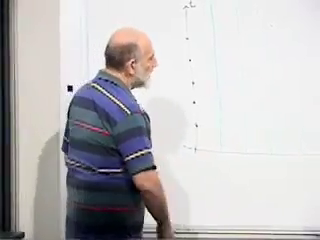
\includegraphics[width=0.62\textwidth]{lecture_01_figure_02.png}
\caption{정지계의 시간축과 공간 격자의 첫 세계선들.}
\lectureframe{00:16:38}
\end{figure}

같은 구성을 이상화한 그림으로 나타내면 더 분명하다.

\begin{figure}[H]
\centering
\begin{tikzpicture}[scale=0.95]
\draw[->] (-1.2,0) -- (5.2,0) node[right] {$x$};
\draw[->] (0,-0.2) -- (0,4.8) node[above] {$t$};
\foreach \x in {-1,1,2,3,4}
  \draw[gray!65] (\x,0) -- (\x,4.4);
\foreach \y in {1,2,3,4}
  \draw[gray!65] (-1.0,\y) -- (4.4,\y);
\fill (0,0) circle (1.5pt);
\node[below left] at (0,0) {$0$};
\node[left] at (0,1) {$1$};
\node[left] at (0,2) {$2$};
\node[left] at (0,3) {$3$};
\node[below] at (1,0) {$1$};
\node[below] at (2,0) {$2$};
\node[below] at (3,0) {$3$};
\end{tikzpicture}
\caption{정지한 시공간 격자. 수직선은 위치가 일정한 점들을, 수평선은 시간이 일정한 점들을 나타낸다.}
\end{figure}

격자는 상상 속의 것이며 간격은 임의로 정할 수 있다. 미터, 센티미터, 마이크론을 쓰거나 물리적으로 의미 있는 더 작은 간격을 쓸 수도 있다. 격자의 목적은 모든 사건에 정확한 좌표를 부여하는 것이다.

이제 ‘기준계’라는 말은 실제적인 의미를 갖는다. 단순히 어떤 방향을 바라보는 관점이나 사람을 가리키는 말이 아니다. 기준계는 공간 전체에 펼쳐진 좌표 장치다. 사건이 주어지면 그곳의 자가 어디서 일어났는지 알려 주고, 그곳의 시계가 언제 일어났는지 알려 준다. 그러면 입자의 위치와 속도, 에너지, 물체의 온도, 나아가 운동량과 힘 같은 다른 물리량도 기준계 사이에서 비교할 수 있다. 가장 간단한 비교는 \(x\)와 \(t\)에 관한 것이므로, 여기서부터 시작하자.

이제 일정한 속도 \(v\)로 양의 \(x\) 방향을 따라 움직이는 기차에 두 번째 격자를 놓자. 두 원점은 \(t=0\)에 일치하도록 정한다. 그러면 움직이는 원점의 궤적은 다음과 같다.
\begin{equation}
x=vt.
\end{equation}
기차에 고정된 다른 모든 점은 기울어진 평행 세계선을 따라간다. 이 기울기는 시간이 지남에 따라 기차의 위치가 변한다는 기하학적 표현일 뿐이다.

기차의 뒤쪽 끝이 프라임 원점이라고 하자. \(t=0\)에는 역의 원점과 일치한다. 그보다 뒤의 시각 \(t\)에는 역 기준 좌표가 \(vt\)이다. 따라서 좌표 \(x\)에 있는 인접한 사건은 기차 원점에서 \(x-vt\)만큼 떨어져 있다. 이것이 변환식이 임의의 대수 규칙이 아니라 뺄셈 형태인 이유다.

역 기준계에서 사건의 좌표를 \((x,t)\), 기차 기준계에서 그 좌표를 \((x',t')\)라 하자. 갈릴레이와 뉴턴은 보편적 시간을 그대로 유지한다.
\begin{equation}
t'=t.
\end{equation}
시간 \(t\) 동안 움직이는 원점은 \(vt\)만큼 전진하므로, 그 원점에서 사건까지의 거리는 다음과 같다.
\begin{equation}
x'=x-vt.
\end{equation}
두 식을 합치면,
\begin{align}
t'&=t, & x'&=x-vt.
\label{eq:galilean-forward}
\end{align}
미분 표시가 없는 좌표를 구하면 역변환은 다음과 같다.
\begin{align}
t&=t', & x&=x'+vt'.
\label{eq:galilean-inverse}
\end{align}

\begin{figure}[H]
\centering
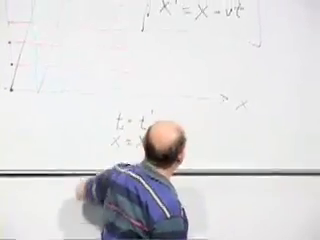
\includegraphics[width=0.72\textwidth]{lecture_01_figure_03.png}
\caption{두 시공간 격자 옆에 나타낸 갈릴레이 변환.}
\lectureframe{00:21:57}
\end{figure}

첫 번째 식은 움직이는 관찰자에게 정지한 관찰자가 준 좌표를 어떻게 변환할지 알려 준다. 역변환 쌍은 좌표를 다시 되돌린다. 두 기술 사이의 이 상호적인 변환이 갈릴레이 상대성의 수학적 내용이다.

역공간 변환식에서 \(t\to t'\)로 바꾸는 것은 갈릴레이 이론이 이미 \(t=t'\)라고 선언했기 때문에 문제가 없다. 이 가정을 지금 짚어 두는 것이 좋다. 아인슈타인 이론에서는 두 시간 좌표가 달라지므로, 이런 대입을 자동으로 할 수 없다.

\begin{classroomqa}
\audiencequestion{시계를 다른 곳으로 옮겼다가 다시 가져오면, 시계가 움직이는 동안 먼저 빨라졌다가 나중에 느려져 비교할 때 그 효과가 상쇄된 것은 아닌지 어떻게 알 수 있나요?
\lecturetimestamp{00:23:09}}
\lecturerresponse{갈릴레이는 오늘날의 정밀도로 보편적 시간을 확립할 수 없었다. 그것은 물리적 추측이었다. 좋은 시계를 서로 반대 방향으로 옮기거나, 동쪽--서쪽뿐 아니라 북쪽--남쪽으로도 이동을 반복하거나, 한 시계를 다른 시계 주위로 움직이거나, 시계를 한데 모으지 않은 채 시간 신호를 교환하는 등 여러 방법으로 이 추측을 시험할 수 있다. 일상적인 속도에서는 이런 시험이 모두 매우 높은 정밀도로 일치한다. 충분히 정밀한 시계나 충분히 큰 속도를 사용하면 작은 차이가 나타난다. 보편적 시간이 성립하지 않는다는 사실은 실험의 결함이 아니다. 이는 특수 상대성 이론이 설명해야 할 현상 중 하나다.}
\end{classroomqa}

\section{갈릴레이 불변량과 뉴턴 법칙}

불변량이란 논의 대상인 모든 관성계의 관찰자가 같은 값을 얻는 물리량이다. 좌표 자체가 불변일 필요는 없다. 중요한 것은 그 좌표로 세운 법칙이 같은 형태를 유지하는지 여부다.

이 말은 명사와 형용사로 모두 쓰인다. 수가 불변량일 수 있고, 방정식이 변환에 대해 불변일 수도 있다. 불변량과 불변 법칙을 구분하면 흔한 혼동을 피할 수 있다. 상대성 이론은 모든 관찰자가 모든 것에 대해 같은 좌표를 얻는다고 주장하지 않는다. 관측값 사이의 물리 법칙이 같은 형태를 갖는다고 주장한다.

위치 \(x_1\)와 \(x_2\)에 있는 두 사건이 동시에 일어난다고 하자. 식~\eqref{eq:galilean-forward}을 적용하면 다음과 같다.
\begin{align}
x_1'&=x_1-vt,\\
x_2'&=x_2-vt.
\end{align}
따라서 두 사건 사이의 거리는 다음과 같다.
\begin{equation}
x_2'-x_1'=(x_2-vt)-(x_1-vt)=x_2-x_1.
\end{equation}
갈릴레이 물리학에서는 같은 시각에 일어난 사건들 사이의 거리가 불변이다. 개별 위치는 불변이 아니더라도 그렇다.

\begin{classroomqa}
\audiencequestion{그 뺄셈에 나오는 \(t\)가 정말 같은 시각인가요?
\lecturetimestamp{00:28:16}}
\lecturerresponse{그렇다. 두 사건이 \((x_1,t)\)와 \((x_2,t)\)에 있도록 의도적으로 정했다. 두 사건은 하나의 수평 일정 시간선 위에 놓인다. 따라서 공통 항 \(vt\)은 소거된다. 사건들의 시각이 서로 달랐다면 이 논증으로 공간적 거리가 불변이라고 결론 내릴 수 없다.}
\end{classroomqa}

이제 입자의 궤적을 \(x(t)\)로 나타내자. 기차 안 관찰자는 다음과 같이 좌표를 정한다.
\begin{equation}
x'(t)=x(t)-vt.
\end{equation}
한 번 미분하면 익숙한 속도 합성 법칙이 나온다.
\begin{equation}
\frac{dx'}{dt}=\frac{dx}{dt}-v.
\end{equation}
위치와 속도는 기준계에 따라 달라진다. 화살을 나란히 따라 움직이는 관찰자는 선로 옆에 서 있는 관찰자보다 화살이 더 느리게 움직인다고 본다.

한 번 더 미분하자. 상대 속도 \(v\)는 일정하므로,
\begin{equation}
\frac{d^2x'}{dt^2}=\frac{d^2x}{dt^2}.
\end{equation}
가속도는 갈릴레이 변환 아래 불변이다. 뉴턴 법칙이 위치나 속도가 아니라 가속도로 쓰이는 이유가 여기에 있음을 알 수 있다.

여기서 말하는 것은 관찰 대상의 가속도이지, 기차 안 관찰자의 가속도가 아니다. 두 기준계는 관성계이므로 서로에 대해 가속하지 않는다. 어느 쪽 관점에서든 물체는 왼쪽이나 오른쪽으로 가속할 수 있다. 두 관찰자는 그 물체의 위치와 속도에는 동의하지 않지만 가속도 값에는 동의한다.

두 입자가 서로 힘을 미치고 그 힘이 두 입자 사이의 동시적 거리에만 의존한다고 하자. 그 거리는 불변이므로 힘도 불변이다. 질량 또한 물체에 고유하며 기준계와 무관한 성질이라면, 모든 관성계 관찰자는 다음을 쓸 수 있다.
\begin{equation}
F=ma
\end{equation}
그 형태는 완전히 동일하다. 뉴턴 역학은 갈릴레이 변환에 대해 불변이다. 이는 그럴듯한 주장에 그치지 않는다. 일상적인 속도의 영역에서 뉴턴 역학은 놀라울 정도로 정확하다.

이 논증은 거리의 함수로 크기가 정해지는 뉴턴 중력이나 정전기력 같은 익숙한 중심력에 적용된다. 모든 갈릴레이 관찰자는 같은 시각에 그 거리에 동의하므로 힘에도 동의한다. 힘과 가속도가 같다면 일관성을 위해 질량에도 동의해야 한다. 즉 기차가 지나가도 1킬로그램 물체는 여전히 1킬로그램이다. \(F=ma\)의 모든 기호는 같은 불변 구조를 따른다.

\section{빛에는 갈릴레이 법칙이 적용되지 않는다}

전자기학에서 문제가 생긴다. 맥스웰 방정식은 빈 공간을 일정한 속도 \(c\)로 이동하는 파동을 예측한다. 맥스웰 방정식이 자연 법칙이고 자연 법칙이 모든 관성계에서 동일하다면, 모든 관성계의 관찰자는 같은 \(c\)를 얻어야 한다.

갈릴레이 운동학은 다른 결과를 예측한다. 정지계에서 오른쪽으로 진행하는 빛 펄스는 다음을 만족한다.
\begin{equation}
x=ct.
\end{equation}
공간 변환을 적용하면,
\begin{equation}
x'=x-vt=(c-v)t.
\end{equation}
\(t'=t\)이므로 기차 안 관찰자는 속도를 \(c-v\)로 측정하게 된다.

모순은 명확하게 표현할 수 있다. 맥스웰 방정식의 형태가 유지된다면 프라임 기준계에서는 \(c\)를 예측한다. 갈릴레이 변환을 유지한다면 \(c-v\)를 예측한다. \(v\ne0\)일 때 두 결과가 모두 정확할 수는 없다.

빛이 매질 속에서 진행하는 보통의 파동처럼 행동한다고 보면 이 결과는 아주 자연스럽다. 물결과 함께 움직이는 배에서는 물결의 상대 속도가 더 낮게 측정된다. 정지한 공기 속을 움직이는 청자는 공기에 대한 자신의 운동에 따라 달라지는 음속을 측정한다. 따라서 19세기 물리학자들은 맥스웰 방정식이 가장 단순한 형태를 갖고 빛이 \(c\)로 움직이는, 우선적인 정지 상태인 에테르 기준계를 상정하게 되었다. 그러나 이 우선 기준계에 대한 운동을 검출하려고 설계한 실험에서는 그에 해당하는 효과가 발견되지 않았다.

가능한 실험 방법은 여럿이었지만, 모두 운동 상태나 방향이 서로 다른 관찰자들이 빛의 전파를 비교하는 것이 목적이었다. 어느 실험에서도 예상된 갈릴레이식 속도 이동은 나타나지 않았다. 이는 사소한 기술적 불편이 아니었다. 상대성 원리와 맥스웰 방정식, 그리고 물려받은 공간 및 시간 개념 중 무엇을 유지할지 선택해야 했다.

아인슈타인은 이 충돌을 더 직접적으로 다루었다. 젊은 시절 그는 빛의 파동을 뒤쫓는다고 상상했다. 빛을 따라잡을 수 있다면 진동하는 전자기파의 무늬가 공간에 정지한 것처럼 보일 테지만, 맥스웰 방정식은 그런 정지한 빛의 파동을 허용하지 않는다. 그는 맥스웰 이론과 상대성 원리를 근본 원리로 받아들이고, 좌표에 숨어 있는 가정을 다시 검토하기로 했다.

이 재구성은 두 가지 가정에 기초한다.
\begin{enumerate}
\item 물리 법칙은 모든 관성계에서 같은 형태를 갖는다.
\item 진공 속 빛의 속도 \(c\)는 모든 관성계에서 같다.
\end{enumerate}

두 번째 가정은 갈릴레이 변환과 양립할 수 없다. 속도 합성 법칙보다 더 근본적인 무언가가 바뀌어야 한다. 아인슈타인은 두 가정을 유지하고, 겉보기에는 무해한 갈릴레이 방정식 \(t'=t\)을 재검토하는 간결한 길을 택했다.

\section{멀리 떨어진 시계 동기화하기}

공간 거리는 자를 이용해 정할 수 있지만, 멀리 떨어진 시계에는 동기화 규약이 필요하다. 관찰자를 중심점에 두고 두 시계를 같은 거리만큼 떨어진 곳에 놓자. 양 끝 시계가 정해진 시각을 가리킬 때 각각 빛을 내보내게 한다. 두 빛이 중심점에 동시에 도착하면 양 끝 시계가 동기화되었다고 하자. 한쪽 빛이 먼저 도착하면 해당 시계를 조정하고 절차를 반복한다.

\emph{중점}이라는 말은 해당 기준계에 이미 놓인 자를 사용해 정의한다. 따라서 이 검정에는 서로 다른 두 요소가 들어 있다. 양 끝에서 같은 공간적 거리에 놓인 점이어야 하고, 신호의 도착 시각도 같아야 한다. 어느 한 요소도 생략할 수 없다. 격자 전체에서 이 절차를 반복하면 뉴턴이 그저 가정했던 수평 일정 시간선이 만들어진다.

이 정의에서 빛을 사용하는 이유는 가정에 따라 빛의 속도가 모든 관성계에서 같기 때문이다. 격자에서 이웃한 모든 시계 쌍에 이 절차를 적용하면 격자 전체에 동기화된 시계들이 배열된다.

이제 두 번째 격자가 첫 번째 격자 사이로 움직이게 하자. 움직이는 장치의 중점은 자체 기준계에서 움직이는 양 끝점의 한가운데에 계속 놓인다. 그러나 정지한 장치를 기준으로 보면 중점은 한쪽에서 다가오는 빛에 가까워지면서 다른 쪽 빛에서는 멀어진다. 정지한 시계 기준으로 동시에 방출된 빛은 움직이는 중점에 동시에 도착하지 않는다. 움직이는 관찰자도 같은 중점 및 빛 규칙을 적용하므로, 그 관찰자는 두 방출이 동시에 일어났다고 할 수 없다. 각 기준계는 자기 시계를 일관되게 동기화하지만, 두 동기화 결과는 서로 다르다.

이것은 빛의 유한한 이동 시간 때문에 생기는 착시가 아니다. 각 관찰자는 빛이 도착하는 데 시간이 걸린다는 점을 알고 있으며, 같은 속도 \(c\)를 사용해 이를 보정한다. 보정을 마친 뒤에도 두 관찰자가 동시 사건의 쌍으로 선택하는 멀리 떨어진 사건이 서로 다르므로 의견 차이가 남는다. 상대적인 것은 동시성의 겉모습만이 아니라 동시성 자체다.

\begin{classroomqa}
\audiencequestion{빛 대신 소리로 시계를 동기화하면 이 결론을 피할 수 있나요?
\lecturetimestamp{00:49:03}}
\lecturerresponse{공기가 정지한 기준계에서는 소리를 동기화 신호로 쓸 수 있지만, 측정되는 소리의 속도는 모든 관성계에서 같지 않다. 정지한 공기를 통과해 움직이는 개방된 기차는 소리를 전달하는 매질에 대해 움직이므로, 앞뒤 방향의 소리 신호는 대칭적으로 움직이지 않는다. 가정에 따르면 빛은 다르다. 어느 관찰자를 특별하게 만드는 검출 가능한 광학적 매질은 없다. 그러므로 우리는 빛을 사용하고 그 결과를 받아들인다.}
\end{classroomqa}

질적으로 어떤 의견 차이가 생기는지는 분명하다. 이제 움직이는 관찰자가 정확히 어떤 사건들을 동시라고 판단하는지 계산해 보자.

\section{빛 신호를 이용한 구성}

이 구성을 위해 다음과 같이 단위를 정하는 것이 편리하다.
\begin{equation}
c=1.
\end{equation}
그러면 거리 한 단위는 빛이 시간 한 단위 동안 이동하는 거리다. 예를 들어 초와 짝을 이루는 광초, 또는 년과 짝을 이루는 광년을 사용할 수 있다. 공간과 시간의 단위가 같아져 속도는 무차원이 되고, 빛은 그림에서 \(45^\circ\) 각도로 나타난다. 오른쪽으로 가는 빛은 다음을 만족한다.
\begin{equation}
x=t+d,
\end{equation}
왼쪽으로 가는 빛은 다음을 만족한다.
\begin{equation}
x=-t+d'.
\end{equation}
원점을 지나는 두 빛의 궤적은 각각 \(x=t\)와 \(x=-t\)이다. 빛보다 느린 물체의 시간꼴 궤적은 수직축에 더 가깝다. 가상의 초광속 궤적은 수평축에 더 가깝게 놓인다.

그림에서 각도는 이 단위를 선택한 뒤에야 의미가 있다. 미터와 초를 사용하면 빛은 일 초 동안 약 \(3\times10^8\)미터를 이동하므로 거의 수평으로 보일 것이다. 거리에 광초를 사용하면 가로축의 눈금이 조정되어 인과적 기하가 드러난다.

움직이는 격자에 있는 평행 세계선 세 개를 생각해 보자.
\begin{equation}
x=vt,\qquad x=vt+L,\qquad x=vt+2L.
\label{eq:moving-worldlines}
\end{equation}
가운데 세계선은 양 끝점 사이의 동시성을 검정하는 관찰자에 해당한다. 세 점 모두 등속 운동을 하며 프라임 기준계에서는 서로의 배치를 유지한다.

\begin{figure}[H]
\centering
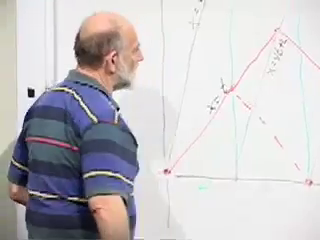
\includegraphics[width=0.72\textwidth]{lecture_01_figure_04.png}
\caption{가운데의 움직이는 세계선과 만나는 오른쪽 진행 빛 \(x=t\).}
\lectureframe{01:02:33}
\end{figure}

칠판 앞에 서 있는 사람이 가리지 않도록 전체 기하를 그려 보자.

\begin{figure}[H]
\centering
\begin{tikzpicture}[scale=0.95]
\draw[->] (-0.5,0) -- (6.5,0) node[right] {$x$};
\draw[->] (0,-0.2) -- (0,4.3) node[above] {$t$};
\draw[blue] (0,0) -- (1.4,4.0);
\draw[blue] (2.0,0) -- (3.4,4.0);
\draw[blue] (4.0,0) -- (5.4,4.0);
\draw[red] (0,0) -- (3.08,3.08);
\draw[red] (3.08,3.08) -- (4.56,1.60);
\draw[red,dashed] (2.0,0) -- (4.56,1.60);
\fill (0,0) circle (1.5pt);
\fill (2.0,0) circle (1.5pt);
\fill (4.0,0) circle (1.5pt);
\fill (3.08,3.08) circle (1.5pt);
\fill (4.56,1.60) circle (1.5pt);
\node[left] at (0.55,1.55) {$x=vt$};
\node[left] at (2.45,1.9) {$x=vt+L$};
\node[right] at (4.72,1.9) {$x=vt+2L$};
\node[left] at (1.88,2.28) {$x=t$};
\node[above right] at (3.08,3.08) {$A$};
\end{tikzpicture}
\caption{빛 신호가 움직이는 기준계의 동시성선을 정한다.}
\end{figure}

원점에서 오른쪽으로 가는 빛을 쏘자. \(A\)를 그 빛이 가운데 세계선과 만나는 사건이라고 하자. \(A\)에서 얻는 두 방정식은 다음과 같다.
\begin{align}
x&=t,\\
x&=vt+L.
\end{align}
대입하면 다음을 얻는다.
\begin{equation}
t=vt+L,
\end{equation}
따라서
\begin{equation}
t_A=x_A=\frac{L}{1-v}.
\label{eq:point-a}
\end{equation}

\(A\)에서 왼쪽으로 가는 빛을 따라 오른쪽 끝의 움직이는 세계선까지 거슬러 올라가자. 그 빛의 방정식은 다음 형태다.
\begin{equation}
x+t=b.
\end{equation}
이 빛은 \(A\)을 지나므로, 방정식~\eqref{eq:point-a}이 상수를 정해 준다.
\begin{equation}
b=x_A+t_A=\frac{2L}{1-v}.
\end{equation}
따라서 역방향 빛의 식은 다음과 같다.
\begin{equation}
x+t=\frac{2L}{1-v}.
\label{eq:backward-ray}
\end{equation}

오른쪽 끝 세계선과의 교점은 다음 두 식으로 구할 수 있다.
\begin{align}
x+t&=\frac{2L}{1-v},\\
x&=vt+2L.
\end{align}
\(x\)를 소거하면,
\begin{align}
(1+v)t
  &=2L\left(\frac{1}{1-v}-1\right)\\
  &=\frac{2Lv}{1-v},
\end{align}
따라서
\begin{equation}
t=\frac{2Lv}{1-v^2}.
\end{equation}
이를 \(x=vt+2L\)에 대입하면,
\begin{equation}
x=\frac{2L}{1-v^2}.
\end{equation}
좌표값 자체보다 두 좌표의 비가 중요하다.
\begin{equation}
\frac{t}{x}=v.
\end{equation}
그러므로 움직이는 시계 기준으로 원점과 동시에 일어나는 모든 사건은 다음 직선 위에 놓인다.
\begin{equation}
t=vx,
\label{eq:simultaneity-c-one}
\end{equation}
반면 움직이는 원점은 다음을 따른다.
\begin{equation}
x=vt.
\label{eq:moving-time-axis}
\end{equation}
두 축은 \(45^\circ\) 빛을 기준으로 대칭되게 기울어져 있다.

\(x=vt\) 위의 모든 점은 같은 프라임 위치 \(x'=0\)를 갖지만 프라임 시각은 달라진다. \(t=vx\) 위의 모든 점은 같은 프라임 시각 \(t'=0\)을 갖지만 프라임 위치는 달라진다. 따라서 한 직선은 프라임 시간축이고 다른 직선은 프라임 공간축이다. 두 번째 직선을 정하려면 긴 신호 구성이 필요했다. 움직이는 세계선만으로는 이를 추론할 수 없었다.

방정식~\eqref{eq:simultaneity-c-one}에 일반적인 단위를 복원하려면 다음이 필요하다.
\begin{equation}
t=\frac{v}{c^2}x.
\label{eq:simultaneity-dimensional}
\end{equation}
인자 \(c^2\)는 뉴턴적 그림이 일상생활에서 잘 들어맞는 이유를 설명한다. 속도가 \(c\)에 비해 아주 작으면 움직이는 동시성선의 기울기는 극히 작다.

\begin{figure}[H]
\centering
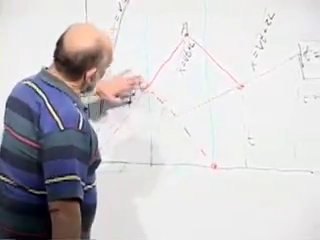
\includegraphics[width=0.72\textwidth]{lecture_01_figure_05.png}
\caption{\(c=1\)일 때 프라임 시간축과 동시성축은 빛을 기준으로 대칭이다.}
\lectureframe{01:15:40}
\end{figure}

\begin{figure}[H]
\centering
\begin{tikzpicture}[scale=1.0]
\draw[->] (-2.2,0) -- (5.2,0) node[right] {$x$};
\draw[->] (0,-0.2) -- (0,4.9) node[above] {$t$};
\draw[red] (0,0) -- (3.9,3.9);
\draw[red] (0,0) -- (-1.8,1.8);
\draw[blue] (0,0) -- (1.8,4.5);
\draw[blue,dashed] (0,0) -- (4.5,1.8);
\node[right] at (3.9,3.9) {$x=t$};
\node[left] at (-1.8,1.8) {$x=-t$};
\node[above] at (1.8,4.5) {$x'=0$};
\node[right] at (4.5,1.8) {$t'=0$};
\end{tikzpicture}
\caption{\(c=1\) 단위에서 프라임 축과 불변인 빛의 궤적.}
\end{figure}

\section{로런츠 변환 유도}

기하를 통해 각 프라임 좌표가 어디에서 영이 되는지 알 수 있다. 움직이는 시간축 \(x=vt\)에서는 \(x'=0\)이어야 한다. 움직이는 동시성축 \(t=vx\)에서는 \(t'=0\)이어야 한다. 이 영점 조건을 만족하는 가장 일반적인 선형 관계는 다음과 같이 쓸 수 있다.
\begin{align}
x'&=\frac{x-vt}{F(v)},\\
t'&=\frac{t-vx}{G(v)}.
\label{eq:fg-ansatz}
\end{align}
인자 \(F\)와 \(G\)는 축의 위치가 이미 정해졌더라도 프라임 좌표의 눈금이 갈릴레이식 눈금과 다를 수 있게 한다. 공간과 시간의 균질성으로부터 선형성이 따른다. 즉 실험을 평행 이동해도 변환 법칙은 달라지지 않는다.\editorialnote{이 짧은 선형성 논증은 칠판에서 유도할 때 암묵적으로 사용한 가정을 분명하게 드러낸다.}

이 단계에서 기하는 많은 것을 알려 주었지만 전부 알려 주지는 않았다. 분자는 축의 기울기를 정한다. 하지만 축을 따라 단위 간격이 어떻게 정해지는지는 알려 주지 않는다. 남은 눈금 정보가 바로 \(F(v)\)와 \(G(v)\)가 나타내는 것이다.

이제 빛의 속도가 불변이라는 조건을 부과하자. \(x=t\)를 따르는 오른쪽 진행 빛은 \(x'=t'\)도 만족해야 한다. 그 빛을 따라가면,
\begin{align}
x'&=\frac{(1-v)t}{F(v)},\\
t'&=\frac{(1-v)t}{G(v)}.
\end{align}
빛 궤적의 모든 점에서 이 관계가 성립하려면,
\begin{equation}
F(v)=G(v).
\end{equation}
따라서 다음과 같이 쓸 수 있다.
\begin{align}
x'&=\frac{x-vt}{F(v)},\\
t'&=\frac{t-vx}{F(v)}.
\label{eq:common-f}
\end{align}

이 단계에서는 대수적으로 처음으로 아인슈타인다운 요구 조건을 사용한다. 두 관찰자 모두에게 같은 기하학적 직선이 빛의 궤적이므로, \(c=1\)일 때 두 프라임 좌표는 그 선을 따라 똑같이 증가해야 한다. 두 식의 인자가 다르면 프라임 기준계에서 빛의 속도는 단위값과 달라진다.

미지 함수가 하나 남았다. 방정식~\eqref{eq:common-f}에 \(F(v)\)를 곱하면,
\begin{align}
F(v)x'&=x-vt,\\
F(v)t'&=t-vx.
\end{align}
두 번째 방정식에 \(v\)를 곱하고 첫 번째 식에 더하면 \(t\)가 소거되어 다음을 얻는다.
\begin{equation}
(1-v^2)x=F(v)(x'+vt').
\end{equation}
마찬가지로,
\begin{equation}
(1-v^2)t=F(v)(t'+vx').
\end{equation}
따라서 역변환은 다음과 같다.
\begin{align}
x&=\frac{F(v)}{1-v^2}(x'+vt'),\\
t&=\frac{F(v)}{1-v^2}(t'+vx').
\end{align}

상대성 원리에 따라 두 기준계는 서로 대칭적이다. 역에서는 기차가 \(+v\)로 움직이는 것으로 보인다면, 기차에서는 역이 \(-v\)로 움직이는 것으로 보인다. 따라서 역방정식은 \(v\)의 부호를 바꾼 같은 형태를 가져야 한다. 두 식의 앞 인자는 다음 조건을 만족해야 한다.
\begin{equation}
\frac{F(v)}{1-v^2}=\frac{1}{F(v)}.
\end{equation}
그러므로
\begin{equation}
F(v)^2=1-v^2,
\end{equation}
그리고 \(v=0\)에서 항등 변환과 연속이어야 하므로 양의 근을 택한다.
\begin{equation}
F(v)=\sqrt{1-v^2}.
\end{equation}

이 결과는 특정한 빛 펄스에 맞춰 조정한 것이 아니다. 동기화로 정해진 축, 빛의 공통 속도, 어느 관성계도 다른 관성계보다 우선하지 않는다는 요구에서 나온다.

\(c=1\)인 단위계에서 로런츠 변환은 다음과 같다.
\begin{align}
x'&=\frac{x-vt}{\sqrt{1-v^2}},\\
t'&=\frac{t-vx}{\sqrt{1-v^2}}.
\label{eq:lorentz-c-one}
\end{align}
역변환은 다음과 같다.
\begin{align}
x&=\frac{x'+vt'}{\sqrt{1-v^2}},\\
t&=\frac{t'+vx'}{\sqrt{1-v^2}}.
\end{align}

\begin{figure}[H]
\centering
\includegraphics[width=0.76\textwidth]{lecture_01_figure_06.png}
\caption{완성된 \(c=1\) 로런츠 변환을 칠판에 나타낸 모습.}
\lectureframe{01:32:38}
\end{figure}

핵심적인 새로움은 시간 방정식에 이미 드러나 있다. 시간은 한 기준계에서 다른 기준계로 그대로 옮겨지지 않는다. 프라임 시간 좌표에는 프라임이 없는 시간과 위치가 섞인다. 따라서 \(t=\text{constant}\)와 \(t'=\text{constant}\)는 서로 다른 사건 집합을 나타낸다.

이 혼합 항은 나중에 덧붙이는 선택적 보정 항이 아니다. 이 항이 없으면 \(t'=0\) 직선은 수평으로 남고, 멀리 떨어진 곳 사이의 동시성은 보편적인 채로 유지되며, 변환은 빛의 속도를 보존할 수 없다.

\section{빛의 속도 복원과 결과 검산}

\(c\ne1\)이면 차원 일관성을 위해 빠진 인자들을 복원해야 한다. 비 \(v^2/c^2\)는 무차원이고 \((v/c^2)x\)는 시간의 단위를 갖는다. 따라서
\begin{align}
x'&=\frac{x-vt}{\sqrt{1-v^2/c^2}},\\
t'&=\frac{t-(v/c^2)x}{\sqrt{1-v^2/c^2}}.
\label{eq:lorentz-dimensional}
\end{align}
\(v\)의 부호를 바꾸면 역변환을 얻는다.
\begin{align}
x&=\frac{x'+vt'}{\sqrt{1-v^2/c^2}},\\
t&=\frac{t'+(v/c^2)x'}{\sqrt{1-v^2/c^2}}.
\end{align}
다음을 도입하면,
\begin{equation}
\gamma=\frac{1}{\sqrt{1-v^2/c^2}}
\end{equation}
식은 익숙한 간결한 형태로 쓸 수 있지만, 분모 형태를 유지하면 유도 과정을 확인하기 쉽다.

수치로는 \(c\simeq3\times10^8\,\mathrm{m/s}\)이므로 \(c^2\simeq9\times10^{16}\,\mathrm{m^2/s^2}\)이다. 분모가 크기 때문에 대부분의 역학 실험에서는 동시성선의 기울기와 인자 \(v^2/c^2\)를 감지할 수 없다. 이 효과가 작은 덕분에 갈릴레이 역학이 성공했지만, 절대 시간이 되살아나는 것은 아니다.

\begin{figure}[H]
\centering
\includegraphics[width=0.76\textwidth]{lecture_01_figure_07.png}
\caption{인자 \(c\)를 복원한 로런츠 변환.}
\lectureframe{01:35:58}
\end{figure}

두 가지 점검을 바로 할 수 있다. 먼저 \(v\ll c\)로 두자. 그러면 \(v^2/c^2\)은 무시할 수 있고, 보통의 거리에서는 동시성의 상대성에 따른 항 \(vx/c^2\)도 무시할 수 있다. 식~\eqref{eq:lorentz-dimensional}은 다음과 같이 된다.
\begin{equation}
t'\approx t,\qquad x'\approx x-vt.
\end{equation}
저속 근사에서 갈릴레이 상대성이 회복된다.

둘째, 광선을 살펴보자. \(c\)를 다시 넣으면 오른쪽으로 진행하는 광선은 \(x=ct\)을 따르며, \(x=t\)을 따르지 않는다. 이를 대입하면 다음을 얻는다.
\begin{align}
x'&=\frac{(c-v)t}{\sqrt{1-v^2/c^2}},\\
t'&=\frac{(1-v/c)t}{\sqrt{1-v^2/c^2}}.
\end{align}
\(c-v=c(1-v/c)\)이므로,
\begin{equation}
x'=ct'.
\end{equation}
프라임 좌표계의 관측자도 같은 속력 \(c\)을 측정한다. 왼쪽으로 진행하는 광선에 \(x=-ct\)를 대입해도 마찬가지로 다음을 얻는다.
\begin{equation}
x'=-ct'.
\end{equation}
이 변환은 어느 방향으로 진행하는 빛에도 올바르게 적용된다.

\(x=t\)와 \(x=ct\)의 차이는 차원을 확인하는 데 유용하다. 전자는 \(c=1\)인 단위계에서만 옳다. 광선 방정식은 자연 단위계에 둔 채 변환식에만 보통 단위를 다시 넣으면 두 단위 관례가 뒤섞여 잘못된 결과가 나온다. 차원의 일관성을 확인하면 이 실수를 바로 알아낼 수 있다.

\section{중점 기준}

\begin{classroomqa}
\audiencequestion{관측자가 두 광원에서 나온 섬광을 동시에 받았지만 두 광원의 중간 지점에 있지는 않다고 하자. 이 관측자는 두 섬광이 동시에 방출되었다고 결론 내릴 수 있는가?
\lecturetimestamp{01:42:55}}
\lecturerresponse{아니다. 도착 시간이 같다는 사실로 방출 시간도 같다고 결론 내릴 수 있는 것은 관련 좌표계에서 두 광원의 공간적 중간에 있는 관측자뿐이다. 한 광원에 더 가까운 수신자는 더 먼 쪽의 섬광이 먼저 방출되었는데도 두 섬광을 동시에 받을 수 있다. 따라서 움직이는 구성에서는 중점 세계선 \(x=vt+L\)이 필수적이다. 정방향 광선 \(x=t\)을 그 중점에 닿을 때까지 따라간 뒤, 역방향 광선을 \(x=vt+2L\)까지 거슬러 추적한다. 그 두 번째 끝점 사건은 다른 곳에서 임의로 택한 도착 동시 사건이 아니라, 움직이는 좌표계에서 원점과 동시인 사건이다.}
\end{classroomqa}

좌표 변환 전체를 얻었지만, 이제 가장 익숙한 결과들을 살펴볼 차례다. 다음으로 길이 수축, 시간 지연, 고유 시간을 다루고, 이어서 상대론적 운동량과 에너지를 다룬다. 토대는 이미 마련되었다. 각 관성계가 같은 법칙을 쓰고 같은 빛의 속력을 측정할 수 있는 것은 공간과 시간이 서로 섞이고, 멀리 떨어진 사건의 동시성이 절대적으로 정해지는 것이 아니라 좌표계에 속하기 때문이다.

\chapter{맥스웰 방정식, 공변성, 그리고 전자기파}

\lectureoverview{전기장과 자기장은 로런츠 힘을 통해 하전 물질에 작용하지만, 물질도 전기장과 자기장을 만들어 재배열해야 합니다. 이번에는 전자기학의 이 상호적인 나머지 절반을 정식화하고, 맥스웰 방정식이 로런츠 공변임을 보이며, 파동 해를 유도한 다음, 국소 보존이 명확히 드러나는 형태로 전하와 전류를 다시 포함하겠습니다. 강의 전체에서 \(c=1\)인 단위를 사용합니다.}

\section{전자기학의 다른 절반}

먼저 이미 살펴본 부분부터 시작합시다. 전하 \(q\)인 입자가 전기장과 자기장 속에서 속도 \(\mathbf v\)로 움직이면, 힘은 다음과 같습니다.
\begin{equation}
\mathbf F=q\bigl(\mathbf E+\mathbf v\times\mathbf B\bigr).
\label{eq:lorentz-force-three}
\end{equation}
인자 \(q\)는 반드시 필요합니다. 전하가 없는 입자는 전자기력을 느끼지 않습니다. 입자가 순간적으로 정지해 있어도 전기장은 힘에 기여하지만, 자기장의 기여는 입자의 운동에 달려 있습니다.

방정식~\eqref{eq:lorentz-force-three}은 주어진 장이 물질에 어떤 작용을 하는지 알려 줍니다. 하지만 장을 결정하는 것이 무엇인지는 말해 주지 않습니다. 한 물체 주위의 전기장, 다른 물체 주위의 자기장, 또는 빈 공간을 따라 움직이는 파동은 무엇이 만들어 낼까요? 이 질문에 답하는 방정식이 맥스웰 방정식입니다.

\begin{figure}[H]
\centering
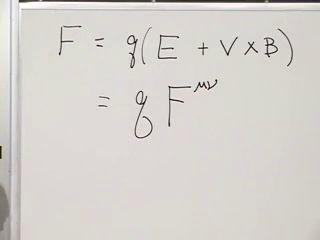
\includegraphics[width=0.62\textwidth]{lecture_58_figure_02.png}
\caption{3차원 로런츠 힘과 그 텐서 표현의 시작.}
\lectureframe{00:05:49}
\end{figure}

힘 법칙의 상대론적 형태에는 앞으로 필요한 표기법이 이미 담겨 있습니다.
\begin{equation}
f^\mu=qF^\mu{}_{\nu}u^\nu.
\label{eq:lorentz-force-four}
\end{equation}
여기서 \(u^\nu\)는 4-속도, \(f^\mu\)는 4-힘이며, \(F^{\mu\nu}\)는 \(\mathbf E\)와 \(\mathbf B\)로 구성한 반대칭 텐서입니다. 판서에는 우선 이 식의 개략적인 시작 부분만 나타나 있습니다. \(u^\nu\)와의 축약으로 빠져 있던 벡터가 더해져, 힘의 지표 하나가 자유 지표로 남습니다.

물질이 장에 다시 영향을 미쳐야 하는 데에는 물리적인 이유가 있습니다. 전자기파가 전하에 부딪히면 전하를 가속하고 에너지를 전달할 수 있습니다. 장은 전하에 영향을 주면서 전하는 장에 영향을 줄 수 없다면, 그 에너지가 어디서 빠져나오는지 설명할 길이 없습니다. 작용과 반작용만으로 논증이 끝나는 것은 아니지만, 에너지 보존을 생각하면 상호적인 결합은 불가피합니다.

\section{변화하는 원천은 교란을 내보낸다}

점전하는 그 위치에서 바깥쪽이나 안쪽을 향하는 전기장을 만듭니다. 도선의 전류--하전 입자들의 흐름--는 도선을 둘러싸고 회전하는 자기장을 만듭니다. 익숙한 이 정전기적·정자기적 그림만으로도 서로 다른 두 기하학적 형태를 볼 수 있습니다. 전기 플럭스는 전하에서 뻗어 나오고, 자기력선은 전류 주위를 감쌉니다.

이제 점전하를 갑자기 움직여 봅시다. 새 위치 근처에서는 전기장이 재배열되기 시작해야 하지만, 멀리 있는 관찰자는 그 움직임을 즉시 알 수 없습니다. 신호가 도달할 시간이 흐를 때까지 먼 곳에는 이전 장이 그대로 남습니다. 가까운 영역과 먼 영역 사이에는 장이 변하는 경계면이 이동합니다. 이렇게 이동하는 장의 재배열이 전자기 교란입니다.

전하를 왕복 운동시키면 재배열이 잇따라 일어나 전자기파를 이룹니다. 이것이 안테나의 기본 작동 원리입니다. 진동하는 전류가 장의 교란을 바깥으로 내보냅니다. 도선의 전류 방향을 뒤집어도 같은 논리로 자기장에 관한 그림을 얻습니다. \(\mathbf B\)의 회전 방향도 바뀌어야 하지만, 그 변화는 모든 곳에서 한꺼번에 나타나는 것이 아니라 전파됩니다.

이 인과적 그림은 맥스웰 방정식에 두 가지 조건을 요구합니다. 전하와 전류가 장의 원천이 되는 방식을 설명해야 하고, 장의 변화가 빛보다 빠르지 않게 전파될 수 있어야 합니다. 두 번째 조건은 상대성 이론을 검증하는 기준이기도 합니다. 맥스웰 방정식이 모든 관성계에서 같은 형태를 가지며 특정한 파동 속도를 함의한다면, 모든 관성계의 관찰자는 그 방정식에서 같은 속도를 얻어야 합니다.

\section{상대론적 파동 방정식 복습}

벡터장을 살펴보기 전에 스칼라장 \(\phi(\mathbf x,t)\)을 생각해 보자. 이는 시공간의 각 점에 하나의 수가 대응하는 장이다. 일계 미분 방정식
\begin{equation}
\partial_\mu\phi=0
\end{equation}
은 시공간의 모든 미분이 사라진다는 뜻이다. 그러면 장은 상수가 되어 파동을 전달할 수 없다. 비자명한 상대론적 파동 방정식에는 두 번의 미분이 들어간다.
\begin{equation}
\partial_\mu\partial^\mu\phi=0.
\end{equation}
여기서 사용한 부호 규약에 따르면
\begin{equation}
\left(\partial_t^2-\partial_x^2-\partial_y^2-\partial_z^2\right)\phi=0,
\label{eq:scalar-wave-four}
\end{equation}
또는 더 간결하게
\begin{equation}
\left(\partial_t^2-\nabla^2\right)\phi=0.
\end{equation}
이다. \(c=1\)로 두면 시간과 거리를 서로 양립하는 단위로 나타낼 수 있다. 일반적인 단위를 복원하면 시간에 대한 이계 미분항 옆에 \(1/c^2\)가 붙는다.

\(z\)축을 따라 진행하는 파동에서는 장이 \(z\)와 \(t\)에 의존하고, \(x\)나 \(y\)에는 의존하지 않습니다. 방정식~\eqref{eq:scalar-wave-four}은 다음과 같이 됩니다.
\begin{equation}
\left(\partial_t^2-\partial_z^2\right)\phi=0.
\label{eq:scalar-wave-one}
\end{equation}

\begin{figure}[H]
\centering
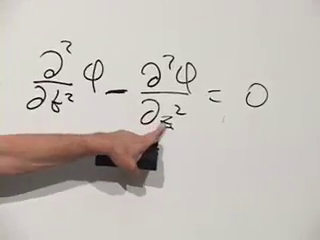
\includegraphics[width=0.56\textwidth]{lecture_58_figure_04.png}
\caption{전자기파의 모형으로 사용하는 1차원 스칼라 파동 방정식.}
\lectureframe{00:47:03}
\end{figure}

일반적인 진행파 해는 다음과 같습니다.
\begin{equation}
\phi(z,t)=f(z-t)+g(z+t).
\end{equation}
파형 \(f(z-t)\)은 위상이 일정한 점이 \(z-t=\text{constant}\)를 만족하므로 \(z\)가 증가하는 방향으로 이동합니다. 파형 \(g(z+t)\)은 반대 방향으로 이동합니다. 어느 파형도 정현파일 필요는 없습니다. 충분히 매끄러운 형태라면 모양을 바꾸지 않고 그대로 이동합니다.

그렇지만 정현파를 사용하면 편리합니다.
\begin{equation}
\phi(z,t)=A\cos\!\bigl(k(z-t)\bigr).
\end{equation}
파수 \(k\)는 파장을 결정합니다.
\begin{equation}
\lambda=\frac{2\pi}{k}.
\end{equation}
\(k\)가 크면 공간적으로 빠르게 진동하고 파장이 짧아집니다. \(k\)가 작으면 파장이 길어집니다. 곧 이 파형들은 \(\mathbf E\)와 \(\mathbf B\)의 성분이 됩니다.

\section{맥스웰 방정식에 필요한 벡터 미적분}

맥스웰 방정식에는 내적, 외적, 발산, 회전이 등장합니다. 뒤에서 성분별 계산에 바로 이 형태들을 사용하므로, 표기법을 한 번 다시 정리해 두겠습니다.

일반적인 3차원 벡터 \(\mathbf a\)와 \(\mathbf b\)에 대해 내적은 스칼라입니다.
\begin{equation}
\mathbf a\cdot\mathbf b
=a_xb_x+a_yb_y+a_zb_z.
\end{equation}
외적은 또 다른 벡터입니다.
\begin{align}
(\mathbf a\times\mathbf b)_x&=a_yb_z-a_zb_y,\\
(\mathbf a\times\mathbf b)_y&=a_zb_x-a_xb_z,\\
(\mathbf a\times\mathbf b)_z&=a_xb_y-a_yb_x.
\end{align}
나머지 성분은 순환 순서 \(x\to y\to z\to x\)에 따라 얻습니다.

미분 연산자
\begin{equation}
\boldsymbol\nabla=
\left(\partial_x,\partial_y,\partial_z\right).
\end{equation}
를 도입합시다. 각 성분은 보통 수가 아니라 연산자이지만, 내적과 외적의 형태를 그대로 사용할 수 있습니다. 벡터장 \(\mathbf A\)에 대해,
\begin{equation}
\boldsymbol\nabla\cdot\mathbf A
=\partial_xA_x+\partial_yA_y+\partial_zA_z
\label{eq:divergence}
\end{equation}
은 발산이고,
\begin{align}
(\boldsymbol\nabla\times\mathbf A)_x
 &=\partial_yA_z-\partial_zA_y,\\
(\boldsymbol\nabla\times\mathbf A)_y
 &=\partial_zA_x-\partial_xA_z,\\
(\boldsymbol\nabla\times\mathbf A)_z
 &=\partial_xA_y-\partial_yA_x
\label{eq:curl}
\end{align}
은 회전의 성분입니다.

기하학적 의미는 수식만큼이나 중요합니다. 벡터장이 원천으로부터 바깥쪽으로 흘러나오는 듯한 곳에서는 발산이 양수입니다. 벡터장이 회전하는 곳에는 회전이 있습니다. 점전하의 방사형 전기장은 발산을, 전류가 흐르는 도선을 감싸는 자기장은 회전을 보여 줍니다. 공간적으로 일정한 벡터장에는 둘 다 없습니다.

\section{진공에서의 맥스웰 방정식}

전하와 전류가 없을 때 맥스웰 방정식은 다음과 같습니다.
\begin{align}
\boldsymbol\nabla\times\mathbf E&=-\partial_t\mathbf B,
\label{eq:faraday-vac}\\
\boldsymbol\nabla\cdot\mathbf B&=0,
\label{eq:gauss-b-vac}\\
\boldsymbol\nabla\times\mathbf B&=\partial_t\mathbf E,
\label{eq:ampere-vac}\\
\boldsymbol\nabla\cdot\mathbf E&=0.
\label{eq:gauss-e-vac}
\end{align}
두 회전 방정식은 \(\mathbf E\)와 \(\mathbf B\)를 거의 맞바꾼 형태지만, 중요한 마이너스 부호 하나가 둘을 구별합니다. 두 발산 방정식은 고려하는 진공 영역에 어느 장에도 원천이 없음을 말합니다. 전기 원천을 다시 포함해도 자기장의 발산은 여전히 0입니다. 일반적인 전자기학에는 자기 전하가 없습니다.

\begin{figure}[H]
\centering
\includegraphics[width=0.76\textwidth]{lecture_58_figure_06.png}
\caption{전기장과 자기장 사이의 거의 대칭적인 관계가 드러나도록 배열한 진공 맥스웰 방정식 네 개.}
\lectureframe{00:27:30}
\end{figure}

전하 밀도 \(\rho\)는 결국 방정식~\eqref{eq:gauss-e-vac}의 우변에 있는 0을 대신하고, 전류 밀도 \(\mathbf J\)는 방정식~\eqref{eq:ampere-vac}에 들어갑니다. 잠시 이 항들을 미뤄 두겠습니다. 원천이 없는 방정식은 복잡한 항을 최소화한 채 변환 구조와 파동이 생기는 원리를 드러냅니다.

이 방정식들은 아인슈타인의 문제도 한층 선명하게 보여 줍니다. 파동을 따라 움직이는 갈릴레이 관찰자라면 속도를 빼서 파동 속도가 더 작게 측정될 것이라고 예상할 것입니다. 하지만 같은 맥스웰 방정식이 모든 관성계에서 성립한다면, 각 관찰자는 그 방정식에서 동일한 단위 파동 속도를 얻습니다. 해결책은 관성계마다 파동 방정식을 바꾸는 것이 아닙니다. 로런츠 변환을 사용하고, 변환 법칙이 이미 알려진 대상들로 맥스웰 방정식을 나타내는 것입니다.

\section{하나의 텐서로 묶이는 전기장과 자기장}

전기장과 자기장을 반대칭 장 텐서로 결합하면 다음과 같다.
\begin{equation}
F^{\mu\nu}=
\begin{pmatrix}
0   & -E_x & -E_y & -E_z\\
E_x & 0    & -B_z & B_y\\
E_y & B_z  & 0    & -B_x\\
E_z & -B_y & B_x  & 0
\end{pmatrix},
\label{eq:l0203-field-tensor}
\end{equation}
행과 열의 순서는 \(t,x,y,z\)이다. 반대칭성
\begin{equation}
F^{\mu\nu}=-F^{\nu\mu},
\end{equation}
에 의해 대각 성분은 영이 되고, 행렬의 아래쪽 절반은 위쪽 절반으로 결정된다. 시간과 공간에 해당하는 성분에는 \(\mathbf E\)가 들어가며, 공간에만 해당하는 성분에는 \(\mathbf B\)가 들어간다.

\begin{figure}[H]
\centering
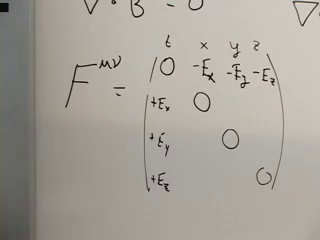
\includegraphics[width=0.58\textwidth]{lecture_58_figure_03.png}
\caption{전기장과 자기장 성분을 모두 포함한 완성된 전자기장 텐서.}
\lectureframe{00:32:05}
\end{figure}

\(F^{\mu\nu}\)가 중요한 이유는 장 성분 여섯 개를 하나의 행렬에 넣을 수 있다는 데 그치지 않습니다. 로런츠 변환 아래에서 이 텐서는 2계 텐서로 변환됩니다. 따라서 관찰자마다 측정하는 전기장과 자기장은 전체 텐서가 일관되게 변환되는 데 필요한 방식으로 서로 섞입니다.

또 다른 반대칭 텐서인 쌍대 장 텐서 \(\widetilde F^{\mu\nu}\)도 있습니다. 현재의 규약에서는 방정식~\eqref{eq:l0203-field-tensor}에 다음 치환을 적용해 얻습니다.
\begin{equation}
\mathbf E\longmapsto-\mathbf B,
\qquad
\mathbf B\longmapsto\mathbf E.
\label{eq:dual-replacement}
\end{equation}
따라서
\begin{equation}
\widetilde F^{\mu\nu}=
\begin{pmatrix}
0    & B_x  & B_y  & B_z\\
-B_x & 0    & -E_z & E_y\\
-B_y & E_z  & 0    & -E_x\\
-B_z & -E_y & E_x  & 0
\end{pmatrix}.
\label{eq:dual-tensor}
\end{equation}
방정식~\eqref{eq:dual-replacement}의 부호는 중요합니다. 강의에서는 먼저 말로 두 장을 맞바꾸어 보다가 부호가 맞지 않음을 알아차리고, 행렬을 완성하기 전에 이를 바로잡습니다.

\begin{figure}[H]
\centering
\includegraphics[width=0.58\textwidth]{lecture_58_figure_07.png}
\caption{필요한 부호를 포함해 전기장과 자기장 성분을 교환하며 구성하는 쌍대 텐서.}
\lectureframe{00:35:45}
\end{figure}

\section{공변적인 진공 방정식}

맥스웰 방정식은 각각 미분 하나를 포함합니다. 2계 텐서에서 한 미분 지표를 축약하면 자유 지표 하나가 남으므로, 공변적인 형태로 자연스럽게 생각할 수 있는 식은 다음과 같습니다.
\begin{align}
\partial_\mu F^{\mu\nu}&=0,
\label{eq:maxwell-covariant-vac}\\
\partial_\mu\widetilde F^{\mu\nu}&=0.
\label{eq:maxwell-dual-vac}
\end{align}
\(\nu\)를 하나의 고정된 값으로 두면 방정식~\eqref{eq:maxwell-covariant-vac}은 하나의 방정식입니다. \(\nu\)는 \(t,x,y,z\) 가운데 하나일 수 있으므로, 이 식은 스칼라 방정식 네 개를 묶습니다. 방정식~\eqref{eq:maxwell-dual-vac}은 나머지 네 개를 묶습니다. 이는 앞서 나열한 벡터 회전 방정식 두 개와 스칼라 발산 방정식 두 개에 해당합니다.

간결한 표기는 익숙한 방정식을 재현할 때만 유용하다. \(\nu=z\)으로 두면
\begin{align}
\partial_\mu F^{\mu z}
&=\partial_tF^{tz}
  +\partial_xF^{xz}
  +\partial_yF^{yz}
  +\partial_zF^{zz}\\
&=-\partial_tE_z+\partial_xB_y-\partial_yB_x\\
&=-\partial_tE_z+
  \bigl(\boldsymbol\nabla\times\mathbf B\bigr)_z.
\end{align}
항 \(F^{zz}\)는 반대칭성 때문에 영이 된다. 결과를 영으로 놓으면 \(z\) 성분에 해당하는 다음 식을 얻는다.
\begin{equation}
\boldsymbol\nabla\times\mathbf B=\partial_t\mathbf E.
\end{equation}
지표를 순환시키면 \(x\) 및 \(y\) 성분도 얻어진다.

\begin{figure}[H]
\centering
\includegraphics[width=0.76\textwidth]{lecture_58_figure_08.png}
\caption{공변 장 방정식을 성분별로 전개하면, 대각 텐서 성분은 사라지고 나머지 항들이 맥스웰 방정식을 재구성한다.}
\lectureframe{00:43:30}
\end{figure}

이제 시간 성분을 살펴봅시다.
\begin{align}
\partial_\mu F^{\mu t}
&=\partial_tF^{tt}
  +\partial_xF^{xt}
  +\partial_yF^{yt}
  +\partial_zF^{zt}\\
&=\partial_xE_x+\partial_yE_y+\partial_zE_z\\
&=\boldsymbol\nabla\cdot\mathbf E.
\end{align}
따라서 방정식~\eqref{eq:gauss-e-vac}을 줍니다. 쌍대 텐서에 대해서도 같은 검산을 하면
\(\boldsymbol\nabla\cdot\mathbf B=0\)와
\(\boldsymbol\nabla\times\mathbf E=-\partial_t\mathbf B\)를 얻습니다.

이제 간결한 방정식들은 단순히 추측한 것이 아니라 실제로 도출되었습니다. 자유 지표의 구조를 보면 이 식들이 4-벡터 방정식임을 알 수 있습니다. 따라서 로런츠 변환은 성분을 바꾸지만 형태는 바꾸지 않습니다. 이것이 진공 맥스웰 방정식이 모든 관성계에서 동일한 형태를 갖는다는 말의 정확한 의미입니다.

\section{1계 방정식에서 파동으로}

맥스웰 방정식에는 1계 미분만 들어가지만 파동 방정식에는 2계 미분이 들어갑니다. 이 겉보기의 불일치는 맥스웰 이론이 두 장을 결합한다는 점에서 해소됩니다. \(\mathbf E\)와 \(\mathbf B\)에 대한 1계 방정식 두 개를 결합하면 둘 중 어느 한 장만으로 나타낸 2계 방정식을 얻을 수 있습니다.

방정식~\eqref{eq:ampere-vac}을 시간에 대해 미분합시다.
\begin{equation}
\partial_t^2\mathbf E
=\boldsymbol\nabla\times\partial_t\mathbf B.
\end{equation}
패러데이 법칙은 \(\mathbf B\)의 시간 미분을 줍니다.
\begin{equation}
\partial_t\mathbf B=-\boldsymbol\nabla\times\mathbf E,
\end{equation}
따라서
\begin{equation}
\partial_t^2\mathbf E
=-\boldsymbol\nabla\times
  \bigl(\boldsymbol\nabla\times\mathbf E\bigr).
\label{eq:double-curl}
\end{equation}

판서에서는 외워 둔 항등식을 바로 쓰는 대신 성분 하나를 직접 계산합니다. \(x\) 성분은 다음과 같습니다.
\begin{align}
\bigl[\boldsymbol\nabla\times
(\boldsymbol\nabla\times\mathbf E)\bigr]_x
&=\partial_y(\boldsymbol\nabla\times\mathbf E)_z
 -\partial_z(\boldsymbol\nabla\times\mathbf E)_y\\
&=\partial_y(\partial_xE_y-\partial_yE_x)\\
&\quad-\partial_z(\partial_zE_x-\partial_xE_z)\\
&=\partial_x(\partial_yE_y+\partial_zE_z)
 -\partial_y^2E_x\\
&\quad-\partial_z^2E_x.
\end{align}
\(\partial_x^2E_x\)를 더하고 빼서 발산을 드러냅시다.
\begin{align}
\bigl[\boldsymbol\nabla\times
(\boldsymbol\nabla\times\mathbf E)\bigr]_x
&=\partial_x(\boldsymbol\nabla\cdot\mathbf E)
 -\nabla^2E_x.
\label{eq:double-curl-x}
\end{align}
진공에서는 \(\boldsymbol\nabla\cdot\mathbf E=0\)입니다. 방정식~\eqref{eq:double-curl}와 \eqref{eq:double-curl-x}를 결합하면
\begin{equation}
\left(\partial_t^2-\nabla^2\right)E_x=0.
\label{eq:ex-wave}
\end{equation}을 얻습니다.

\begin{figure}[H]
\centering
\includegraphics[width=0.72\textwidth]{lecture_58_figure_09.png}
\caption{성분 계산을 통해 \(E_x\)에 대한 파동 방정식을 얻는다.}
\lectureframe{00:57:10}
\end{figure}

같은 계산을 \(E_y\)와 \(E_z\)에도 적용할 수 있으며, 유사하게 항을 소거하면 다음 식을 얻습니다.
\begin{equation}
\left(\partial_t^2-\nabla^2\right)\mathbf B=0.
\end{equation}
따라서 전기장과 자기장은 빈 공간을 파동으로 전파할 수 있습니다. 사용하는 단위계에서는 그 속도가 1이며, 통상적인 단위를 복원하면 속도는 \(c\)입니다.

\section{평면파와 편광}

양의 \(z\) 방향으로 진행하는 간단한 파동을 구성해 봅시다.
\begin{equation}
\mathbf E(z,t)
=\widehat{\mathbf x}\,E_0
  \cos\!\bigl(k(z-t)\bigr).
\label{eq:plane-e}
\end{equation}
파형은 모양을 바꾸지 않고 \(z\) 방향으로 이동합니다. 전기장이 \(x\)축을 따라 있으므로 이 파동의 선형 편광 방향은 \(x\)입니다. 예를 단순하게 유지하려고 \(E_y=0\)로 두었습니다. 두 번째 횡편광을 추가할 수도 있습니다.

종방향 성분은 같은 방식으로 자유롭지 않습니다. 파동이 \(z\)와 \(t\)에만 의존하므로,
\begin{equation}
\boldsymbol\nabla\cdot\mathbf E
=\partial_zE_z=0.
\end{equation}
따라서 \(E_z\)는 상수일 수 있지만, 변하는 파형을 포함할 수는 없습니다. 균일한 배경장은 따로 더하거나 제거할 수 있으며, 전파하는 복사에는 속하지 않습니다. 파동 자체는 횡방향입니다.
\begin{equation}
\mathbf E_{\mathrm{wave}}\cdot\widehat{\mathbf z}=0.
\end{equation}

패러데이 법칙으로 자기장이 정해진다. 식~\eqref{eq:plane-e}에서 \(\boldsymbol\nabla\times\mathbf E\)의 영이 아닌 성분은 \(y\) 성분뿐이며,
\begin{equation}
(\boldsymbol\nabla\times\mathbf E)_y=\partial_zE_x.
\end{equation}
따라서 \(\partial_t\mathbf B\)는 \(y\) 방향을 향하고, 이에 부합하는 선택은 다음과 같다.
\begin{equation}
\mathbf B(z,t)
=\widehat{\mathbf y}\,E_0
  \cos\!\bigl(k(z-t)\bigr).
\label{eq:plane-b}
\end{equation}
이 단위계에서는 전기장과 자기장의 진폭이 같다. 두 장의 방향 관계는 다음과 같다.
\begin{equation}
\mathbf E\perp\mathbf B,
\qquad
\mathbf E\perp\widehat{\mathbf z},
\qquad
\mathbf B\perp\widehat{\mathbf z},
\qquad
\mathbf E\times\mathbf B\parallel\widehat{\mathbf z}.
\end{equation}

\begin{figure}[H]
\centering
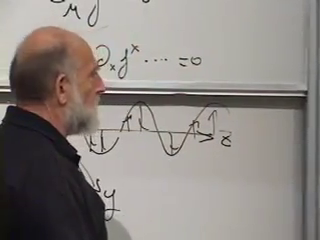
\includegraphics[width=0.70\textwidth]{lecture_58_figure_05.png}
\caption{완성된 횡전자기파 판서 그림. 전기장과 자기장의 진동 방향은 서로 수직이며 전파 방향에도 수직이다.}
\lectureframe{01:05:25}
\end{figure}

\begin{figure}[H]
\centering
\scalebox{0.90}{%
\begin{tikzpicture}[x=1cm,y=1cm,>=Latex]
  \draw[->,thick] (0,0) -- (8.2,0) node[right] {$z$};
  \draw[->,thick] (0,-1.6) -- (0,1.7) node[above] {$x$};
  \draw[->,thick] (0,0) -- (-1.15,-0.8) node[below left] {$y$};
  \draw[blue!70!black,thick,domain=0:7.5,samples=120]
    plot (\x,{0.95*sin(90*\x)});
  \foreach \z/\s in {0.8/1,2.8/-1,4.8/1,6.8/-1}{
    \draw[->,green!45!black,thick]
      (\z,0) -- ++({-0.55*\s},{-0.38*\s});
  }
  \node[blue!70!black] at (6.9,1.25) {$\mathbf E$};
  \node[green!45!black] at (5.2,-1.05) {$\mathbf B$};
  \draw[->,very thick] (6.2,1.55) -- (7.7,1.55)
    node[midway,above] {propagation};
\end{tikzpicture}
}
\caption{\(\mathbf E\)와 \(\mathbf B\)는 서로 수직이고,
전파 방향에도 수직입니다.}
\end{figure}

이것이 빛과 진공 속 모든 전자기 복사의 특성입니다. 파동을 만들어 낸 방정식이 로런츠 공변이므로, 다른 관성계의 관찰자도 횡방향 전기장과 자기장을 가진 전자기파가 \(c\)의 속도로 움직인다고 기술합니다.

\section{전하 밀도와 전류 밀도}

이제 잠시 미뤄 두었던 원천을 다시 포함하겠습니다. 한 영역에 하전 입자가 많이 있을 때는 이들을 연속적인 전하 밀도로 거시적으로 묘사하는 것이 편리합니다.
\begin{equation}
\rho(\mathbf x,t)=\frac{dQ}{dV}.
\end{equation}
분자로 이루어진 물을 연속적인 유체로 취급하는 것과 비슷한 근사입니다. 양전하와 음전하는 서로 반대 부호로 기여하므로, \(\rho\)는 단위 부피당 알짜 전하입니다.

정해진 영역 \(V\) 안의 전하는 다음과 같습니다.
\begin{equation}
Q_V(t)=\int_V\rho(\mathbf x,t)\,dV.
\label{eq:charge-volume}
\end{equation}
밀도는 위치와 시간에 따라 변할 수 있습니다. 한곳에 모여 있던 전하가 빠져나가면 그곳의 국소 밀도는 변합니다. 그러나 밀도가 임의의 방식으로 변할 수는 없습니다. 자연에서는 전하가 보존됩니다.

전역적인 보존만으로는 조건이 너무 약합니다. 전체 전하가 그대로인 채 지구에서 전하가 사라졌다가 같은 순간 화성에서 다시 나타나는 것도 허용하게 되기 때문입니다. 더 강한 조건은 국소적입니다. 전하는 그 사이 공간을 흐르지 않고서는 한곳을 떠나 다른 곳에 도달할 수 없습니다.

그 흐름을 기술하기 위해 방향을 정한 미소 면적 요소
\begin{equation}
d\boldsymbol\sigma=\widehat{\mathbf n}\,d\sigma.
\end{equation}
를 생각합시다. 크기는 면적이고 방향은 면에 수직입니다. 전류 밀도 \(\mathbf J\)는 이 요소를 단위 시간에 통과하는 전하가 다음과 같도록 정의합니다.
\begin{equation}
\frac{dQ}{dt}=\mathbf J\cdot d\boldsymbol\sigma.
\label{eq:current-flux-element}
\end{equation}
\(\mathbf J\)의 크기는 단위 면적·단위 시간당 전하량이며, 방향은 양전하가 흐르는 방향입니다.

\begin{figure}[H]
\centering
\includegraphics[width=0.64\textwidth]{lecture_58_figure_10.png}
\caption{방향이 정해진 면적 요소와 플럭스 인자 \(d\boldsymbol\sigma\cdot\mathbf J\).}
\lectureframe{01:18:15}
\end{figure}

내적은 면에 수직인 성분만 골라냅니다. 면에 접하는 전류는 어느 쪽으로도 면을 통과하지 않으므로 기여가 0입니다. 면의 법선과 나란한 전류는 크기가 일정할 때 플럭스가 최대입니다. 도선의 전류는 한 가지 특수한 경우일 뿐이며, \(\mathbf J\)는 판을 통과하거나 3차원 공간 전체를 흐르는 전하도 기술할 수 있습니다.

\section{국소 보존과 연속 방정식}

공간에서 영역 \(V\)를 고정하고, 그 닫힌 경계 \(\partial V\)의 모든 요소가 바깥쪽을 향하도록 방향을 정합시다. 순유출 전류가 있으면 내부 전하는 감소합니다.
\begin{equation}
\frac{dQ_V}{dt}
=-\oint_{\partial V}\mathbf J\cdot d\boldsymbol\sigma.
\label{eq:integral-conservation}
\end{equation}
마이너스 부호는 단순한 규약이 아니라 물리적 의미를 가집니다. 바깥쪽으로 나가는 양의 플럭스는 영역 안의 양전하를 줄입니다. 방정식~\eqref{eq:charge-volume}을 사용하면,
\begin{equation}
\int_V\partial_t\rho\,dV
=-\oint_{\partial V}\mathbf J\cdot d\boldsymbol\sigma.
\label{eq:integral-continuity-one}
\end{equation}

\begin{figure}[H]
\centering
\includegraphics[width=0.72\textwidth]{lecture_58_figure_11.png}
\caption{면 플럭스를 부피에 관한 식으로 바꾼 뒤 얻은 고정 영역의 보존 법칙.}
\lectureframe{01:29:00}
\end{figure}

발산 정리라고도 부르는 가우스 정리는 닫힌 면을 통과하는 플럭스를 내부의 발산과 연결합니다.
\begin{equation}
\oint_{\partial V}\mathbf A\cdot d\boldsymbol\sigma
=\int_V\boldsymbol\nabla\cdot\mathbf A\,dV.
\label{eq:divergence-theorem}
\end{equation}
그릇 안의 여러 지점에서 물을 주입하는 숨은 관을 떠올려 볼 수 있습니다. 발산은 관 끝에서 물이 나오는 국소적인 비율을 나타내고, 면적분은 그릇 밖으로 나가는 물의 총량을 나타냅니다. 내부에서 바깥쪽 흐름으로 생성된 물은 결국 경계를 통과해야 합니다.

식~\eqref{eq:divergence-theorem}을 \(\mathbf J\)에 적용하면
\begin{equation}
\int_V
\left(\partial_t\rho+\boldsymbol\nabla\cdot\mathbf J\right)dV=0.
\end{equation}
이 관계는 가능한 모든 영역 \(V\)에 대해 성립한다. 따라서 피적분함수는 각 점에서 영이어야 한다.
\begin{equation}
\boxed{\partial_t\rho+\boldsymbol\nabla\cdot\mathbf J=0.}
\label{eq:continuity-three}
\end{equation}

\begin{figure}[H]
\centering
\includegraphics[width=0.72\textwidth]{lecture_58_figure_12.png}
\caption{성분별로 쓴 국소 연속 방정식.}
\lectureframe{01:29:50}
\end{figure}

방정식~\eqref{eq:continuity-three}은 국소 보존이 요구하는 내용을 정확히 말해 줍니다. 한 점 또는 작은 영역에서 전하 밀도가 감소한다면 전류가 그곳에서 바깥으로 발산해야 합니다. 전류가 안쪽으로 모이면 전하 밀도는 증가합니다.

밀도와 전류는 자연스럽게 4-전류를 이룹니다.
\begin{equation}
J^\mu=(\rho,J_x,J_y,J_z)
\label{eq:four-current}
\end{equation}
\(c=1\) 단위계에서 연속 방정식은 로런츠 스칼라 방정식이 됩니다.
\begin{equation}
\partial_\mu J^\mu=0.
\label{eq:continuity-four}
\end{equation}
상대론적 분포의 흐름은 한 입자의 4-속도와 마찬가지로 4-벡터처럼 변환해야 합니다. 방정식~\eqref{eq:continuity-four}은 모든 관성계에서 국소 전하 보존이 성립하게 합니다.

\section{원천이 있는 맥스웰 방정식}

전하와 전류를 다시 포함하면 다음과 같습니다.
\begin{align}
\boldsymbol\nabla\cdot\mathbf E&=\rho,
\label{eq:gauss-e-source}\\
\boldsymbol\nabla\cdot\mathbf B&=0,\\
\boldsymbol\nabla\times\mathbf E&=-\partial_t\mathbf B,\\
\boldsymbol\nabla\times\mathbf B&=\partial_t\mathbf E+\mathbf J.
\label{eq:ampere-source}
\end{align}
전기 원천이 들어가는 방정식들은 다음 식으로 간결해집니다.
\begin{equation}
\boxed{\partial_\mu F^{\mu\nu}=J^\nu,}
\label{eq:maxwell-source-covariant}
\end{equation}
자기장에 대한 원천 없는 두 방정식은 그대로입니다.
\begin{equation}
\boxed{\partial_\mu\widetilde F^{\mu\nu}=0.}
\label{eq:maxwell-dual-source}
\end{equation}

\begin{figure}[H]
\centering
\includegraphics[width=0.78\textwidth]{lecture_58_figure_13.png}
\caption{원천이 있는 맥스웰 방정식과 그 공변 형태 \(\partial_\mu F^{\mu\nu}=J^\nu\).}
\lectureframe{01:34:00}
\end{figure}

방정식~\eqref{eq:maxwell-source-covariant}의 시간 성분은 다음과 같습니다.
\begin{equation}
\partial_\mu F^{\mu t}=J^t=\rho,
\end{equation}
앞서 수행한 성분 계산에 따르면 좌변은 \(\boldsymbol\nabla\cdot\mathbf E\)가 됩니다. 세 공간 성분은 다음을 재현합니다.
\(\boldsymbol\nabla\times\mathbf B=\partial_t\mathbf E+\mathbf J\)

유용한 일관성 검산도 가능합니다. \(\partial_\nu\)를 방정식~\eqref{eq:maxwell-source-covariant}에 적용하면 다음을 얻습니다.
\begin{equation}
\partial_\nu J^\nu
=\partial_\nu\partial_\mu F^{\mu\nu}=0,
\end{equation}
두 미분은 \(\mu\leftrightarrow\nu\)에 대해 대칭인 반면 \(F^{\mu\nu}\)는 반대칭이기 때문입니다.\editorialnote{이 짧은 일관성 검산은 공변 방정식에서 바로 따라 나오며, 원천이 있는 맥스웰 방정식이 연속 방정식을 자동으로 만족하는 이유를 명시적으로 보여 줍니다.}

이제 상호적인 구조가 완성되었습니다. 텐서 힘 법칙
\(f^\mu=qF^\mu{}_\nu u^\nu\)은 장이 전하에 어떻게 작용하는지 기술하고, 방정식~\eqref{eq:maxwell-source-covariant}은 전하와 전류가 장을 어떻게 만들어 내는지 기술합니다. 둘 다 텐서 방정식입니다. 진공에서는 같은 장 방정식이 \(c\)의 속도로 움직이는 횡파를 낳습니다. 이처럼 로런츠 공변성과 전자기파 방정식은 이 구성을 이끈 출발점에서 만납니다. 모든 관성계의 관찰자는 같은 전자기 법칙과 같은 빛의 속도를 얻습니다.

\chapter{고유 시간, 시간 지연, 길이 수축}

우리는 흔히 빛의 속도를 $c=1$로 두는 단위계를 택한다. 이 단위계에서는 한 해라는 시간과 한 광년이라는 거리를 직접 비교할 수 있어 식을 훨씬 읽기 쉽다. $c$이 물리적으로 중요할 때는 그 값을 다시 명시하겠다. 차원 분석만으로도 그 값이 어디에 들어가는지 알 수 있다.

\section{갈릴레이 시공간 격자}

정지한 기준계와 $x$축을 따라 속도 $v$로 움직이는 기차 사이의 아인슈타인 이전 관계부터 살펴봅시다.
\begin{align}
x' &= x-vt, & t'&=t.
\label{eq:l4-galilean}
\end{align}
두 번째 식에는 뉴턴의 보편적 시간 가정이 담겨 있습니다. 공간의 원점은 서로에 대해 움직이지만, 모든 관측자는 같은 동시성 단면을 사용합니다.

프라임이 없는 좌표계의 관측자는 선로 옆에 서 있고, 프라임 좌표계의 관측자는 기차에 타 있다고 합시다. 기차의 원점은 $x'=0$이므로, 프라임이 없는 좌표계에서 그 세계선은 다음과 같습니다.
\begin{equation}
x=vt.
\end{equation}
이 기울어진 선이 $t'$축입니다. 반면 $t'=t$는 모든 $t'$ 일정선이 $t$ 일정선과 같은 수평선임을 뜻합니다.

\begin{figure}[H]
\centering
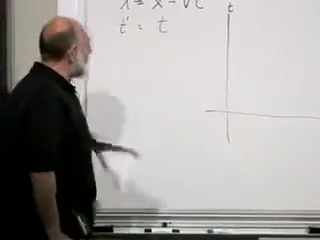
\includegraphics[width=0.72\textwidth]{lecture_04_figure_02.png}
\caption{$t$-$x$ 초기 격자와 갈릴레이 변환. 움직이는 원점은 $x=vt$을 따라가며, 두 기준계는 동일한 일정 시간선을 유지합니다.}
\lectureframe{00:03:06}
\end{figure}

식~\eqref{eq:l4-galilean}에서 프라임이 없는 좌표를 구하면 다음과 같습니다.
\begin{align}
x&=x'+vt'=x'+vt, & t&=t'.
\end{align}
역변환은 $v$을 $-v$로 바꾸면 같은 형태가 됩니다. 기차가 역에 대해 앞으로 움직이면 역은 기차에 대해 뒤로 움직입니다. 이 상호성은 특수 상대성 이론에서도 유지되지만, 보편적 시간은 그렇지 않습니다.

\section{로런츠 보정}

갈릴레이 변환으로는 모든 관성계에서 빛의 속도가 같게 되지 않습니다. 보정된 관계식은 먼저 $c=1$ 단위로 쓰면 다음과 같습니다.
\begin{align}
x'&=\frac{x-vt}{\sqrt{1-v^2}}, &
t'&=\frac{t-vx}{\sqrt{1-v^2}}.
\label{eq:l4-lorentz-natural}
\end{align}
일반적인 단위로 되돌리면 다음과 같습니다.
\begin{align}
x'&=\frac{x-vt}{\sqrt{1-v^2/c^2}}, &
t'&=\frac{t-vx/c^2}{\sqrt{1-v^2/c^2}}.
\label{eq:l4-lorentz-c}
\end{align}

\begin{figure}[H]
\centering
\includegraphics[width=0.74\textwidth]{lecture_04_figure_05.png}
\caption{인자 $c$를 다시 넣은 로런츠 변환.}
\lectureframe{00:09:10}
\end{figure}

$v\ll c$일 때, 뉴턴 역학이 적용되는 상황에서는 $v^2/c^2$과 $vx/c^2$가 모두 매우 작습니다. 그러면 식~\eqref{eq:l4-lorentz-c}은 갈릴레이 결과로 환원됩니다. 상대성 이론은 뉴턴 운동학을 폐기하지 않고, 그 유효 범위를 밝혀 줍니다.

$v=c$에서는 분모가 영이 된다. 관성계는 다른 관성계에 대해 빛의 속도로 움직일 수 없다. 그 한계에서 충분히 멀리 떨어져 있으면 보정은 작지만, 한계에 가까워지면 $x$와 $t$의 혼합을 피할 수 없다.

운동 방향을 $x$로 정했으므로, 횡방향 좌표는 변하지 않습니다.
\begin{equation}
y'=y,\qquad z'=z.
\end{equation}
그 이유를 살펴보는 한 가지 방법은 기차와 승강장에 똑같은 횡방향 미터자를 놓는 것입니다. 두 기준계의 중간에서 움직이는 관측자는 막대들이 서로 반대 방향으로 같은 속도로 다가오는 것을 봅니다. 이 설정에는 어느 한쪽 횡방향 막대를 다른 쪽보다 짧게 만들 만한 특징이 없습니다.

\section{빛원뿔을 따른 로런츠 변환}

식~\eqref{eq:l4-lorentz-natural}을 기하학적으로 읽는 방법이 있습니다. 두 식을 더하면 다음과 같습니다.
\begin{align}
t'+x'
&=\frac{(t-vx)+(x-vt)}{\sqrt{1-v^2}}\\
&=(t+x)\frac{1-v}{\sqrt{1-v^2}}\\
&=(t+x)\sqrt{\frac{1-v}{1+v}}.
\label{eq:l4-null-plus}
\end{align}
이번에는 순서를 바꾸어 빼면 다음과 같습니다.
\begin{align}
t'-x'
&=\frac{(t-vx)-(x-vt)}{\sqrt{1-v^2}}\\
&=(t-x)\frac{1+v}{\sqrt{1-v^2}}\\
&=(t-x)\sqrt{\frac{1+v}{1-v}}.
\label{eq:l4-null-minus}
\end{align}

\begin{figure}[H]
\centering
\includegraphics[width=0.75\textwidth]{lecture_04_figure_06.png}
\caption{영벡터 조합 $t+x$과 $t-x$로 다시 쓴 로런츠 변환. 두 조합의 스케일 인자는 서로 역수입니다.}
\lectureframe{00:18:45}
\end{figure}

조합 $t+x$과 $t-x$은 두 $45^\circ$ 광선 방향을 따른 좌표입니다. 부스트는 이 방향 중 하나를 수축시키고 다른 하나를 역수 인자만큼 늘립니다. 어느 방향도 $45^\circ$에서 벗어나 회전하지 않습니다. 따라서 빛선은 계속 빛선으로 남으며, 이것이 빛의 불변 속도를 보여 주는 시공간 그림입니다.

\begin{classroomqa}\audiencequestion{중간 기준계의 관측자가 대칭적인 실험을 본다고 해서, 기차와 승강장 관측자에게도 같은 결과가 성립한다는 점을 어떻게 알 수 있나요?\lecturetimestamp{00:20:48}}\lecturerresponse{여기에는 한 가지 사실이 더 쓰입니다. 사건의 일치는 불변입니다. 막대의 양 끝이 만나면, 그 만남은 하나의 시공간 사건입니다. 모든 관성 관측자는 그 사건에 서로 다른 좌표를 부여할 수 있지만, 하나의 일치를 서로 다른 두 위치로 나눌 수는 없습니다. 서로 대응하는 끝점이 만나는 곳에서 섬광을 내보내면 그 사건을 실험적으로 검출할 수 있습니다. 중간 기준계의 대칭성과 두 끝점 만남의 불변성으로 횡방향 길이가 같음을 알 수 있습니다.}\end{classroomqa}

\begin{classroomqa}\audiencequestion{중간 기준계를 나타내는 자전거 타는 사람은 실제로 막대의 중간 지점에 있어야 하나요?\lecturetimestamp{00:22:25}}\lecturerresponse{아닙니다. 기준계란 한곳에 있는 한 사람의 눈이 아니라, 관측자와 시계로 이루어진 전체 네트워크입니다. 자전거 타는 사람은 끝점에서 나온 섬광을 나중에 받아 그 섬광이 어디서 나왔는지 추론할 수 있습니다. 중요한 것은 빛을 나중에 받은 위치가 아니라 각 방출 사건의 시공간상 위치입니다.}\end{classroomqa}

연속된 속도를 합성하는 일도 같은 변환에서 나오는 결과지만, 다음 강의로 미루겠습니다. 이번에는 움직이는 시계가 측정하는 불변량을 확인하는 것이 목표입니다.

\section{불변 간격}

일반적인 데카르트 좌표축을 회전하면 양 $x^2+y^2$는 변하지 않습니다. 로런츠 변환은 다른 이차 형식을 보존합니다. 식~\eqref{eq:l4-lorentz-natural}에서
\begin{align}
t'^2-x'^2
&=\frac{(t-vx)^2-(x-vt)^2}{1-v^2}\\
&=\frac{t^2-2vtx+v^2x^2-x^2+2vtx-v^2t^2}{1-v^2}\\
&=t^2-x^2.
\label{eq:l4-interval}
\end{align}
교차항은 상쇄되고, 남은 분자에는 $1-v^2$이라는 공통 인자가 들어 있습니다.

\begin{figure}[H]
\centering
\includegraphics[width=0.76\textwidth]{lecture_04_figure_07.png}
\caption{$t'^2-x'^2=t^2-x^2$의 판서 유도.}
\lectureframe{00:33:15}
\end{figure}

공간 차원이 세 개일 때 불변량은 다음과 같습니다.
\begin{equation}
t'^2-x'^2-y'^2-z'^2=t^2-x^2-y^2-z^2
\end{equation}
$c=1$ 단위에서 그렇습니다. 더 일반적으로 두 사건 사이에는 좌표 차이를 사용합니다.
\begin{equation}
\Delta s^2
=c^2\Delta t^2-\Delta x^2-\Delta y^2-\Delta z^2.
\label{eq:l4-spacetime-interval}
\end{equation}
각 관성 관측자는 시간 항과 공간 항의 값에는 동의하지 않더라도 이 수치에는 동의합니다.

\section{고유 시간과 움직이는 시계}

빛 신호를 주고받아 시계를 동기화한 정지 관측자들의 격자를 생각해 봅시다. 이들의 시계가 가리키는 값으로 좌표 시간 $t$를 정합니다. 이제 손목시계 하나를 그 격자 안에서 움직여 봅시다. 손목시계 자체의 표시는 그 세계선을 따라가며, 그 표시가 고유 시간입니다.

시간꼴로 분리된 두 사건에 대해 다음과 같이 정의합니다.
\begin{equation}
c^2\Delta\tau^2
=c^2\Delta t^2-\Delta x^2-\Delta y^2-\Delta z^2.
\label{eq:l4-proper-time}
\end{equation}
$c=1$인 한 공간 차원에서는 단순히 다음과 같습니다.
\begin{equation}
\Delta\tau=\sqrt{\Delta t^2-\Delta x^2}.
\end{equation}
제곱근은 보통 거리의 공식과 비슷하지만, 마이너스 부호 때문에 기하학이 달라집니다.

경우는 세 가지입니다.
\begin{align}
\Delta t^2-\Delta x^2 &>0 &&\text{timelike},\\
\Delta t^2-\Delta x^2 &=0 &&\text{lightlike},\\
\Delta t^2-\Delta x^2 &<0 &&\text{spacelike}.
\end{align}
빛원뿔 안쪽에서는 고유 시간이 실수입니다. 원뿔 위에서는 $x=\pm t$이므로 사건들이 일치하지 않아도 고유 시간은 0입니다. 빛선은 바로 이런 사건들을 연결할 수 있습니다. 원뿔 바깥쪽에서는 분리가 공간꼴입니다. 이때는 시계 시간의 허수값보다 실수인 고유 거리 $\sqrt{\Delta x^2-\Delta t^2}$로 나타내는 편이 적절합니다.

\begin{figure}[H]
\centering
\includegraphics[width=0.73\textwidth]{lecture_04_figure_08.png}

\vspace{0.8em}

\begin{tikzpicture}[x=1.0cm,y=1.0cm]
\draw[->] (-3.3,0) -- (3.3,0) node[right] {$x$};
\draw[->] (0,-0.4) -- (0,4.0) node[above] {$t$};
\draw[thick] (0,0) -- (3.0,3.0) node[above right] {$x=t$};
\draw[thick] (0,0) -- (-3.0,3.0) node[above left] {$x=-t$};
\node at (0,2.0) {timelike};
\node at (2.25,1.05) {spacelike};
\node at (-2.25,1.05) {spacelike};
\end{tikzpicture}\caption{시간꼴, 빛꼴, 공간꼴 분리를 명확하게 구분한 판서 빛원뿔.}\lectureframe{00:38:40}
\end{figure}

식~\eqref{eq:l4-proper-time}은 왜 시계의 표시와 같을까요? 정지한 시계에서는 $\Delta x=0$이므로 $\Delta\tau=\Delta t$입니다. 등속 운동하는 시계의 경우, 그 시계가 정지해 있는 프라임 좌표계를 택합시다. 그 좌표계에서는 $\Delta x'=0$이고, 불변성에 따라
\begin{equation}
\Delta\tau
=\sqrt{\Delta t'^2-\Delta x'^2}
=\Delta t'.
\end{equation}
따라서 움직이는 시계가 기록하는 것은 고유 시간입니다.

\begin{classroomqa}\audiencequestion{``사건 사이의 간격''과 ``시계가 가리키는 값''은 같은 것을 가리키는 두 가지 이름인가요?\lecturetimestamp{00:44:49}}\lecturerresponse{이상적인 시계가 한 사건에서 다른 사건까지 관성 운동을 하면 두 값은 일치합니다. 불변 간격은 기하학적 양이고, 함께 움직이는 시계의 두 끝점 표시 차이는 그 양을 물리적으로 측정한 값입니다. 정지한 좌표계의 시계는 일반적으로 이와 다른 좌표 시간 간격을 기록합니다.}\end{classroomqa}

\section{시간 지연과 동시성}

움직이는 좌표계의 원점을 생각해 봅시다. 그 세계선은 다음 관계를 따릅니다.
\begin{equation}
x'=0,\qquad x=vt.
\end{equation}
기울어진 이 선은 움직이는 시계의 경로이자 $t'$축입니다.

\begin{figure}[H]
\centering
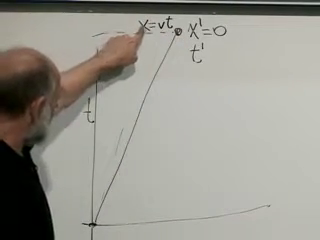
\includegraphics[width=0.72\textwidth]{lecture_04_figure_03.png}
\caption{움직이는 원점: $x=vt$, $x'=0$, $t'$축은 모두 같은 세계선을 가리키는 세 가지 표현입니다.}
\lectureframe{00:48:18}
\end{figure}

공통 원점과 그 세계선 위의 나중 점 사이에 불변 간격을 적용하면 다음과 같습니다.
\begin{align}
t'^2-x'^2&=t^2-x^2,\\
t'^2&=t^2-v^2t^2,\\
t'&=t\sqrt{1-v^2}.
\label{eq:l4-time-dilation-natural}
\end{align}
$c$를 다시 표시하면
\begin{equation}
\Delta\tau=\Delta t\sqrt{1-\frac{v^2}{c^2}}
=\frac{\Delta t}{\gamma},
\qquad
\gamma=\frac{1}{\sqrt{1-v^2/c^2}}.
\label{eq:l4-time-dilation}
\end{equation}

\begin{figure}[H]
\centering
\includegraphics[width=0.73\textwidth]{lecture_04_figure_09.png}
\caption{판서에 나온 시간 지연 결과: $c=1$ 단위에서 움직이는 시계가 누적하는 시간은 $t'=t\sqrt{1-v^2}$입니다.}
\lectureframe{00:50:45}
\end{figure}

정지 관측자는 움직이는 시계가 느리게 간다고 말합니다. 상호성에 따라 움직이는 관측자도 정지한 시계가 느리게 간다고 말해야 합니다. 두 설명은 서로 다른 원거리 사건 쌍을 비교하므로 모순이 아닙니다.

실제로 식~\eqref{eq:l4-lorentz-natural}에서 $t'$가 일정한 값이면 다음 관계를 만족합니다.
\begin{equation}
t-vx=\text{constant}.
\label{eq:l4-simultaneity}
\end{equation}
움직이는 관측자의 동시성 선은 수평선 $t=\text{constant}$에 대해 기울어져 있습니다. 관측자마다 서로 다른 원거리 시계 표시들을 동시에 일어난 것으로 봅니다. 이 차이를 분명히 해 두면 시계가 서로에게 상대적으로 느리게 간다는 결과는 모순 없이 양립합니다.

\begin{figure}[H]
\centering
\begin{tikzpicture}[x=1cm,y=1cm]
\draw[->] (0,0) -- (0,4.2) node[above] {$t$};
\draw[->] (0,0) -- (5.2,0) node[right] {$x$};
\draw[thick,->] (0,0) -- (2.4,3.8) node[above] {$x'=0$};
\draw[dashed] (0,2.8) -- (4.8,2.8)
  node[right] {$t=\mathrm{const}$};
\draw[thick] (0.15,1.05) -- (4.7,2.35)
  node[right] {$t'=\mathrm{const}$};
\draw[thick] (3.4,0) -- (3.4,3.8);
\fill (3.4,2.8) circle (0.045);
\fill (3.4,1.98) circle (0.045);
\end{tikzpicture}
\caption{상호적 시간 지연은 서로 다른 동시성 단면 위의 시계 표시를 비교합니다.}
\end{figure}

\section{쌍둥이의 경로}

두 쌍둥이는 같은 사건에서 출발합니다. 한 명은 $x=0$에 머뭅니다. 다른 한 명은 속도 $v$로 바깥쪽으로 이동했다가 방향을 바꾸어 같은 속도로 돌아옵니다. 다시 만났을 때 손목시계, 심장 박동, 신진대사, 노화 자체처럼 시계 역할을 할 수 있는 모든 물리적 과정의 결과를 비교합니다.

집에 남은 쌍둥이의 기준계에서 여정의 각 절반이 좌표 시간 $T$만큼 걸린다고 합시다. 집에 남은 쌍둥이의 고유 시간은 다음과 같습니다.
\begin{equation}
\tau_{\mathrm{home}}=2T.
\end{equation}
방향을 바꾸는 사건의 좌표는 $(vT,T)$입니다. 따라서 여행의 첫 구간에서 누적되는 고유 시간은
\begin{align}
\tau_{\mathrm{leg}}
&=\sqrt{T^2-v^2T^2}
=T\sqrt{1-v^2}.
\end{align}
돌아오는 구간에서도 같은 만큼 누적되므로
\begin{equation}
\tau_{\mathrm{travel}}=2T\sqrt{1-v^2}<2T.
\label{eq:l4-twin}
\end{equation}

\begin{figure}[H]
\centering
\includegraphics[width=0.73\textwidth]{lecture_04_figure_10.png}

\vspace{0.8em}

\begin{tikzpicture}[x=1.1cm,y=1cm]
\draw[->] (-0.2,0) -- (3.4,0) node[right] {$x$};
\draw[->] (0,-0.1) -- (0,4.4) node[above] {$t$};
\draw[very thick] (0,0) -- (0,4);
\draw[very thick] (0,0) -- (2.2,2) -- (0,4);
\draw[dashed] (0,2) -- (2.2,2);
\node[left] at (0,2) {$T$};
\node[left] at (0,4) {$2T$};
\node[below right] at (1.1,1.0) {$v$};
\node[above right] at (1.1,3.0) {$-v$};
\end{tikzpicture}\caption{집에 남은 쌍둥이의 세계선과 여행자의 두 구간. 시공간을 지나는 경로가 서로 다르므로 이들의 고유 시간도 다릅니다.}\lectureframe{00:59:35}
\end{figure}

나이가 서로 달라도 모순은 없습니다. 여행자의 경로에는 방향 전환이 있고, 하나의 관성계 대칭 변환으로 집에 남은 쌍둥이의 직선 경로와 연결되지 않습니다. 보통의 유클리드 기하에서도 두 점을 잇는 직선 경로와 꺾인 경로의 길이는 다릅니다. 민코프스키 기하에서는 어느 경로의 간격이 더 큰지가 반대가 되지만, 비교 자체는 여전히 기하학적입니다.

\section{가속과 이상적인 시계}

\begin{classroomqa}\audiencequestion{방향을 바꾸는 순간에는 물리가 달라지고 여행자가 가속합니다. 그러면 시계 계산이 무효가 되나요?\lecturetimestamp{01:02:19}}\lecturerresponse{가속은 실제로 존재하며 비대칭을 드러내는 데 도움이 됩니다. 가속을 없던 일처럼 취급해서는 안 됩니다. 날카로운 모서리는 이상화한 그림일 뿐이므로 유한한 시간 동안 부드럽게 방향을 바꾸도록 그릴 수 있습니다. 여기에는 추가적인 물리적 가정도 필요합니다. 충분히 작고 잘 만들어진 시계는 적당한 가속에 민감하지 않아 계속 고유 시간을 기록한다는 가정입니다. 크거나 깨지기 쉬운 시계는 변형되거나 망가질 수 있지만, 그것은 시공간 간격의 문제가 아니라 시계 장치의 결함입니다.}\end{classroomqa}

이 이상적인 시계에 관한 가정은 로런츠 변환만으로 유도되지 않습니다. 실제 시계 장치의 거동을 통해 검증해야 합니다. 원자는 수백 마일 크기의 시계보다 훨씬 좋은 근사물입니다. 작은 장치는 가속이나 중력으로 변형되기 어렵기 때문입니다. 일반 상대성 이론을 언급한다고 해서 이 물리적 문제가 사라지는 것은 아닙니다. 선택한 장치가 주변 환경에 어떻게 반응하는지 여전히 알아야 합니다.

\begin{classroomqa}\audiencequestion{가속하는 궤적을 짧은 구간들로 나누어 각 구간에서 관성계 분석을 적용할 수 있나요?\lecturetimestamp{01:09:08}}\lecturerresponse{가능합니다. 곡선을 짧고 거의 직선인 구간들로 나누어 각 구간의 고유 시간을 계산한 다음, 결과를 더하면 됩니다. 이는 많은 짧은 선분으로 보통 곡선의 길이를 구하는 것과 비슷한 시공간상의 방법입니다. 연속체 극한에서는
\[
\tau=\int \sqrt{1-\frac{v(t)^2}{c^2}}\,dt,
\]
관성 좌표계로 기술하는 평탄한 시공간에서의 운동에 대해 이 식이 성립합니다.}\end{classroomqa}

\section{쌍둥이가 보는 것}

빛 펄스를 보내면 최종 시계 표시를 실험적으로 확인할 수 있습니다. 두 세계선에서 고유 시간 1초 간격을 표시하고, 쌍둥이 각자가 표시가 있을 때마다 펄스를 내보내게 합시다. 바깥쪽으로 가는 동안에는 상대방에게서 받은 펄스 사이 간격이 벌어집니다. 돌아오는 동안에는 펄스가 뭉쳐서 도착합니다. 이는 시공간 그림에 직접 나타낸 상대론적 도플러 효과입니다.

\begin{figure}[H]
\centering
\includegraphics[width=0.73\textwidth]{lecture_04_figure_11.png}
\caption{집에 남은 쌍둥이와 여행자의 세계선 사이에서 주고받는 빛 신호. 바깥쪽으로 가는 구간에서는 펄스가 드문드문 도착하고, 돌아오는 구간에서는 도착 간격이 줄어듭니다. 이로써 방출된 모든 펄스를 빠짐없이 설명할 수 있습니다.}
\lectureframe{01:12:55}
\end{figure}

이 이야기의 어떤 시간 구간도 사라지지 않습니다. 각 관측자는 결국 상대방이 보낸 모든 펄스를 받지만, 수신율은 상대 운동에 따라 달라집니다. 두 경로에서 적색편이와 청색편이가 지속되는 시간은 같지 않으므로, 받은 펄스를 모두 세면 고유 시간 비교와 일치합니다.

\begin{classroomqa}\audiencequestion{돌아오는 여행자가 청색편이된 빛을 받는다면, 방출원이 낸 에너지보다 더 많은 에너지를 얻을 수 있나요?\lecturetimestamp{01:13:50}}\lecturerresponse{이 질문에 답하려면 아직 다루지 않은 에너지의 상대론적 정의와 기준계 의존성을 알아야 합니다. 타당한 질문이지만, 특히 가속 관측자의 경우 좌표와 펄스 수만으로는 에너지 수지를 따질 수 없습니다. 그러므로 답을 추측하기보다 뒤로 미루어야 합니다.}\end{classroomqa}

\section{닫힌 공간 방향}

\begin{classroomqa}\audiencequestion{공간 방향 하나가 콤팩트하다고 합시다. 쌍둥이 한 명이 그 방향을 따라 등속 운동하여 출발점으로 돌아오면서 가속을 완전히 피할 수 있을까요? 그렇다면 두 쌍둥이를 구별하는 것은 무엇인가요?\lecturetimestamp{01:15:14}}\lecturerresponse{공간은 더 큰 공간 안에 구부러진 면이 아니라, 그 자체로 원통인 공간으로 상상해야 합니다. 방사 방향 가속은 없어도 됩니다. 그래도 돌아온 관측자는 같은 장소가 되풀이된다는 전역적 사실을 마주하게 됩니다. 이는 비대칭이 있음을 보여 주지만, 완전한 답을 위해서는 공간을 동일시하는 특수 상대성 이론을 신중하게 다루어야 합니다. 여기서는 즉흥적으로 답하지 않고 열린 질문으로 남겨 둡니다.}\end{classroomqa}

\begin{figure}[H]
\centering
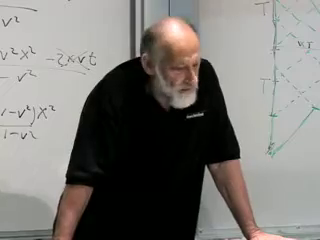
\includegraphics[width=0.72\textwidth]{lecture_04_figure_04.png}

\vspace{0.8em}

\begin{tikzpicture}[x=1cm,y=1cm]
\draw[thick] (0,0) ellipse (1.3 and 0.35);
\draw[thick] (-1.3,0) -- (-1.3,-3.1);
\draw[thick] (1.3,0) -- (1.3,-3.1);
\draw[thick] (0,-3.1) ellipse (1.3 and 0.35);
\draw[->,very thick] (0.0,0.38) arc (90:-210:1.38 and 0.42);
\node[right] at (1.65,-1.5) {compact spatial direction};
\end{tikzpicture}\caption{판서에 그린 콤팩트 공간 질문과 깔끔한 내재적 원통. 이 질문은 추가적인 방사 차원에 놓인 원통 주위의 운동이 아니라 전역적 동일시에 관한 것입니다.}\lectureframe{01:17:56}
\end{figure}

\section{동시성 단면에서 측정하는 길이}

특수 상대성 이론 문제에서는 먼저 시공간 그림을 그립니다. 프라임이 없는 기준계에서 정지해 있는 미터자를 생각해 봅시다. 양 끝점은 $x=0$과 $x=1$에 있습니다. 시간이 흐르면 두 끝점은 수직 세계선을 그립니다. 막대는 그 사이의 시공간 영역을 쓸어 냅니다.

움직이는 관측자는 움직이는 시간 $t'$가 한 값일 때 두 끝점을 모두 측정해야 합니다. 식~\eqref{eq:l4-simultaneity}에서 원점을 지나며 $t'=0$인 단면은 다음 관계를 만족합니다.
\begin{equation}
t=vx
\end{equation}
$c=1$ 단위에서 그렇습니다. 이 단면은 $x=1$인 오른쪽 끝점과 $t=v$에서 만납니다.

\begin{figure}[H]
\centering
\includegraphics[width=0.73\textwidth]{lecture_04_figure_12.png}

\vspace{0.8em}

\begin{tikzpicture}[x=1.55cm,y=1.15cm]
\draw[->] (-0.5,0) -- (3.1,0) node[right] {$x$};
\draw[->] (0,0) -- (0,3.8) node[above] {$t$};
\draw[very thick,red] (0,0) -- (0,3.3);
\draw[very thick,red] (2.15,0) -- (2.15,3.3);
\fill[red!12] (0,0) rectangle (2.15,3.3);
\draw[very thick,green!50!black] (0,0) -- (1.2,3.1)
  node[above] {$x=vt$};
\draw[very thick,blue] (0,0) -- (2.15,1.15)
  node[right] {$t'=0$};
\fill (2.15,1.15) circle (0.045);
\node[right] at (2.22,1.35) {$(x,t)=(1,v)$};
\node[below] at (2.15,0) {$1$};
\end{tikzpicture}\caption{정지한 막대는 시공간 영역을 쓸어 냅니다. 움직이는 관측자가 측정하는 길이는 하나의 $t'=\mathrm{const}$ 단면에서 잰 양 끝점 사이의 간격입니다.}\lectureframe{01:24:20}
\end{figure}

선택한 두 끝점 사이의 간격은 공간꼴이므로 불변량의 양의 공간꼴 형태를 사용합니다.
\begin{equation}
x'^2-t'^2=x^2-t^2.
\end{equation}
선택한 끝점에서 $t'=0$, $x=1$, $t=v$입니다. 따라서
\begin{align}
x'^2&=1-v^2,\\
x'&=\sqrt{1-v^2}.
\end{align}
정지 길이 $L$는 움직이는 기준계에서 다음과 같이 측정됩니다.
\begin{equation}
L'=L\sqrt{1-v^2/c^2}=\frac{L}{\gamma}.
\label{eq:l4-length-contraction}
\end{equation}

\begin{figure}[H]\centering
\includegraphics[width=0.76\textwidth]{lecture_04_figure_13.png}\caption{완성된 길이 수축 도식과 정지 길이가 단위일 때의 판서 결과 $x'=\sqrt{1-v^2}$}\lectureframe{01:28:10}\end{figure}

상호적인 설명도 성립합니다. 승강장 관측자는 기차의 길이 방향 미터자를 더 짧게 측정합니다. 여기서도 두 관측자는 서로 다른 동시적 끝점 사건을 선택하므로 상호성이 모순을 일으키지 않습니다.

\section{마무리 질문}

\begin{classroomqa}
\audiencequestion{빛 외에 빛의 속도로 전파되는 것도 있나요? 특히 중력은 어떤가요?\lecturetimestamp{01:29:29}}
\lecturerresponse{일반 상대성 이론은 $c$의 속도로 전파되는 중력파를 예측합니다. 이 강의가 진행된 당시에는 쌍성 펄서와 같은 계에서 얻은 간접 증거가 있었지만, 중력파를 직접 검출하지는 못했습니다.\editorialnote{실험 상황은 이 2006년 강의 이후 달라졌습니다. LIGO는 GW150914를 2015년에 직접 검출했고, GW170817와 그 전자기 대응체를 함께 관측한 2017년의 관측으로 중력과 빛의 전파 속도가 $10^{15}$분의 몇 정도 이내의 차이로 일치함을 보였습니다. \url{https://ligo.org/detections/gw150914/} 및 \url{https://doi.org/10.1103/PhysRevLett.119.251302}을 참조하세요.}}\end{classroomqa}

\begin{classroomqa}\audiencequestion{우주비행사가 여러 광년 거리를 거리의 광년 수보다 짧은 고유 시간에 건널 수 있나요? 그렇다면 빛보다 빠르게 이동한 셈인가요?\lecturetimestamp{01:30:38}}\lecturerresponse{우주비행사의 고유 시간은 $\sqrt{\Delta t^2-\Delta x^2}$이며, 이는 좌표 시간 $\Delta t$보다 짧습니다. 우주비행사의 관성계에서는 별들 사이의 거리가 로런츠 수축됩니다. 별들은 빛보다 빠른 속도가 아니라 $-v$의 속도로 움직입니다. 건너야 할 거리가 수축되어 더 짧을 뿐입니다.}\end{classroomqa}

우주비행사가 정지 상태에서 출발해 가속하면, 설명은 연속된 순간 관성계 사이에서 바뀝니다. 그 전환 동안 별들 사이의 거리도 달라질 수 있습니다. 가속하는 전체 이력에 하나의 고정된 로런츠 변환을 적용할 수는 없지만, 세계선을 따라 누적되는 고유 시간은 각 구간의 기여분을 더해 구할 수 있습니다. 이 설명은 순항 속도로 태어나는 대신 발사하고 방향을 바꾸어 감속하는 현실적인 쌍둥이에게도 적용됩니다.

\begin{classroomqa}\audiencequestion{시간을 특별하게 취급하기 때문에 이런 역설이 생기나요? 시간을 4차원이라고 불러야 하나요?\lecturetimestamp{01:36:43}}\lecturerresponse{시간을 4차원이라고 부르는 구호에서 시작할 필요는 없습니다. 로런츠 변환 자체가 공간과 시간을 서로 섞이게 하며, 간격 $t^2-x^2-y^2-z^2$은 시간과 공간에 서로 다른 부호를 부여해 이들을 하나의 기하학 안에 놓습니다. 속도가 낮으면 혼합 효과가 무시할 만큼 작아져 익숙한 뉴턴적 직관이 되살아납니다. 그러나 상대론적 속도에서는 공간과 시간을 근본적으로 분리된 것으로 볼 수 없습니다.}\end{classroomqa}

따라서 시간 지연, 길이 수축, 쌍둥이 비교, 짧아진 여행 시간은 서로 별개의 요령이 아닙니다. 비교할 사건을 식별하고, 시공간 기하를 그리며, 불변 간격을 사용한다는 세 가지 원칙에서 모두 따라 나옵니다.
\chapter{불덩이, 기준계, 그리고 4-벡터}

고에너지 충돌을 논의하다 남겨 둔 질문부터 시작하자. 무거운 원자핵 두 개의 충돌은 조용한 천체 블랙홀이 아니라 격렬하게 변하는 물체를 만들어 낸다. 그렇다면 그 충돌을 지평선으로 기술한다는 것은 무슨 뜻일까? 답을 찾아가려면 강하게 결합된 물질을 5차원으로 그린 그림, 가속기에 관한 실용적인 질문들, 그리고 마지막으로 특수 상대성 이론의 기하학으로 돌아가야 한다. 끝에 이르면 속도와 운동량은 4-벡터가 되고, 에너지는 운동량의 세 성분과 나란히 놓인다.

\section{5차원의 불덩이}

\begin{classroomqa}
\audiencequestion{충돌로 생긴 물체는 불안정하고 모양도 변합니다. 어떻게 이렇게 복잡한 물체를 블랙홀이라고 부를 수 있나요?}
\lecturerresponse{바닥과 천장 사이에 5번째 공간 방향이 뻗어 있다고 생각해 보자. 그 방향의 중력은 들뜸을 바닥 쪽으로 끌어당긴다. 충돌은 그곳에 뜨거운 에너지 덩어리를 남긴다. 덩어리는 퍼지고 모양도 바뀌지만, 지평선과 온도, 엔트로피를 가질 수 있다.}
\end{classroomqa}

이 5차원 세계에서 입자, 또는 그림을 좀 더 쉽게 떠올리자면 작은 끈들이 움직인다고 상상해 보자. 바닥으로 떨어지는 들뜸은 4차원에서 하드론, 즉 양성자, 중성자, 중간자와 그 밖의 크기를 가진 복합 물체로 나타난다. 천장 가까이에 붙어 있는 들뜸은 더 기본적인 입자처럼 보인다. 따라서 수직 방향의 위치는 규모를 부호화하는 기하학적 방식이다. 바닥은 장거리 하드론 영역을, 천장은 단거리 자유도를 나타낸다.

두 하드론이 충돌하면 바닥 가까이에 있던 두 물체가 서로 부딪치며 큰 에너지 물보라를 일으킨다. 그 결과는 강체가 아니다. 5차원 중력장에 놓인, 일종의 웅덩이 같은 뜨거운 덩어리이며 지평선을 지닌다. 이는 보통의 4차원 공간에 있는 천체 블랙홀도 아니고, 천장에 붙어 있는 플랑크 규모의 블랙홀도 아니다. 바닥 가까이에서 강하게 상호작용하는 불덩이를 중력으로 기술한 것이다.

고에너지에서 입사하는 원자핵은 로런츠 수축을 거쳐 얇은 팬케이크 모양이 된다. 이들은 충돌해 작은 영역에 에너지를 남기고, 평형을 향해 퍼져 나가는 유체를 만들어 낸다. 점성이 작다는 점은 쿼크--글루온 플라스마에서 놀라웠던 특징 가운데 하나였다. 5차원 기술에서 같은 진화는 일그러진 지평선이 이완되는 과정이다.

\begin{figure}[H]
\centering
\includegraphics[width=0.82\textwidth]{lecture_05_figure_01.png}
\caption{5차원 방향을 바닥과 천장으로 나타낸 그림. 가운데의 지평선을 지닌 덩어리는 충돌 뒤 바닥을 따라 퍼진다.}
\lectureframe{00:04:22}
\end{figure}

지평선이 영원히 남아 있지는 않는다. 호킹 복사가 에너지를 실어 나가며, 4차원 기술에서 그 복사는 충돌로부터 나오는 보통 하드론의 다발이다. 검출기 사건에서 관측되는 수천 개의 궤적은 이 표현으로 말하자면 쌍대 블랙홀에서 끓어 나와 방출된 입자들이다.

\subsection{추가 차원은 실재하는가?}

\begin{classroomqa}
\audiencequestion{5번째 차원은 공간 차원인가요? 바닥과 천장을 잇는 선은 실제로 그 방향으로 뻗어 있나요?}
\lecturerresponse{그렇다. 이는 공간꼴 차원이고, 5차원 기하학에서 그린 면은 지평선이다. 추가 방향을 ``실재''한다고 부를지, 아니면 동등한 수학적 기술로 볼지는 더 깊은 질문이다.}
\end{classroomqa}

유용한 설명은 중력이 양자 색역학을 대체한다는 것이 아니다. 오히려 두 가지 언어가 같은 물리를 기술할 수 있다. 4차원 언어에는 보통의 중력장이 없는 뜨거운 쿼크와 글루온의 불덩이가 있다. 5차원 언어에는 중력과 지평선이 있다. 대응 관계가 옳다면, 두 방식으로 모두 계산할 수 있는 영역에서는 엄밀한 QCD 계산과 쌍대 중력 계산이 일치해야 한다.

\begin{classroomqa}
\audiencequestion{QCD에는 중력도 지평선도 없습니다. 블랙홀 그림이 새로운 물리를 더하는 건가요, 아니면 불덩이를 다른 방식으로 기술할 뿐인가요?}
\lecturerresponse{4차원에서는 쿼크와 글루온의 플라스마이고, 5차원으로 구현하면 지평선을 가진 중력 기술이 있다. 이점은 계산에 있다. 강하게 결합된 QCD는 매우 어려운 반면, 지평선의 일부 성질---특히 점성---은 비교적 쉽게 계산할 수 있다.}
\end{classroomqa}

``실재하는 차원''과 ``수학적 유사성''의 구분을 확정해야만 이 기술을 유용하게 쓸 수 있는 것은 아니다. 어떤 구조가 다른 변수들을 더 단순하고 일관성 있는 법칙으로 묶어 준다면, 그 구조에는 물리적 해석을 부여할 만하다. 그래도 주장을 지나치게 확대해서는 안 된다. 관측된 쿼크--글루온 플라스마에 게이지/중력 쌍대성을 적용한 것은 강결합 동역학의 모형이지, 현실의 QCD에 알려진 정확한 중력 쌍대가 있다는 증명은 아니다.\editorialnote{이 단서는 QCD 응용의 현대적 지위를 명시한다. 여기서 전개한 5차원 메커니즘을 바꾸지는 않는다.}

\section{충돌형 가속기에서 빔을 충돌시키는 이유}

이제 질문은 실용적인 문제로 옮겨간다. 정지 표적에 단일 빔을 쏘는 대신 움직이는 빔 두 개를 쓰는 이유는 무엇일까? 원형 가속기는 왜 그렇게 클까? 전자와 양성자를 서로 다르게 다루는 이유는 무엇일까? 이 모든 질문은 상대론적 에너지에 관한 것이다.

\begin{classroomqa}
\audiencequestion{에너지가 큰 빔 하나를 정지 표적에 쏘는 대신 빔 두 개를 충돌시키는 이유는 무엇인가요?}
\lecturerresponse{새 입자를 만들어 내는 것은 질량중심계에서 이용할 수 있는 에너지다. 크기가 같고 서로 반대 방향으로 진행하는 상대론적 빔 두 개는 알짜 운동량이 없으므로, 에너지의 거의 전부를 충돌에 사용할 수 있다. 고정 표적을 쓰면 입사 에너지의 상당 부분이 질량중심 자체의 운동으로 남는다.}
\end{classroomqa}

크기가 \(p\)이고 서로 반대 방향으로 움직이는 두 초상대론적 입자에 대해, 강의 수준에서 \(c=1\) 단위로 어림하면
\begin{equation}
E_{\mathrm{cm}}^{\mathrm{collider}}\simeq 2p.
\end{equation}
이에 대응하는 고정 표적의 어림값은 빔 운동량의 제곱근에 비례해 증가할 뿐이다.
\begin{equation}
E_{\mathrm{cm}}^{\mathrm{fixed}}\sim \sqrt{mp}.
\end{equation}
생략한 수치 계수가 아니라 스케일링이 핵심이다. 빔 에너지를 두 배로 하면 충돌형 가속기의 질량중심 에너지도 두 배가 되지만, 고정 표적에서의 질량중심 에너지는 제곱근만큼만 증가한다.

불변량을 이용한 계산으로 두 경우를 정확히 비교할 수 있다. 입사하는 4-운동량이 \(P_1\)와 \(P_2\)라면,
\begin{equation}
s=(P_1+P_2)^2,
\qquad E_{\mathrm{cm}}=\sqrt{s}.
\end{equation}
에너지가 \(E\)인 동일한 역방향 빔에서는 공간 운동량이 상쇄되어 \(\sqrt{s}=2E\)가 된다. 정지해 있는 같은 질량의 표적에 에너지가 \(E\gg m\)인 발사체가 충돌하는 경우에는,
\begin{equation}
s=2m^2+2mE,
\qquad
\sqrt{s}\simeq \sqrt{2mE}
\qquad (c=1).
\end{equation}
이 짧은 불변량 유도로 앞서 말로 제시한 어림값에서 생략된 계수를 구할 수 있다.\editorialnote{이 유도를 넣어 강의의 스케일링 논증을 재현할 수 있게 했다.}

\begin{classroomqa}
\audiencequestion{원형 가속기가 반드시 그렇게 커야 하는 근본적인 이유가 있나요? 같은 빔을 더 작은 장치 안에서 여러 번 돌리면 안 되나요?}
\lecturerresponse{장과 재료가 한계를 정한다. 입자는 미터당 유한한 에너지만 얻으므로, 더 높은 에너지의 장치에는 더 긴 유효 가속 구간이 필요하다. 또한 원을 더 작게 돌수록 더 큰 횡가속도가 필요하고, 가속되는 전하는 복사를 방출한다. 링이 너무 작으면 기계가 공급하는 만큼 빠르게 빔이 에너지를 복사로 잃는다.}
\end{classroomqa}

굽힘 관계는 근사적으로 다음과 같다.
\begin{equation}
p=qBR,
\end{equation}
따라서 자기장 \(B\)이 고정되어 있으면 운동량 \(p\)이 클수록 반지름 \(R\)도 커야 한다. 빔의 에너지를 높이는 일은 고주파 공동이 하고, 자석은 빔을 휘게 하고 집속한다. 큰 틀에서 강의 시간에 판서한 교훈은 그대로다. 자기장 세기와 복사 손실 때문에 에너지가 임의로 큰 가속기를 작은 링에 구겨 넣을 수는 없다.

속력이 일정해도 원운동에는 가속도가 있다. 속도의 방향이 바뀌기 때문이다. 가속되는 전하는 싱크로트론 복사를 방출한다. 선형 가속기는 계속해서 방향을 바꾸며 생기는 손실을 피하지만, 짧은 가속 단계 자체가 말 그대로 복사를 전혀 내지 않는 것은 아니다. 원형 장치는 매 궤도마다 같은 장치를 다시 쓸 수 있는 대가로 굽힘에 따른 비용을 감수한다.

\begin{classroomqa}
\audiencequestion{SLAC에서는 전자가 직선형 가속기와 연결되고, 원형 고에너지 충돌기에서는 양성자나 다른 하드론을 쓰는 이유가 무엇인가요?}
\lecturerresponse{전자는 훨씬 가볍다. 같은 고에너지에서 전자의 로런츠 인자는 훨씬 크고, 원형으로 가속하면 복사를 훨씬 강하게 방출한다. 더 무거운 양성자는 싱크로트론 손실이 감당하기 어려워지기 전까지 반복해서 원운동하며 지날 때마다 에너지를 얻을 수 있다.}
\end{classroomqa}

에너지와 링 반지름을 고정하면 방출 전력은 입자 질량에 대해 매우 가파르게 스케일링한다.
\begin{equation}
P_{\mathrm{sync}}\propto \frac{E^4}{m^4R^2}.
\end{equation}
그래서 전자--``더 가벼운 입자가 더 빠르게 움직인다''라는 말이 시사하는 것보다 전자와 양성자의 차이가 훨씬 크다. 두 빔 모두 이미 \(c\)에 매우 가까울 수 있지만 로런츠 인자와 복사 손실은 크게 다르다.\editorialnote{굽힘 관계와 싱크로트론 스케일링으로 강의에서 제시한 가속기의 정성적 논증을 정량적으로 분명히 했다. 이 계산들은 판서에서 다루지 않았다.}

\begin{classroomqa}
\audiencequestion{하드론도 직선형 가속기에서 가속하면 안 되나요?}
\lecturerresponse{가능하다. 문제는 길이다. 링에서는 같은 입자가 가속 구조를 여러 번 통과하지만, 이에 맞먹는 선형 하드론 가속기는 엄청나게 길어야 한다. 양성자 복사를 감당할 수 있을 만큼 큰 링을 쓰는 것이 유용한 절충안이다.}
\end{classroomqa}

가속기에 관한 이 질문들은 뉴턴 역학의 법칙만으로는 왜 충분하지 않은지 정확히 보여 준다. 이제 특수 상대성 이론으로 돌아가 이런 비교를 체계적으로 가능하게 하는 언어를 세워 보자.

\section{차고와 리무진}

길이가 약 12피트인 차고와 길이가 약 20피트인 스트레치 리무진을 생각해 보자. 운전자는 리무진이 로런츠 수축을 하여 차고에 들어가기를 바라며 가속한다. 차고 기준계에서는 움직이는 리무진이 더 짧으므로 들어갈 수 있을 것처럼 보인다. 그러나 리무진 기준계에서는 움직이는 차고가 더 짧으므로 불가능해 보인다. 리무진 전체가 차고 안에 들어갈 수 있을까?

벽에 부딪히는 일이 주의를 흐리지 않도록 양쪽 문을 모두 열어 두자. 리무진이 차고 안에 있다는 말은 앞부분과 뒷부분이 \emph{동시에} 차고 안에 있다는 뜻이다. 이 마지막 단어에 퍼즐 전체가 담겨 있다.

\(t\)을 세로축으로, \(x\)을 가로축으로 하는 시공간도를 그리자. 빛살은 \(45^\circ\) 각도의 광원뿔을 이루며, 단위는 \(c=1\)로 둔다. 차고는 정지해 있으므로 두 문의 세계선은 수직이다. 리무진의 앞과 뒤는 기울기가 같은 두 세계선으로 나타난다. 움직이는 기준계의 \(t'\)축은 광원뿔 쪽으로 기울어 있고, 그 기준계의 동시성 선은 기울어진 \(x'\)축과 평행하다.

\begin{figure}[H]
\centering
\includegraphics[width=0.82\textwidth]{lecture_05_figure_02.png}
\caption{차고--리무진 시공간도 완성본. 수직선은 차고의 경계를 나타내고, 기울어진 선은 리무진의 양 끝을 나타낸다. 수평선과 기울어진 선은 두 기준계의 서로 다른 동시성 단면이다.}
\lectureframe{00:31:05}
\end{figure}

차고 기준계에서는 수평선 하나가 차고의 두 세계선 사이에서 리무진의 두 세계선을 모두 가로지를 수 있다. 그 차고 시각에는 뒤쪽이 이미 들어왔고 앞쪽은 아직 나가지 않았다. 수축된 리무진은 완전히 안에 있다.

리무진 기준계에서 관련된 동시 사건들은 기울어진 선 위에 놓인다. 뒤쪽이 들어오는 사건을 지나는 선을 그려 보자. 이 선은 앞쪽 세계선과 만나는 지점에서 리무진 앞부분이 이미 먼 쪽 문을 지나간 상태임을 보여 준다. 리무진 자체의 동시성 기준으로는 리무진 전체가 차고 안에 들어가는 일이 없다. 두 진술은 서로 다른 사건 쌍을 비교하므로 모두 참이다.

\begin{classroomqa}
\audiencequestion{초록색 세계선 두 개와 그 사이의 수평 선분은 평행사변형을 이루나요? 검은 선분은 차량의 길이인가요?}
\lecturerresponse{수평 선분은 로런츠 수축된 길이다. 양 끝점이 차고 기준계에서 동시에 일어나기 때문이다. 고유 길이는 리무진 기준계에서 동시에 일어나는 양 끝점으로 구하며, 그 두 점은 \(x'\)에 평행한 선 위에 놓인다. 두 측정은 같은 두 세계선을 서로 다른 단면으로 자른 결과다.}
\end{classroomqa}

\(L_0\)이 고유 길이라면 차고 기준계의 수평 단면에서 측정한 길이는 다음과 같다.
\begin{equation}
L=\frac{L_0}{\gamma},
\qquad
\gamma=\frac{1}{\sqrt{1-v^2/c^2}}.
\end{equation}
공식만으로는 역설이 풀리지 않는다. 어떤 사건들을 비교했는지 보여 주는 그림이 역설을 푼다. 상대론의 문제에서 서로 양립할 수 없어 보이는 두 답이 나올 때마다, 말없이 전제된 ``동시''라는 조건이 있는지 살펴보자.

\section{네 좌표와 두 가지 첨자 위치}

퍼즐에서 운동 법칙으로 넘어가려면 기하학을 기억하는 표기법이 필요하다. 좌표를 다음과 같이 묶자.
\begin{equation}
(X^1,X^2,X^3,X^0)=(x,y,z,t),
\qquad X^\mu=(x,y,z,t),
\end{equation}
여기서 \(\mu\)는 \(1,2,3,0\)를 돈다. 시간 좌표의 첨자는 \(0\)이지만, 판서에서 쓴 관례에 맞춰 페이지에는 마지막에 놓았다.

\begin{classroomqa}
\audiencequestion{\(c=1\)로 두는 건가요? 보통 단위를 되살리면 시간 좌표는 \(ct\)가 되어야 하나요?}
\lecturerresponse{그렇다. 기하학을 전개할 때는 \(c=1\)로 두고, 차원이나 비상대론적 극한을 따질 때는 \(c\) 인자를 다시 넣는다. 길이를 보통 단위로 쓰면 시간 좌표는 \(ct\)이다.}
\end{classroomqa}

같은 벡터를 아래 첨자를 써서 나타낼 수도 있다. 여기서 사용하는 부호 관례에서는
\begin{equation}
X_\mu=(-x,-y,-z,t).
\end{equation}
따라서 첨자를 내리면 세 공간 성분의 부호가 뒤집히고 시간 성분은 그대로다. 예를 들면,
\begin{equation}
X^\mu=(3,2,4,10)
\quad\Longrightarrow\quad
X_\mu=(-3,-2,-4,10).
\end{equation}
이는 시공간의 두 점이 아니라 하나의 기하학적 대상을 나타내는 두 가지 성분 표기다.

\begin{classroomqa}
\audiencequestion{어떤 성분이 공변이고 어떤 성분이 반변인가요? 표시는 위 첨자인가요, 아래 첨자인가요?}
\lecturerresponse{위 첨자 성분은 반변이고 아래 첨자 성분은 공변이다. 강의실에서 나온 기억법으로 ``co는 아래, contra는 위''라고 외우면 편하다. 물리학자들은 흔히 위쪽, 아래쪽이라고만 말한다.}
\end{classroomqa}

이 표기법은 불변 수축식에서 유용하게 쓰인다.
\begin{equation}
X_\mu X^\mu=t^2-x^2-y^2-z^2.
\label{eq:l5-interval}
\end{equation}
미분형으로 쓰면 다음과 같다.
\begin{equation}
d\tau^2=dt^2-dx^2-dy^2-dz^2
\qquad (c=1).
\label{eq:l5-proper-time}
\end{equation}
시간꼴 운동에서 \(d\tau\)는 세계선을 따라 움직이는 시계가 기록하는 시간이다.

같은 첨자가 한 번 위에, 한 번 아래에 나타나면 그 첨자에 대해 합한다는 뜻이다. 아인슈타인 표기법으로
\begin{equation}
\sum_{\mu}X_\mu X^\mu
\end{equation}
를 더 짧은 식인 식 ~\eqref{eq:l5-interval}로 쓸 수 있다. 이는 단순히 표기를 줄이는 방법이 아니다. 민코프스키 기하학의 교대 부호를 매번 손으로 다시 쓰지 않게 해 준다.

\begin{classroomqa}
\audiencequestion{\(\tau\)는 고유 시간을 나타내는 표준 기호인가요?}
\lecturerresponse{그렇다. \(s\)도 때때로 쓰이지만, 고유 시간에는 \(\tau\)가 표준적으로 쓰인다.}
\end{classroomqa}

\section{간단한 대칭인 회전}

로런츠 부스트는 공간과 시간을 서로 섞는다. 그 행렬을 살펴보기 전에 공간축을 회전하는 더 익숙한 연산을 생각해 보자. 상대 운동 방향이 임의의 방향이라면, 축을 회전해 그 방향을 새 \(x\)축으로 만든 다음 알고 있는 부스트를 적용할 수 있다. 따라서 회전은 장식적인 우회가 아니라 구성의 일부다.

\(\theta\)각도만큼 \(z\)축을 중심으로 회전하면,
\begin{align}
x'&=x\cos\theta+y\sin\theta,\nonumber\\
y'&=-x\sin\theta+y\cos\theta,\label{eq:l5-rotation}\\
z'&=z.\nonumber
\end{align}
\(\theta=0\)이면 이 식들은 \(x'=x\)와 \(y'=y\)를 돌려주고, \(\theta=\pi/2\)이면 예상되는 부호와 함께 두 축이 서로 바뀐다.

이 변환은 유클리드 거리를 보존한다. \(c_\theta=\cos\theta\)와 \(s_\theta=\sin\theta\)라고 쓰면,
\begin{align}
x'^2+y'^2
&=(xc_\theta+ys_\theta)^2+(-xs_\theta+yc_\theta)^2\nonumber\\
&=x^2(c_\theta^2+s_\theta^2)
  +y^2(s_\theta^2+c_\theta^2)\nonumber\\
&\quad+2xyc_\theta s_\theta-2xyc_\theta s_\theta\nonumber\\
&=x^2+y^2.
\end{align}
교차항은 상쇄되고 \(c_\theta^2+s_\theta^2=1\)가 된다. \(z'=z\)이므로 전체 길이 \(x^2+y^2+z^2\)는 불변이다.

같은 식을 하나의 행렬 방정식으로 쓸 수 있다.
\begin{equation}
\begin{pmatrix}x'\\y'\\z'\end{pmatrix}
=
\underbrace{\begin{pmatrix}
\cos\theta&\sin\theta&0\\
-\sin\theta&\cos\theta&0\\
0&0&1
\end{pmatrix}}_{M}
\begin{pmatrix}x\\y\\z\end{pmatrix}.
\label{eq:l5-rotation-matrix}
\end{equation}
첨자 표기법으로는 다음과 같다.
\begin{equation}
x'^i=M^i{}_{j}x^j,
\qquad i,j=1,2,3.
\end{equation}

\begin{figure}[H]
\centering
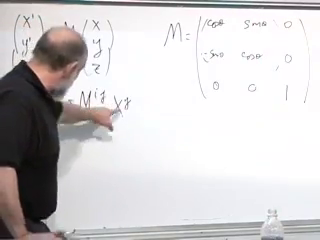
\includegraphics[width=0.82\textwidth]{lecture_05_figure_03.png}
\caption{공간 회전을 행렬 방정식과 첨자 표기법으로 각각 나타냈다.}
\lectureframe{01:00:40}
\end{figure}

\section{로런츠 행렬과 합성 속도}

\(x\)을 따른 운동에 대해, \(c=1\) 단위에서 로런츠 변환은 다음과 같다.
\begin{align}
x'&=\gamma_v(x-vt), & y'&=y,\nonumber\\
z'&=z, & t'&=\gamma_v(t-vx),
\end{align}
여기서
\begin{equation}
\gamma_v=\frac{1}{\sqrt{1-v^2}}.
\end{equation}
성분 순서를 \((x,y,z,t)\)로 쓰면 다음과 같다.
\begin{equation}
\begin{pmatrix}x'\\y'\\z'\\t'\end{pmatrix}
=
\begin{pmatrix}
\gamma_v&0&0&-\gamma_vv\\
0&1&0&0\\
0&0&1&0\\
-\gamma_vv&0&0&\gamma_v
\end{pmatrix}
\begin{pmatrix}x\\y\\z\\t\end{pmatrix}.
\label{eq:l5-lorentz-matrix}
\end{equation}

\begin{figure}[H]
\centering
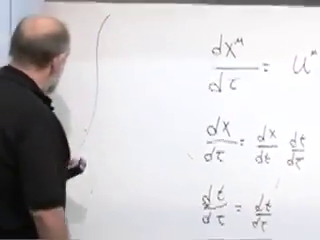
\includegraphics[width=0.82\textwidth]{lecture_05_figure_04.png}
\caption{로런츠 행렬. \(4\times4\) 성분 가운데 \(x\)와 \(t\) 성분만 서로 섞이고, \(y\)와 \(z\)는 변하지 않는다.}
\lectureframe{01:04:40}
\end{figure}

이제 행렬 곱셈으로 물리적 질문에 답해 보자. 한 관찰자가 우리에 대해 속도 \(v\)로 움직이고, 세 번째 관찰자가 그 관찰자에 대해 속도 \(u\)로 같은 축을 따라 움직인다고 하자. 뉴턴 역학에서는 \(w=u+v\)이 되어, 속도 \(3c/4\) 두 개가 합쳐져 \(3c/2\)가 될 수 있다. 상대론에서는 다른 법칙이 나와야 한다.

부스트에서 관련된 부분은 \(2\times2\) 행렬이다.
\begin{equation}
B(v)=\gamma_v
\begin{pmatrix}1&-v\\-v&1\end{pmatrix}.
\end{equation}
두 부스트를 합성하면
\begin{align}
B(u)B(v)
&=\gamma_u\gamma_v
\begin{pmatrix}1&-u\\-u&1\end{pmatrix}
\begin{pmatrix}1&-v\\-v&1\end{pmatrix}\nonumber\\
&=\gamma_u\gamma_v
\begin{pmatrix}
1+uv&-(u+v)\\
-(u+v)&1+uv
\end{pmatrix}.
\label{eq:l5-composed-boost}
\end{align}
비대각 성분과 대각 성분의 비로 결과 부스트의 속도를 구할 수 있다.
\begin{equation}
w=\frac{u+v}{1+uv}
\qquad(c=1).
\end{equation}
차원을 되살리면,
\begin{equation}
w=\frac{u+v}{1+uv/c^2}.
\label{eq:l5-velocity-addition}
\end{equation}

\begin{figure}[H]
\centering
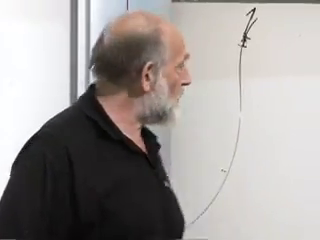
\includegraphics[width=0.82\textwidth]{lecture_05_figure_05.png}
\caption{부스트를 합성한 행렬과 자연 단위계에서의 속도 \(w=(u+v)/(1+uv)\).}
\lectureframe{01:15:35}
\end{figure}

\(u\)와 \(v\)가 각각 \(c\)에 가까우면 분자는 \(2c\)에 가까워지고 분모는 \(2\)에 가까워지므로, \(w\)는 \(2c\)가 아니라 \(c\)에 가까워진다. 더 일반적으로 식 ~\eqref{eq:l5-velocity-addition}은 광속보다 작은 입력 속도들을 광속보다 작은 결과 속도로 보낸다. 행렬 곱셈에 속도 제한이 자동으로 반영된 것이다.

\section{4-벡터와 보통 속도의 한계}

4-벡터란 네 성분이 시공간 좌표와 같은 방식으로 회전과 로런츠 부스트에 따라 변환하는 임의의 대상을 말한다. \(V^\mu\)가 4-벡터라면, 우리의 부호 관례에서
\begin{equation}
V_\mu=(-V^1,-V^2,-V^3,V^0),
\end{equation}
불변 노름은 다음과 같다.
\begin{equation}
V_\mu V^\mu=(V^0)^2-(V^1)^2-(V^2)^2-(V^3)^2.
\end{equation}
두 4-벡터 \(V^\mu\)와 \(W^\mu\)의 수축량
\begin{equation}
W_\mu V^\mu
=W^0V^0-W^1V^1-W^2V^2-W^3V^3
\end{equation}
도 마찬가지로 불변이다. 기준계에 따라 성분은 변하지만 수축량은 변하지 않는다.

보통 속도는 성분이 세 개뿐이다.
\begin{equation}
\mathbf v=\left(\frac{dx}{dt},\frac{dy}{dt},\frac{dz}{dt}\right).
\end{equation}
\(dt/dt=1\)를 덧붙여도 유용한 4-벡터가 되지는 않는다. 네 번째 성분은 자명하고, 이렇게 얻은 대상은 로런츠 변환 아래에서 선형적으로 변환하지 않는다. 좌표 시간 \(t\)은 기준계마다 달라지므로, \(t\)으로 미분하면 원하는 변환 법칙이 깨진다.

고유 시간을 쓰면 이 문제가 해결된다. 세계선을 따라 다음과 같이 정의하자.
\begin{equation}
u^\mu=\frac{dX^\mu}{d\tau}.
\label{eq:l5-four-velocity}
\end{equation}
미소량 \(dX^\mu\)는 4-벡터이고 \(d\tau\)는 불변이므로, 이 둘의 비는 4-벡터다. ``고유''라는 말은 분모에 있는 시계를 가리킨다.

연쇄 법칙으로 이 대상을 보통 속도와 관련지을 수 있다.
\begin{equation}
\frac{dx}{d\tau}=\frac{dx}{dt}\frac{dt}{d\tau},
\end{equation}
\(y\)와 \(z\)에 대해서도 마찬가지다. 식 ~\eqref{eq:l5-proper-time}에서
\begin{align}
\left(\frac{d\tau}{dt}\right)^2
&=1-\left(\frac{dx}{dt}\right)^2
    -\left(\frac{dy}{dt}\right)^2
    -\left(\frac{dz}{dt}\right)^2\nonumber\\
&=1-v^2
\qquad(c=1),
\end{align}
따라서
\begin{equation}
\frac{dt}{d\tau}=\gamma_v=\frac{1}{\sqrt{1-v^2}}.
\end{equation}
네 성분은 다음과 같다.
\begin{equation}
u^i=\gamma_v v^i,
\qquad
u^0=\gamma_v
\qquad(c=1).
\label{eq:l5-four-velocity-components}
\end{equation}
속도가 낮으면 \(u^i\simeq v^i\)이고 \(u^0\simeq1\)이다. 빛의 속도에 가까워지면 \(\gamma_v\)는 한없이 커지고 고유 속도는 보통 속도와 크게 달라진다.

\begin{figure}[H]
\centering
\includegraphics[width=0.82\textwidth]{lecture_05_figure_06.png}
\caption{고유 속도의 네 성분을 보통 속도와 로런츠 인자로 나타냈다.}
\lectureframe{01:34:40}
\end{figure}

보통 단위를 되살리고 \(X^0=ct\)를 사용하면, 여기서 쓰는 공간 성분 우선 순서에 따른 표준형은 다음과 같다.
\begin{equation}
U^\mu=(\gamma_v\mathbf v,\gamma_v c)
\end{equation}
불변 노름은
\begin{equation}
U_\mu U^\mu=c^2.
\end{equation}
따라서 모든 질량을 가진 입자는 공간 속도가 기준계에 따라 달라지더라도 크기가 같은 불변 노름의 4-속도를 갖는다.

\section{세계선의 접선}

식 ~\eqref{eq:l5-four-velocity}을 이해하는 데 익숙한 유클리드 공간의 예를 들 수 있다. 보통의 3차원 공간에서 곡선을 따라가면,
\begin{equation}
ds^2=dx^2+dy^2+dz^2.
\end{equation}
미소 변위 \((dx,dy,dz)\)는 곡선을 따라 향하지만 단위 벡터는 아니다. 이를 호의 길이로 나누면
\begin{equation}
\mathbf T=
\left(\frac{dx}{ds},\frac{dy}{ds},\frac{dz}{ds}\right),
\qquad
\mathbf T\cdot\mathbf T=1.
\end{equation}
상대론적 구성도 같은 생각을 따른다. 다만 유클리드 호의 길이 대신 고유 시간을 쓴다. 벡터 \(u^\mu=dX^\mu/d\tau\)는 세계선의 접선이다.

\begin{figure}[H]
\centering
\includegraphics[width=0.82\textwidth]{lecture_05_figure_07.png}
\caption{유클리드 공간에서 접선 벡터를 만드는 과정. 미소 변위 벡터를 호의 길이 요소 \(ds\)로 나눈다. 시간꼴 세계선을 따라서는 고유 시간이 이에 상응하는 역할을 한다.}
\lectureframe{01:39:30}
\end{figure}

\begin{classroomqa}
\audiencequestion{\(c=1\)라면 고유 시간과 고유 거리는 같은 건가요?}
\lecturerresponse{\(c=1\)로 두면 시간과 거리를 같은 단위로 나타낼 수 있지만, 시공간 기하학의 마이너스 부호가 사라지는 것은 아니다. 유클리드 유추에서 \(s\)은 공간 곡선을 따라 잰 보통 거리다. 시간꼴 세계선에서 \(\tau\)은 시계가 측정한 경과 시간이다. 구성은 서로 유사하지만 기하학은 다르다.}
\end{classroomqa}

한 번 더 미분하면 고유 가속도가 정의된다.
\begin{equation}
a^\mu=\frac{du^\mu}{d\tau}.
\end{equation}
뉴턴의 제2법칙을 상대론적으로 일반화할 때 \(d^2\mathbf x/dt^2\) 대신 써야 하는 물리량이 바로 이것이다. \(u_\mu u^\mu\)가 상수이므로,
\begin{equation}
\frac{d}{d\tau}(u_\mu u^\mu)=2u_\mu a^\mu=0,
\end{equation}
따라서 4-가속도는 민코프스키 내적에서 4-속도와 직교한다.\editorialnote{직교성은 불변 노름에서 바로 따라 나오며, 정의에서 얻는 다음 수학적 귀결로 여기에 덧붙였다.}

\section{4-운동량과 에너지}

운동량은 충돌과 붕괴에서 보존되므로 마지막 예로 살펴보자. 입자는 고정된 고유 질량 \(m\)을 가지며, 이를 정지 질량이라고도 한다. 이 질량은 속도에 따라 변하지 않는다. 상대론적 운동량은 이 고정된 질량과 4-속도의 곱이다.
\begin{equation}
p^\mu=mu^\mu.
\label{eq:l5-four-momentum}
\end{equation}
\(c=1\) 단위에서는,
\begin{equation}
p^i=\gamma_v m v^i,
\qquad
p^0=\gamma_v m.
\end{equation}
속도가 낮아 \(\gamma_v\simeq1\)이면 공간 성분은 뉴턴 역학의 운동량 \(m\mathbf v\)로 줄어든다. 고속에서는 이 성분들이 \(m\mathbf v\)보다 더 빠르게 커진다.

시간 성분은 에너지다. 보통 단위를 쓰고 \(X^0=ct\)로 두면,
\begin{equation}
P^\mu=(\mathbf p,E/c)
=(\gamma_v m\mathbf v,\gamma_v mc),
\end{equation}
따라서
\begin{equation}
E=\gamma_v mc^2
=mc^2\left(1-\frac{v^2}{c^2}\right)^{-1/2}.
\label{eq:l5-relativistic-energy}
\end{equation}

보통 역학을 되찾으려면 다음과 같이 두자.
\(\epsilon=v^2/c^2\ll1\). 이항 전개를 하면
\begin{equation}
(1-\epsilon)^p=1-p\epsilon+O(\epsilon^2).
\end{equation}
\(p=-1/2\)로 두면,
\begin{align}
E
&=mc^2\left(1-\frac{v^2}{c^2}\right)^{-1/2}\nonumber\\
&=mc^2\left[1+\frac12\frac{v^2}{c^2}
  +O\!\left(\frac{v^4}{c^4}\right)\right]\nonumber\\
&=mc^2+\frac12mv^2+O\!\left(\frac{mv^4}{c^2}\right).
\label{eq:l5-energy-expansion}
\end{align}

\begin{figure}[H]
\centering
\includegraphics[width=0.82\textwidth]{lecture_05_figure_08.png}
\caption{저속에서의 상대론적 에너지 전개. 정지 에너지와 뉴턴 역학의 운동 에너지가 드러난다.}
\lectureframe{01:51:30}
\end{figure}

첫째 항인 \(mc^2\)은 정지해 있을 때도 존재한다. 입자 집합과 각 입자의 질량이 변하지 않는 뉴턴 역학 문제에서는 그 항이 운동 전후에 같은 상수를 더하므로, 익숙한 장부 계산에서는 \(\tfrac12mv^2\)만 고려한다. 상대론에 따르면 버려진 그 상수도 처음부터 물리적인 에너지였다.

따라서 에너지와 운동량은 서로 무관한 보존 법칙이 아니다. 이들은 하나의 보존 벡터를 이루는 네 성분이다. 로런츠 부스트는 이들을 서로 섞는다. 한 관찰자가 에너지라고 부르는 것의 일부는 다른 관찰자에게 운동량으로 기여하며, 그 반대도 마찬가지다. 그렇더라도 고립계의 전체 4-운동량은 모든 관성계에서 충돌이나 붕괴 전후로 같다.

이 지점에서 상대론적 역학의 문턱에 이른다. 다음으로 할 일은 고유 가속도로 힘을 표현하고, 상대론적 파동 방정식, 특히 전자기와 빛을 지배하는 방정식을 이해하는 것이다.

\chapter{불변 법칙, 4-벡터, 그리고 장 텐서}

먼저 자연이 따를 수도 있었지만 실제로는 따르지 않는 법칙을 살펴보자. 이 법칙이 성립하지 않는다는 사실은 물리 법칙을 어떻게 써야 하는지 알려준다. 같은 기준을 적용하면 먼저 좌표 성분에서 보통 벡터로, 이어서 보통 벡터에서 4-벡터로, 마지막으로 4-벡터에서 텐서로 나아가게 된다. 이 과정을 마치면 전기장과 자기장은 더 이상 서로 분리된 대상이 아니다. 두 장은 하나의 반대칭 텐서에서 서로 독립적인 여섯 성분을 이룬다.

달리 명시하지 않는 한 \(c=1\)인 단위를 사용하고, 시공간 성분의 순서를 \((1,2,3,0)=(x,y,z,t)\)로 하며, 계량 부호 규약은 \((-,-,-,+)\)로 둔다.

\section{대칭성이 잘못된 법칙의 한 예}

공간에 \(x\)축과 \(y\)축을 고정해 두자. 이제 두 입자의 \(x\)좌표가 일치할 때마다 입자들이 상호작용한다고 정해 보자. 이 상호작용으로 입자들의 운동 방향이 반대로 바뀌거나 새로운 방향으로 흩어질 수 있다. 구체적인 동역학은 중요하지 않다. 제안된 상호작용의 조건은 그저 \begin{equation}
  x_1-x_2=0,
\end{equation}이며, 아래 첨자는 좌표 성분이 아니라 입자를 가리킨다. 이 규칙에는 수학적 모순이 없다. 문제는 무엇 때문에 이 규칙을 물리적으로 타당하지 않다고 보는가이다.

\begin{classroomqa}\audiencequestion{이 규칙은 공간의 균질성을 위반하나요?}\lecturerresponse{아닙니다. 원점을 평행이동하면 두 좌표가 똑같은 양만큼 변하므로 \(x_1-x_2\)는 변하지 않습니다. 이 규칙은 특정 위치를 특별하게 취급하지 않습니다. 결함은 등방성에 있습니다. 특정 방향 하나를 특별하게 선택하기 때문입니다.}\end{classroomqa}

축을 \(90^\circ\)만큼 회전해 보자. 원래 \(x\)방향이라고 부르던 방향은 이제 \(y\)방향이므로, 같은 물리적 사건은 \(y\)좌표가 같다는 조건으로 기술된다. 일반적인 각도에서는 조건에 \(x\)와 \(y\)의 선형 결합이 들어간다. 따라서 법칙의 형태가 칠판을 어떤 방향으로 놓았는지에 따라 달라진다. 이 법칙은 평행이동에는 불변이지만 회전에는 불변이 아니다.

물리 법칙은 보통 직교 좌표계에서 가장 간단한 형태로 쓴다. 더 일반적인 좌표계를 쓸 수도 있지만, 그러면 계량과 식이 덜 간단해진다. 직교 데카르트 좌표계라는 범위 안에서는 어느 방향도 특별하게 취급해서는 안 된다.

수정 방법은 간단하다. 2차원에서는 두 좌표가 모두 일치하도록 하고, 3차원에서는 세 좌표가 모두 일치하도록 한다. \begin{equation}
  x_1=x_2,
  \qquad y_1=y_2,
  \qquad z_1=z_2.
\end{equation} 그러면 입자들은 서로 다른 직선을 따라 접근하더라도 같은 점에 도달할 때에만 상호작용할 수 있다.

\begin{classroomqa}\audiencequestion{\(z\)좌표와 시간도 일치해야 하나요?}\lecturerresponse{3차원 공간에서는 \(z\)좌표도 일치해야 합니다. 지금은 시간을 잠시 생략하지만, 공간에 관한 논의를 마치면 곧 다시 포함하겠습니다.}\end{classroomqa}

\(\boldsymbol r_a\)는 입자 \(a\)의 위치이다. 세 성분에 대한 조건은 하나의 벡터 방정식으로 나타낼 수 있다.
\begin{equation}
  \boldsymbol r_1-\boldsymbol r_2=\boldsymbol 0.
\end{equation}
어떤 회전 좌표계에서는 한 성분이 사라지지만, 다른 회전 좌표계에서는 사라지지 않을 수 있다. 벡터 전체에 대해서는 다르다. 한 좌표계에서 모든 성분이 사라지면 회전한 모든 좌표계에서도 모든 성분이 사라진다. 마찬가지로 한 좌표계에서 두 벡터가 같으면 둘 다 변환한 뒤에도 서로 같다.

\begin{figure}[H]\centering
\includegraphics[width=0.78\textwidth]{lecture_06_figure_01.png}\caption{충돌이 특정한 한 축을 따라 일치하는 것이 아니라 공간상의 일치를 뜻하게 하는 세 좌표의 등식.}\lectureframe{00:09:00}\end{figure}

벡터 방정식이 유용한 이유가 여기에 있다. 성분은 변하지만 대상 전체는 일관되게 변환된다. 전체 대상에 대해 쓴 법칙은 좌표계를 회전해도 형태를 유지할 수 있다.

\section{시공간에서의 일치}

이제 수직인 공간축을 시간으로 바꾸어 보자. 뉴턴 역학의 규칙은 두 운동 변화가 같은 시간에만 일어난다고 할 수 있다. 뉴턴 역학에서는 모든 관성 관찰자가 동시성을 공유하므로 그런 규칙이 가능하다. 특수 상대성 이론에서는 이 규칙이 특정 기준계를 선택한다. 한 기준계에서 동시인 사건들이 다른 기준계에서는 동시가 아닐 수 있다.

공간 좌표만 같다고 요구해도 나을 것이 없다. 시공간 변위는 공간 성분은 사라지고 시간 성분은 남는다.
\begin{equation}
  \Delta X^\mu=(0,0,0,\Delta t),
\end{equation}
부스트는 \(\Delta t\)와 공간 성분을 서로 섞는다. 불변인 국소적 진술은 두 운동 변화가 같은 사건에서 일어난다는 것이다. 따라서 단순한 충돌이 일어나려면 다음 조건이 필요하다.
\begin{equation}
  X_1^\mu=X_2^\mu,
  \qquad\text{or}\qquad
  X_1^\mu-X_2^\mu=0.
\end{equation}
네 좌표가 모두 일치한다. 즉 입자들은 같은 시각에 같은 위치를 차지한다.

충돌의 예는 물리학을 기술하는 일반적인 원칙을 보여준다. 모든 항을 한쪽에 모아 완전한 4-벡터를 0과 같게 두거나, 완전한 4-벡터 하나를 다른 하나와 같게 둘 수 있다. 4-벡터의 서로 연결되지 않은 일부만 같게 두는 것만으로는 로런츠 불변인 진술이 되지 않는다.

\section{부스트, 회전, 행렬 표기}

4-벡터란 시공간 변위와 같은 방식으로 변환되는 대상이다. 이 정의를 유용하게 쓰려면 먼저 좌표 자체의 변환을 떠올려야 한다. \(x\)방향으로 속력 \(v\)인 부스트의 경우, \begin{align}
  x'&=\gamma(x-vt), & y'&=y, & z'&=z,
  & t'&=\gamma(t-vx),                                      \label{eq:l6-boost}
\end{align} 여기서 \begin{equation}
  \gamma(v)=\frac{1}{\sqrt{1-v^2}}.
\end{equation}

\begin{classroomqa}\audiencequestion{이 식들에서는 빛의 속도를 1로 둔 건가요?}\lecturerresponse{그렇습니다. 단위를 복원하려면 \(X^0=ct\)로 놓고, \(1-v^2\)를 \(1-v^2/c^2\)로 바꾸며, 공간--시간 혼합항에 해당하는 \(c\)의 인자도 복원하면 됩니다.}\end{classroomqa}

\(z\)축 주위의 회전은 \(x\)와 \(y\)를 서로 섞고, \(z\)와 \(t\)는 그대로 둔다. \begin{equation}
\begin{pmatrix}
  x'\\ y'\\ z'\\ t'
\end{pmatrix}
=
\begin{pmatrix}
  \cos\theta & \sin\theta & 0 & 0\\
  -\sin\theta & \cos\theta & 0 & 0\\
  0 & 0 & 1 & 0\\
  0 & 0 & 0 & 1
\end{pmatrix}
\begin{pmatrix}
  x\\ y\\ z\\ t
\end{pmatrix}.
\end{equation} 영점도 표시할 필요가 있다. 변환된 좌표에 어떤 성분이 들어가지 않는지 분명하게 보여주기 때문이다. 같은 성분 순서로 쓰면 식~\eqref{eq:l6-boost}의 부스트는 다음과 같다. \begin{equation}
\begin{pmatrix}
  x'\\ y'\\ z'\\ t'
\end{pmatrix}
=
\begin{pmatrix}
  \gamma & 0 & 0 & -\gamma v\\
  0 & 1 & 0 & 0\\
  0 & 0 & 1 & 0\\
  -\gamma v & 0 & 0 & \gamma
\end{pmatrix}
\begin{pmatrix}
  x\\ y\\ z\\ t
\end{pmatrix}.
\end{equation}

회전과 부스트는 행렬 곱셈으로 합성할 수 있다. 원래 \(x\)축과 나란하지 않은 방향으로 부스트하려면, 그 방향이 \(x\)축과 나란해지도록 회전한 뒤 부스트를 적용하고 필요에 따라 다시 회전하면 된다. 이런 기본 행렬들의 곱으로 더 일반적인 로런츠 변환을 만들 수 있다.

\begin{classroomqa}\audiencequestion{먼저 회전한 뒤 부스트하는 것과 먼저 부스트한 뒤 회전하는 것은 차이가 있나요?}\lecturerresponse{있습니다. 첫 번째 연산을 거치면 두 번째 연산이 작용하는 축이 바뀝니다. 따라서 두 행렬 곱은 같지 않을 수 있고, 연산 순서가 중요합니다.}\end{classroomqa}

이 모든 선형 변환을 한꺼번에 다음과 같이 쓸 수 있다. \begin{equation}
  X'^{\mu}=\Lambda^{\mu}{}_{\nu}X^{\nu}.                  \label{eq:l6-vector-transform}
\end{equation} 반복되는 첨자 \(\nu\)에 대해서는 \(1,2,3,0\)에 걸쳐 합한다. 이는 행렬 곱셈에서 행과 열의 원소를 곱해 더하는 통상적인 계산을 첨자 표기로 나타낸 것이다.

\begin{figure}[H]\centering
\includegraphics[width=0.78\textwidth]{lecture_06_figure_02.png}\caption{열벡터 형태로 쓰기 전의 로런츠 변환 첨자 표기.}\lectureframe{00:31:55}\end{figure}

식~\eqref{eq:l6-vector-transform}은 일반적인 반변 4-벡터의 정의이기도 하다. \(A^\mu\)가 그런 벡터라면 다음과 같이 변환된다. \begin{equation}
  A'^{\mu}=\Lambda^{\mu}{}_{\nu}A^{\nu}.
\end{equation} 네 성분이 위치를 나타낼 필요는 없다. 이 대상이 4-벡터인 까닭은 그 변환 법칙에 있다.

\section{스칼라, 계량, 불변 곱}

4-벡터를 더 다루기 전에 한 걸음 물러나 스칼라라는 더 간단한 개념을 살펴보면 도움이 된다. 공간상의 특정 지점에서의 온도는 스칼라이며, 두 특정 지점 사이의 거리도 스칼라이다. 각각은 축의 방향과 무관한 하나의 수이다. 일부러 우스꽝스럽게, 센티미터로 잰 거리가 화씨 온도로 잰 실내 온도와 같다고 주장할 수도 있다. 물리적으로 의미 있는 주장은 아니지만, 양변이 모두 회전 스칼라이므로 축을 어떻게 돌리든 그 주장의 참과 거짓은 달라지지 않는다.

벡터의 성분은 스칼라가 아니다. 따라서 성분을 스칼라로 결합하는 체계적인 방법이 필요하다. 일반적인 반변 4-벡터를 다음과 같이 쓰자. \begin{equation}
  A^\mu=(A^1,A^2,A^3,A^0).
\end{equation} 공변 성분은 같은 기하학적 대상을 아래 첨자로 나타낸 것이다. 우리가 쓰는 부호 규약에서는 민코프스키 계량을 사용해 다음과 같이 구한다. \begin{equation}
  A_\mu=\eta_{\mu\nu}A^\nu,
  \qquad
  \eta_{\mu\nu}=
  \begin{pmatrix}
    -1&0&0&0\\
    0&-1&0&0\\
    0&0&-1&0\\
    0&0&0&1
  \end{pmatrix},                                          \label{eq:l6-metric}
\end{equation} 따라서 \begin{equation}
  A_\mu=(-A^1,-A^2,-A^3,A^0).
\end{equation}

\begin{classroomqa}\audiencequestion{칠판에 쓴 첨자와 부호 둘이 서로 맞지 않나요?}\lecturerresponse{맞습니다. 표시된 열벡터의 공간 성분에는 해당하는 음의 부호가 필요합니다. 첨자를 내리는 식에서 계량 \(\eta_{\mu\nu}\)을 곱하기 전 오른쪽 성분들의 첨자는 위쪽이어야 합니다. 시간 성분의 첨자는 \(0\)이지 \(4\)가 아닙니다.}\end{classroomqa}

\begin{figure}[H]\centering
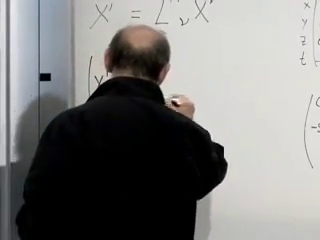
\includegraphics[width=0.8\textwidth]{lecture_06_figure_03.png}\caption{반변 성분과 공변 성분, 계량 행렬, 그리고 불변 수축의 시작.}\lectureframe{00:45:00}\end{figure}

첨자를 내리는 것은 단순한 표기상의 장식이 아니다. 로런츠 불변 노름에 필요한 부호를 반영한다. \begin{align}
  A_\mu A^\mu
  &=-(A^1)^2-(A^2)^2-(A^3)^2+(A^0)^2,                    \label{eq:l6-norm}\\
  X_\mu X^\mu
  &=t^2-x^2-y^2-z^2.
\end{align} 두 번째 식은 원점에서부터의 불변 시공간 간격이다. \(A^\mu\)가 \(X^\mu\)와 같은 방식으로 변환하므로 그 수축은 불변이다.

이 표기는 유용한 계산 규칙도 알려준다. 합산되는 첨자는 위에 한 번, 아래에 한 번 나타난다. 예를 들면 다음과 같다. \begin{equation}
  A_\mu A^\mu
  =\eta_{\mu\nu}A^\mu A^\nu.
\end{equation} 합산 첨자, 즉 더미 첨자의 이름은 양을 바꾸지 않고 바꿀 수 있다.

\begin{classroomqa}\audiencequestion{이 벡터 중 하나를 행으로, 다른 하나를 열로 봐야 하나요? 그리고 순서가 중요한가요?}\lecturerresponse{현재 계산에서는 첨자가 붙은 양을 성분으로 보고 계량으로 수축하면 됩니다. 논의를 행과 열의 연산자 대수로 바꿀 필요는 없습니다. 이들은 보통 수이므로 순서는 중요하지 않습니다. 교환하지 않는 연산자라면 더 주의해야 하지만, 여기서는 그런 내용을 다루지 않습니다.}\end{classroomqa}

같은 구성으로 서로 다른 두 4-벡터 사이의 내적을 얻을 수 있다. \begin{equation}
  A\mathbin{\cdot}B=A_\mu B^\mu=A^\mu B_\mu.
\end{equation} 로런츠 행렬을 명시적으로 쓰지 않고도 이 내적이 불변임을 보일 수 있다. \(A+B\)와 \(A-B\)가 4-벡터이므로 두 제곱 노름은 모두 불변이다. \begin{align}
  (A+B)^2&=A^2+B^2+2A\mathbin{\cdot}B,\\
  (A-B)^2&=A^2+B^2-2A\mathbin{\cdot}B.
\end{align} 두 식을 빼면 다음을 얻는다. \begin{equation}
  (A+B)^2-(A-B)^2=4A\mathbin{\cdot}B,                    \label{eq:l6-polarization}
\end{equation} 따라서 \(A\mathbin{\cdot}B\)도 불변이다. 인수 4는 전개에서 바로 나온다.\editorialnote{칠판의 논증은 이 편극 항등식을 보여준다. 인수를 직접 적어 두면 말로 설명한 소거 과정이 모호하지 않다.}

\begin{figure}[H]\centering
\includegraphics[width=0.8\textwidth]{lecture_06_figure_04.png}\caption{서로 다른 4-벡터의 내적을 분리해 구하는 데 쓰인 두 불변 제곱식.}\lectureframe{00:52:20}\end{figure}

불변량은 물리 법칙에 자연스럽게 들어간다. 고립된 성분과 달리 기준계가 바뀌어도 같은 값을 유지하기 때문이다.

\section{고유 속도와 4-운동량}

입자의 세계선 위에서 서로 이웃한 두 사건을 생각하자. 두 사건의 간격은 미소 4-벡터이다. \begin{equation}
  dX^\mu=(dx,dy,dz,dt).
\end{equation} 시간꼴 세계선에 대해서는 고유시간을 다음과 같이 정의한다. \begin{equation}
  d\tau^2=dX_\mu dX^\mu
  =dt^2-dx^2-dy^2-dz^2.                                  \label{eq:l6-proper-time}
\end{equation} 고유 4-속도는 다음과 같다. \begin{equation}
  U^\mu=\frac{dX^\mu}{d\tau}.                            \label{eq:l6-four-velocity}
\end{equation} 이는 특정 기준계의 좌표 시간이 아니라 입자 자신의 고유시간에 대한 시공간 위치의 변화율이다.

\(U^\mu\)에는 성분이 네 개 있지만 독립적인 성분은 세 개뿐이다. 식~\eqref{eq:l6-proper-time}을 \(d\tau^2\)으로 나누면 다음을 얻는다. \begin{equation}
  U_\mu U^\mu=1.
\end{equation} 따라서 4-속도는 단위 시간꼴 벡터이다. 미래 방향을 택하면 시간 성분의 부호가 정해진다.

\begin{classroomqa}\audiencequestion{\(c\)보다 훨씬 느린 속도에서는 4-속도가 보통 속도로 줄어드나요?}\lecturerresponse{공간 성분 세 개는 보통 속도에 가까워지고, 시간 성분은 \(c=1\) 단위에서 1에 가까워집니다. 연쇄 법칙을 적용하고 \(dt/d\tau\)을 계산하면 이 관계를 얻습니다.}\end{classroomqa}

각 공간 성분에 대해 다음이 성립한다. \begin{equation}
  U^i=\frac{dx^i}{d\tau}
     =\frac{dx^i}{dt}\frac{dt}{d\tau}
     =v^i\frac{dt}{d\tau}.
\end{equation} 식~\eqref{eq:l6-proper-time}을 \(dt^2\)으로 나누면 다음과 같다. \begin{equation}
  \left(\frac{d\tau}{dt}\right)^2
  =1-v_x^2-v_y^2-v_z^2
  =1-\boldsymbol v^2.
\end{equation} 따라서 \begin{equation}
  \frac{dt}{d\tau}=\frac{1}{\sqrt{1-\boldsymbol v^2}}
  =\gamma(\lvert\boldsymbol v\rvert),
\end{equation}이고, \begin{equation}
  U^\mu=(\gamma v_x,\gamma v_y,\gamma v_z,\gamma).
                                                                  \label{eq:l6-u-components}
\end{equation}

\begin{figure}[H]\centering
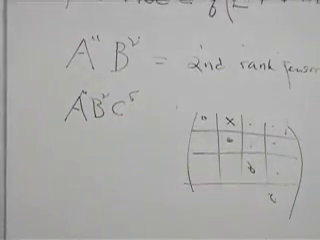
\includegraphics[width=0.8\textwidth]{lecture_06_figure_05.png}\caption{고유시간 계산으로 \(dt/d\tau=\gamma\)을 구하고 고유 속도와 보통 속도의 관계를 나타낸다.}\lectureframe{01:02:00}\end{figure}

\begin{classroomqa}\audiencequestion{\(dx^2/dt^2\)는 이계도함수를 뜻하나요? 벡터를 제곱하면 교차항이 생겨야 하지 않나요?}\lecturerresponse{여기서는 일계도함수의 제곱인 \((dx/dt)^2\)를 뜻합니다. 또 \(\boldsymbol v^2\)은 유클리드 내적 \(v_x^2+v_y^2+v_z^2\)을 뜻하지 형식적인 합 \(v_x+v_y+v_z\)의 제곱을 뜻하지 않으므로 교차항은 없습니다.}\end{classroomqa}

\begin{classroomqa}\audiencequestion{\(v\)는 \(\gamma(v)\)에서 두 기준계 사이의 상대 속도인가요, 아니면 입자의 속도인가요?}\lecturerresponse{여기서는 선택한 기준계에서 본 입자의 속도입니다. 함수 \(\gamma(v)=1/\sqrt{1-v^2}\)는 어떤 속도에 대해서도 계산할 수 있습니다. 부스트에서는 기준계 사이의 상대 속도를 대입하고, 4-속도에서는 입자의 속도를 대입합니다.}\end{classroomqa}

\(v\ll1\)이면 \(\gamma\simeq1\)이므로 \(U^\mu\)의 공간 성분은 \(\boldsymbol v\)에 가까워지고 \(U^0\)은 1에 가까워진다. 보통 속도가 빛의 속도에 가까워지면 \(\gamma\)는 커지고 사차원 속도의 0이 아닌 모든 성분은 한없이 커진다.

\begin{classroomqa}\audiencequestion{\(U^0\)는 1에 가까운 수가 아니라 속도의 단위를 가져야 하지 않나요?}\lecturerresponse{\(c\)를 1로 두면서 단위가 사라졌습니다. \(X^0=ct\)를 사용하면 \(U^\mu=(\gamma\boldsymbol v,\gamma c)\)이므로 시간 성분은 \(c\)에 가까워지고 \(U_\mu U^\mu=c^2\)가 됩니다.}\end{classroomqa}

정지 질량이 \(m\)인 입자의 4-운동량을 다음과 같이 정의하자. \begin{equation}
  P^\mu=mU^\mu.
\end{equation} 자연 단위계에서는 \begin{equation}
  P^\mu=(\gamma m\boldsymbol v,\gamma m).
\end{equation} 저속에서 처음 세 성분은 뉴턴 역학의 운동량 \(m\boldsymbol v\)에 가까워진다. 단위를 복원하면 다음과 같다. \begin{equation}
  P^\mu=(\gamma m\boldsymbol v,E/c),
  \qquad E=\gamma mc^2,
\end{equation} 따라서 \begin{equation}
  E=mc^2+\frac{1}{2}m\boldsymbol v^2+O(mv^4/c^2).
\end{equation} 시간 성분은 \(c=1\) 단위계에서 에너지이며, 네 성분 모두에 운동량 단위를 부여하면 에너지를 \(c\)로 나눈 값이다.

\begin{classroomqa}\audiencequestion{\(\boldsymbol v\)의 끝에 네 번째 성분을 붙인 것 자체가 4-벡터인가요?}\lecturerresponse{아닙니다. 보통 3-속도는 4-벡터처럼 변환되지 않습니다. 인자 \(\gamma\)와 고유시간을 이용한 정의가 필수입니다. 4-벡터는 \(U^\mu\)이지 \(\boldsymbol v\)가 아닙니다.}\end{classroomqa}

\section{전기장과 자기장이 서로 섞여야 하는 이유}

이제 상대성 이론을 잠시 쉬어 간다. 아인슈타인 이전의 운동 방정식에서 시작해, 모든 관성 기준계에서 성립하려면 이 방정식을 어떻게 다시 구성해야 하는지 살펴보자. 보통 가속도는 보통 속도의 시간 미분이다. 이에 대응하는 4차원 양은 자연스럽게 다음과 같다. \begin{equation}
  A^\mu=\frac{dU^\mu}{d\tau}.
\end{equation} 저속에서는 그 공간 성분이 보통 가속도에 가까워진다. 완전한 상대론적 방정식은 뒤로 미루고, 먼저 옛 힘 법칙을 살펴보자.

전기장과 자기장 속의 전하 \(q\)에 대해 \begin{equation}
  \boldsymbol F=m\boldsymbol a
  =q\left(\boldsymbol E+\boldsymbol v\times\boldsymbol B\right).
                                                                  \label{eq:l6-lorentz-force}
\end{equation} 전기력 항은 입자 속도와 무관하지만 자기력 항은 그렇지 않다.

\begin{figure}[H]\centering
\includegraphics[width=0.8\textwidth]{lecture_06_figure_06.png}\caption{\(\boldsymbol E\)과 \(\boldsymbol B\)를 결합해야 하는 이유가 되는 상대론 이전의 로런츠 힘 법칙.}\lectureframe{01:18:20}\end{figure}

관측자가 전기장은 없고 자기장과 움직이는 전하는 있다고 본다고 하자. 전하는 자기력을 받는다. 그러나 전하의 순간 정지 좌표계에서는 \(\boldsymbol v=0\)이므로 식~\eqref{eq:l6-lorentz-force}의 자기 항은 사라진다. 좌표계가 바뀌었다고 해서 물리적 세계선이 관성 운동을 하게 된 것은 아니다. 따라서 새 좌표계에서 힘에는 전기력에 해당하는 항이 포함되어야 한다. 더 정확히 말하면, 관성 좌표계 사이의 변환으로 4-가속도를 0으로 만들 수는 없다. 다만 보통의 3-가속도와 그 성분은 변환된다.
\editorialnote{4-가속도에 관한 이 진술은 강의실 논증을 불변인 형태로 나타내며, 보통의 3-가속도 자체를 좌표계에 무관한 양으로 취급하지 않도록 해 준다.}

따라서 전기장과 자기장은 서로 변환되어야 한다. 두 장을 합치면 성분이 여섯 개이므로 하나의 스칼라도, 하나의 4-벡터도 아니다. 새로운 변환 대상을 도입해야 한다.

\section{텐서: 첨자마다 하나씩 변환}

스칼라는 계수가 0인 텐서라고 부를 수 있으며 첨자가 없다. 4-벡터는 계수가 1인 텐서이며, 네 가지 값을 가질 수 있는 첨자 하나를 갖는다. 가장 간단한 계수 2의 예는 다음과 같은 곱이다. \begin{equation}
  A^\mu B^\nu.
\end{equation} 각 첨자는 네 가지 값을 가지므로 이 대상은 \(4^2=16\)개의 성분을 가지며, \(4\times4\) 배열로 나타낼 수 있다. 세 벡터의 곱 \begin{equation}
  A^\mu B^\nu C^\sigma,
\end{equation}은 \(4^3=64\)개의 성분을 가지는 계수 3 텐서이다. 더 높은 계수에서도 이 패턴이 이어진다. 이름보다 중요한 것은 대상을 정의하는 규칙이다.

다음과 같다고 하자. \begin{equation}
  A'^{\mu}=\Lambda^\mu{}_{\nu}A^\nu,
  \qquad
  B'^{\sigma}=\Lambda^\sigma{}_{\tau}B^\tau,
\end{equation} 그러면 그 곱은 다음과 같이 변환된다. \begin{equation}
  A'^{\mu}B'^{\sigma}
  =\Lambda^\mu{}_{\nu}\Lambda^\sigma{}_{\tau}
   A^\nu B^\tau.
\end{equation} 이로부터 반변 계수 2 텐서의 정의 법칙을 얻는다. \begin{equation}
  T'^{\mu\sigma}
  =\Lambda^\mu{}_{\nu}\Lambda^\sigma{}_{\tau}T^{\nu\tau}.
                                                                  \label{eq:l6-tensor-transform}
\end{equation} 각 첨자마다 로런츠 행렬 하나가 들어간다. 반복되는 \(\nu\)와 \(\tau\)에 대해서는 합산하고, 열린 첨자 \(\mu\)와 \(\sigma\)는 프라임 기준계에서 계산하는 성분을 나타낸다.

\begin{figure}[H]\centering
\includegraphics[width=0.82\textwidth]{lecture_06_figure_07.png}\caption{두 벡터의 변환과 그에 따른 계수 2 텐서의 두 행렬 변환 법칙.}\lectureframe{01:27:15}\end{figure}

텐서가 반드시 벡터들의 단일 곱일 필요는 없다. \(A^\mu B^\nu\)와 \(A^\nu B^\mu\)는 모두 텐서 변환 법칙을 따르며, 이들의 합이나 다음과 같은 합도 마찬가지다. \begin{equation}
  A^\mu B^\nu+C^\mu D^\nu.
\end{equation} 정의는 특정한 인수분해가 아니라 변환 법칙이다. 계수 3 텐서에는 로런츠 행렬이 하나 더 붙으며, 그 이상의 계수에서도 같은 방식으로 이어진다.

\section{대칭 텐서와 반대칭 텐서}

계수 2 텐서 가운데 두 종류가 특히 유용하다. 대칭 텐서는 다음을 만족한다. \begin{equation}
  T^{\mu\nu}=T^{\nu\mu},
\end{equation} 따라서 대각선을 사이에 두고 마주 보는 성분은 서로 같다. 대각 성분 네 개와 대각선 한쪽의 성분 여섯 개로 나머지를 정할 수 있으므로, 독립 성분은 \begin{equation}
  4+6=10
\end{equation}개이다.

반대칭 텐서는 다음 조건을 만족한다.
\begin{equation}
  T^{\mu\nu}=-T^{\nu\mu}.                                \label{eq:l6-antisymmetry}
\end{equation}
\(\mu=\nu\)를 식~\eqref{eq:l6-antisymmetry}에 대입하면 \(T^{\mu\mu}=-T^{\mu\mu}\)이므로 모든 대각 성분은 0이다. 삼각형 모양의 한쪽 절반에 있는 여섯 성분으로 부호만 바꾸어 반대쪽 나머지 여섯 성분을 정할 수 있다. 따라서 독립 성분은 정확히 여섯 개이다.

\begin{figure}[H]
\centering
\includegraphics[width=0.82\textwidth]{lecture_06_figure_08.png}
\caption{완성된 반대칭 \(4\times4\) 배열: 대각선 원소는 0이고, 대각선을 기준으로 서로 마주 보는 원소들의 부호는 반대이다.}
\lectureframe{01:34:25}
\end{figure}

이 개수가 단서다. 전기장의 세 성분과 자기장의 세 성분을 하나의 반대칭 계수 2 텐서에 담을 수 있다.

\section{전자기장 텐서}

시공간 첨자를 행과 열에 \((1,2,3,0)=(x,y,z,t)\)의 순서로 배치하자. 칠판에 쓴 배열은 다음과 같다. \begin{equation}
  F_{\mu\nu}=
  \begin{pmatrix}
    0    & -B_3 & B_2  & E_1\\
    B_3  & 0    & -B_1 & E_2\\
    -B_2 & B_1  & 0    & E_3\\
    -E_1 & -E_2 & -E_3 & 0
  \end{pmatrix}.                                         \label{eq:l6-field-tensor}
\end{equation} 순수한 공간 첨자가 붙은 성분에는 자기장이 들어가고, 공간 첨자 하나와 시간 첨자 하나가 붙은 성분에는 전기장이 들어간다. 반대칭성에 따라 위쪽 삼각형의 성분을 알면 아래쪽 삼각형의 성분도 정해진다.

\begin{classroomqa}\audiencequestion{자기장 성분은 모두 음수인가요? 첨자가 \(x,y,z\)에 대응하나요?}\lecturerresponse{위쪽 공간 삼각형에서 부호는 다음과 같이 번갈아 나타납니다. \(-B_3,+B_2,-B_1\) 첨자 \(1,2,3\)는 \(x,y,z\)에 대응하고, 첨자 \(0\)는 시간을 나타냅니다. 대각선을 사이에 두고 반사하면 모든 부호가 바뀝니다.}\end{classroomqa}

\begin{figure}[H]\centering
\includegraphics[width=0.82\textwidth]{lecture_06_figure_09.png}\caption{공간 성분을 먼저 쓰는 강의의 성분 순서로 완성한 전자기장 텐서.}\lectureframe{01:41:05}\end{figure}

표기법은 보통 일반적인 \(T_{\mu\nu}\)가 아니라 \(F_{\mu\nu}\)로 쓴다. 강연자는 이 문자가 패러데이를 가리킬 수도 있다고 추측하지만, 표기의 유래는 모른다고 분명히 말한다. 여기서 중요한 것은 문자의 유래에 관한 추측이 아니라 텐서의 반대칭성과 여섯 개의 장 성분이다.

\begin{classroomqa}\audiencequestion{각 행렬 성분은 표시된 좌표 평면에서의 장의 세기를 나타내나요?}\lecturerresponse{각 성분은 전자기장 텐서의 성분입니다. 시간 첨자가 들어가는 성분은 전기 성분이고, 공간--공간 성분은 자기 성분을 나타냅니다.}\end{classroomqa}

시간 첨자가 붙은 행과 열을 분리해 두면, 나머지 \(3\times3\) 반대칭 블록은 자기장에 해당한다. 독립 성분은 다음 순환 관계로 기억할 수 있다.
\begin{equation}
  F_{12}=-B_3,
  \qquad F_{23}=-B_1,
  \qquad F_{31}=-B_2.                                   \label{eq:l6-magnetic-cycle}
\end{equation}
첫 번째 관계에서 시작해 모든 첨자를 \(1\to2\to3\to1\) 순서로 차례로 바꾸면 된다. 이를 동등하게 다음과 같이 쓸 수 있다.
\begin{equation}
  F_{ij}=-\epsilon_{ijk}B_k,
\end{equation}
여기서 \(\epsilon_{123}=+1\)이다.\editorialnote{레비--치비타 공식은 칠판에서 명시적으로 전개한 순환 규칙을 간결하게 나타내는 표준형이다.}

\begin{figure}[H]\centering
\includegraphics[width=0.82\textwidth]{lecture_06_figure_10.png}\caption{반대칭 텐서에서 자기장을 나타내는 공간 성분들의 순환 관계.}\lectureframe{01:46:20}\end{figure}

전기장의 대응 관계는 더 직접적이다. \begin{equation}
  E_1=F_{10},
  \qquad E_2=F_{20},
  \qquad E_3=F_{30}.
\end{equation}

따라서 자기장은 두 가지 방식으로 표현할 수 있다. 3차원 공간에서는 성분 세 개를 가진 축벡터를 \(3\times3\) 반대칭 텐서와 짝지을 수 있다. 그러나 시공간에서는 자기장이 6성분 텐서 \(F_{\mu\nu}\)의 공간 부분에 불과하다. 성분이 \(4\times4\)개인 반대칭 텐서를 4-벡터와 동일시할 수 없으므로, 이 대응은 3차원에만 특별히 성립한다.\editorialnote{정회전에서는 자기장이 벡터처럼 변환되지만, 반사에서는 더 정확히 축벡터 또는 유사벡터로 변환된다.}

이 구성을 도입한 목적은 단순히 성분을 세는 데 있지 않다. \(F_{\mu\nu}\)가 텐서로 변환되므로 로런츠 부스트는 그 전기 성분과 자기 성분을 자동으로 서로 섞는다. 다음 강의에서는 이를 4-속도 및 4-가속도와 결합해 식~\eqref{eq:l6-lorentz-force}을 공변 운동 방정식으로 바꿀 수 있다.

\section{아인슈타인과 민코프스키에 관한 질문}

마지막 몇 분은 형식론에서 그 역사적 기원에 관한 이야기로 넘어간다. 여기서 제시하는 답은 확정된 역사라기보다 회고에 따른 것이며, 그 단서 역시 이 문답의 일부다.

\begin{classroomqa}\audiencequestion{아인슈타인은 개념적인 이유로 로런츠 불변 형식을 찾았나요, 아니면 특정 관측에 이끌렸나요?}\lecturerresponse{자연 법칙은 모든 관성 기준계에서 같은 형태를 가져야 한다는 원리가 그의 추론에서 핵심이었다. 에테르를 통한 운동을 검출하지 못한 사실과 빛에 관한 실험 증거도 있었지만, 강연자는 아인슈타인이 어떤 결과를 알고 있었는지, 또는 그 결과가 그에게 어느 정도 영향을 미쳤는지는 분명히 확신하지 못한다고 말한다. 개념적인 압력은 맥스웰 방정식과 로런츠 힘이 상대성 원리를 따라야 한다는 데 있었다. 그러려면 전기장, 자기장, 속도 성분이 함께 변환되어야 한다.}\end{classroomqa}

아인슈타인의 1905 논문에는 여기서 쓰는 간결한 4-벡터 표기가 없었다. 필요한 \(\gamma\) 인자와 속도를 명시적으로 적어 성분별로 전개했다. 이후 민코프스키는 같은 구조를 4차원 시공간의 기하학으로 정리했다.

\begin{classroomqa}\audiencequestion{아인슈타인은 민코프스키의 시공간 형식에 반대했나요? 민코프스키가 이를 도입한 시점은 언제인가요?}\lecturerresponse{강의에서 나온 회고에 따르면 아인슈타인은 처음에는 4차원 기하학 언어를 반기지 않았지만, 그 가치를 곧 받아들였다. 도입 시점은 1905 논문이 나온 뒤 대략 2년, 아마 1907 무렵이라고 잠정적으로 제시한다. 강연자는 역사를 확정하는 것이 아니라 회고하는 것이라고 강조한다.}\end{classroomqa}

\begin{classroomqa}\audiencequestion{민코프스키는 수학자였나요, 물리학자였나요? 또 어떤 업적을 남겼고, 로런츠나 피츠제럴드의 영향을 받았나요?}\lecturerresponse{확실한 답을 내놓지는 않는다. 수학자와 물리학자를 구분하는 문제는 더 다루지 않았고, 청중의 정정이 민코프스키의 다른 업적에 대한 포괄적인 언급을 끊는다. 가능한 영향 관계에 대해서도 명시적으로 확신하지 못한다고 한다. 이 논의에서 확실한 점은 민코프스키가 상대성 이론을 4차원 기하학 표기로 정리하는 데 결정적인 역할을 했다는 것이다.}\end{classroomqa}

\begin{classroomqa}\audiencequestion{\(\boldsymbol E\)와 \(\boldsymbol B\)를 서로 섞는 변환은 아인슈타인의 1905 논문에 이미 있었나요?}\lecturerresponse{있었습니다. 다만 하나의 장 텐서 방정식으로 쓰지 않고 성분별로 적었습니다. 강의에서는 이를 맥스웰 방정식의 성분별 표현과 비교한다. 공통 구조를 드러내는 간결한 표기법이 나오기 전에도 그 내용은 담겨 있을 수 있다. 민코프스키의 기여는 시공간 언어로 그 구조를 체계화한 데 있다.}\end{classroomqa}

이로써 우리는 처음에 출발했던 수학적 요점으로 돌아온다. 성분은 계산에 필수적이지만, 그 성분들이 하나의 변환하는 대상의 일부임을 인식하면 법칙을 이해할 수 있다. 다음 과제는 \(F_{\mu\nu}\)를 이용해 하전 입자의 운동 방정식을 모든 관성계에서 동일한 형태로 표현하는 것이다.
\chapter{전하를 띤 입자, 장의 변환, 상대론적 파동}

지난 시간에는 상대성 원리를 적용하면 전기장과 자기장 속에서 전하를 띤 입자가 어떻게 운동하는지 묻기 시작했습니다. 익숙한 로런츠 힘 법칙에 이미 단서가 들어 있습니다. 자기력 항은 입자의 속도에 의존하므로, 관측자마다 무엇이 전기장이고 무엇이 자기장인지에 따로따로 동의할 수 없습니다. 우리의 과제는 관성계가 바뀔 때마다 장과 입자의 속도가 달라지더라도 모든 관성 관측자가 같은 방정식을 사용하도록 법칙을 정식화하는 것입니다.

별도로 언급하지 않는 한, 단위는 \(c=1\)로 두고 계량 부호 규약은 \((-,-,-,+)\)으로 합니다. 시공간 성분은 세 공간 성분을 먼저 쓰는 순서로 배열합니다.
\begin{equation}
  \mu=(1,2,3,0)=(x,y,z,t).
\end{equation}
라틴 지표 \(m,n\)는 세 공간 방향에 대해서만 값을 취합니다.

\section{뉴턴의 힘 법칙에서 무엇이 살아남는가}

뉴턴 역학에서는
\begin{equation}
  \boldsymbol F=m\boldsymbol a
\end{equation}
갈릴레이 관측자들이 가속도에 동의하므로 이 식은 모든 관성계에서 같은 형태를 가집니다. 관측자들은 입자의 질량과 힘도 동일하게 정합니다. 운동학이 달라지면 힘과 보통의 가속도 사이의 이 특정한 관계가 변함없이 유지되리라고 기대할 이유는 없습니다.

전자기학과 중력은 상대론적 확장이 서로 닮을 필요가 없다는 점을 이미 알려 줍니다. 쿨롱 법칙과 뉴턴의 중력 법칙은 모두 역제곱 법칙이지만, 시공간 기하를 더 근본적으로 바꾸지 않고서는 중력을 특수 상대론에 자연스럽게 포함할 수 없습니다. 전자기학은 가능합니다. 실제로 자기 현상 자체가 상대론적 효과입니다. \(c\)의 인자를 복원하면 자기력에는 속도를 \(c\)로 나눈 인자가 들어가며, 형식적인 극한 \(c\to\infty\)에서는 자기력이 사라집니다.

뉴턴 법칙에서 견고하게 살아남는 부분은 힘이 운동량의 변화율이라는 진술입니다. 정지 질량이 일정하면,
\begin{equation}
  \boldsymbol F
  =m\frac{d\boldsymbol v}{dt}
  =\frac{d}{dt}(m\boldsymbol v)
  =\frac{d\boldsymbol p}{dt}.
\end{equation}
상대론에서는 운동량과 속도의 관계가 달라지지만, 방정식을 구성하는 이 방식은 유지됩니다.

\begin{figure}[H]
\centering
\includegraphics[width=0.64\textwidth]{lecture_07_figure_01.png}
\caption{전기 항을 로런츠 법칙에 넣는 동안 힘을 \(d\boldsymbol p/dt\)로 다시 쓴다.}
\lectureframe{00:08:20}
\end{figure}

단위 \(c=1\)에서, 상대론 이전의 로런츠 힘 법칙은 다음과 같습니다.
\begin{equation}
  \frac{d\boldsymbol p}{dt}
  =q\bigl(\boldsymbol E+\boldsymbol v\times\boldsymbol B\bigr).
  \label{eq:lorentz-three}
\end{equation}
두 장 모두 위치와 시간에 따라 달라질 수 있습니다. 이제 비상대론적 극한은 \(v\ll 1\)의 극한이지, 수치 상수 \(c=1\)가 어떻게든 변한다는 극한이 아닙니다. \eqref{eq:lorentz-three}의 전기 항은 이미 보통의 벡터입니다. 자기 항을 시공간으로 가져갈 수 있는 형태로 이해하려면 외적을 다시 살펴봐야 합니다.

\section{반대칭 텐서로서의 외적}

세 차원 벡터 \(\boldsymbol A\)와 \(\boldsymbol B\)를 생각하자.
이들의 외적
\begin{equation}
  T_{mn}=A_mB_n
\end{equation}
은 성분이 아홉 개인 2계 텐서다. 일반적으로 대칭성을 갖지 않는다.
반대칭화하면
\begin{equation}
  K_{mn}=A_mB_n-A_nB_m,
  \qquad K_{mn}=-K_{nm}.
  \label{eq:antisym-product}
\end{equation}
대각 성분은 모두 0이고, 대각선 아래의 각 성분은 이에 대응하는 대각선 위 성분으로 정해진다. 따라서 \(3\times3\) 반대칭 텐서에는 독립 성분이 세 개뿐이다.

이 성분 수는 암시하는 바가 있지만, 그것만으로는 충분하지 않습니다. 양이 세 개라고 해서 자동으로 벡터처럼 변환하는 것은 아닙니다. 그러나 3차원에서는 \eqref{eq:antisym-product}의 독립 성분 세 개를 외적
\(\boldsymbol C=\boldsymbol A\times\boldsymbol B\)의 성분과 대응시킬 수 있습니다. 칠판에서는 우선 \(C_2\)를 오른쪽 위 위치에 임시로 놓습니다.

\begin{figure}[H]
\centering
\includegraphics[width=0.75\textwidth]{lecture_07_figure_02.png}
\caption{반대칭 곱의 독립 성분 세 개를 \(\boldsymbol C\)의 성분에 대응시키는 과정. 여기서 오른쪽 위 표기는 아직 잠정적이다.}
\lectureframe{00:17:33}
\end{figure}

\(1\to2\to3\to1\) 순환시키면 성분 공식은 다음과 같습니다.
\begin{align}
  C_3 &= A_1B_2-A_2B_1, \\
  C_1 &= A_2B_3-A_3B_2, \\
  C_2 &= A_3B_1-A_1B_3.
  \label{eq:cross-components}
\end{align}
마지막 줄은 오른쪽 위 성분이 \(-C_2\)이지 \(C_2\)가 아님을 보여 줍니다. 이 수정은 감춰야 할 사소한 세부 사항이 아니라 논증의 일부입니다.

\begin{figure}[H]
\centering
\includegraphics[width=0.62\textwidth]{lecture_07_figure_03.png}
\caption{반대칭 배열의 잠정적인 부호를 바로잡아 주는 완성된 순환 성분 항등식.}
\lectureframe{00:21:54}
\end{figure}

그 결과로 얻는 행렬은 다음과 같습니다.
\begin{equation}
  K_{mn}=
  \begin{pmatrix}
    0 & C_3 & -C_2 \\
    -C_3 & 0 & C_1 \\
    C_2 & -C_1 & 0
  \end{pmatrix}.
  \label{eq:cross-matrix}
\end{equation}

이 표기법에는 유용한 기하학적 의미가 있습니다. 지표가 \(1,2\)인 성분은 자연스럽게 \(xy\) 평면에 속하며, 그 성분은 평면에 수직인 \(z\)축 방향의 벡터 성분으로 대응됩니다. 같은 방향성을 가진 대상을 평면으로 나타낼 수도 있고, 그 평면에 수직인 화살표로 나타낼 수도 있습니다. 화살표로 나타내는 방식은 3차원에만 특별한 것입니다. 더 높은 차원에서도 반대칭 2계 텐서는 존재하지만, 벡터와 성분 수가 같지는 않습니다. 따라서 일반화되는 외적의 형태는 수직 화살표가 아니라 텐서입니다.

동등하게, 방향을 하나 선택한 뒤에는
\begin{equation}
  C_k=\frac12\epsilon_{kmn}K_{mn}.
\end{equation}
방향을 선택해야 한다는 점에서 오른손 법칙과 극벡터 및 축벡터의 익숙한 구분이 비롯됩니다.
\editorialnote{레비--치비타 공식과 축벡터라는 용어는 강의에서 명시적으로 설명한 평면과 법선 사이의 기하학을 나타내는 표준 표기법이다.}

\section{텐서 형태로 나타낸 자기장}

같은 쌍대적 표현은 자기장에도 적용됩니다. 자기장의 반대칭 공간 텐서를 다음과 같이 정의합니다.
\begin{equation}
  B_{mn}=
  \begin{pmatrix}
    0 & -B_3 & B_2 \\
    B_3 & 0 & -B_1 \\
    -B_2 & B_1 & 0
  \end{pmatrix}.
  \label{eq:magnetic-tensor}
\end{equation}
\eqref{eq:cross-matrix}와 비교했을 때 추가된 전체 부호는 관례에 따른 것입니다. 일단 이 부호를 정하면 일관되게 사용해야 합니다. 벡터 성분 세 개의 부호를 모두 바꾸면, 반대 방향 관례를 사용해 텐서와 벡터를 대응시키는 같은 표현이 됩니다.

\begin{figure}[H]
\centering
\includegraphics[width=0.72\textwidth]{lecture_07_figure_04.png}
\caption{반대칭 공간 배열과 세 벡터 성분으로 각각 나타낸 자기장.}
\lectureframe{00:24:40}
\end{figure}

이제 외적의 세 번째 성분을 살펴봅시다.
\begin{align}
  (\boldsymbol v\times\boldsymbol B)_3
  &=v_1B_2-v_2B_1 \\
  &=v_1B_{13}+v_2B_{23}+v_3B_{33}.
\end{align}
\(B_{33}=0\)이므로 마지막 항을 더해도 됩니다. 자유 성분 지표를 순환시키면 간결한 규칙을 얻습니다.
\begin{equation}
  (\boldsymbol v\times\boldsymbol B)_m=v_nB_{nm},
  \label{eq:cross-contraction}
\end{equation}
여기서 반복 지표 \(n\)에 대해서는 합산합니다. 따라서 자기력은 다음과 같습니다.
\begin{equation}
  F_m^{(B)}=qv_nB_{nm}.
\end{equation}

\begin{figure}[H]
\centering
\includegraphics[width=0.78\textwidth]{lecture_07_figure_05.png}
\caption{\(\boldsymbol v\times\boldsymbol B\)의 세 번째 성분과 \(B_{nm}\)에 대한 수축으로 나타낸 일반식.}
\lectureframe{00:28:30}
\end{figure}

\begin{classroomqa}\audiencequestion{자유 지표 \(m\)는 힘의 별도 자기 성분을 나타내나요?}
\lecturerresponse{아닙니다. 계산하려는 힘의 공간 성분이 무엇인지 나타냅니다. 여기서는 현재 논의를 위해 전기장을 0으로 두었을 뿐이며, 여기 나오는 모든 지표는 세 공간 방향에 대해서만 값을 취합니다.}
\end{classroomqa}

텐서 표기법을 사용하면 자기장이 일을 하지 않는다는 성질은 거의 자동으로 드러납니다. 속력의 제곱을 미분하면 다음과 같습니다.
\begin{align}
  \frac{d}{dt}(v_mv_m)
  &=2\dot v_m v_m \\
  &\propto 2(\boldsymbol v\times\boldsymbol B)_m v_m \\
  &=2v_nB_{nm}v_m.
  \label{eq:speed-derivative}
\end{align}
\(m=n\)인 항은 \(B_{nm}\)의 대각 성분이 0이므로 사라집니다. 대각선 밖의 각 항에는 \(m\)와 \(n\)를 맞바꾼 짝이 있습니다. \(v_nv_m\)는 대칭이고 \(B_{nm}\)는 반대칭이므로 두 항은 서로 상쇄됩니다.
따라서
\begin{equation}
  \frac{d}{dt}(v_mv_m)=0.
\end{equation}
자기력만 작용하면 궤적은 휘지만 속력이나 운동 에너지는 변하지 않습니다.

\begin{figure}[H]
\centering
\includegraphics[width=0.68\textwidth]{lecture_07_figure_06.png}
\caption{\(v_nB_{nm}v_m\)의 짝을 이루는 항들은 자기 텐서가 지표를 서로 바꾸면 부호가 바뀌기 때문에 상쇄된다.}
\lectureframe{00:35:40}
\end{figure}

이 증명은 외적이 첫 번째 인자와 수직이라는 말만 하는 것보다 일부러 더 복잡하게 전개했습니다. 후자의 진술은 3차원 벡터 표현에 특유합니다. 대칭인 쌍과 반대칭 텐서의 수축을 이용한 논증은 4차원에서도 그대로 유효합니다.

\begin{classroomqa}\audiencequestion{속력이 일정하게 유지되려면 자기장이 시간에 따라 변하지 않아야 하나요?}
\lecturerresponse{위의 대수적 전개에서는 자기장을 미분하지 않으며 \(\partial_t\boldsymbol B=0\)일 필요도 없습니다. 자기 항만으로는 여전히 일을 하지 않습니다. 그러나 전기역학에서는 변하는 자기장이 전기장을 만들며, 그 전기장은 입자의 속력을 바꿀 수 있습니다.}
\end{classroomqa}

\section{전기장과 자기장이 서로 섞여야 하는 이유}

\(\boldsymbol E\)와 \(\boldsymbol B\)가 섞이는 현상은 4차원 계산을 하기 전에도 알 수 있습니다. 보통의 가속도에 관한 뉴턴 역학의 진술이 충분하도록 느린 운동을 생각해 봅시다. 자기장이 \(y\)축 방향이고 전하를 띤 입자가 \(x\)축 방향으로 운동한다고 합시다. 자기력은 \(z\)축 방향을 향합니다.
\begin{equation}
  \boldsymbol F=q\boldsymbol v\times\boldsymbol B.
\end{equation}

\begin{figure}[H]
\centering
\includegraphics[width=0.62\textwidth]{lecture_07_figure_07.png}
\caption{자기장을 가로질러 운동하는 입자를 칠판에 스케치한 그림. 실험실과 함께 움직이는 관측자의 기술을 비교하기 위해 세 방향을 사용한다.}
\lectureframe{00:42:20}
\end{figure}

교실에서 보는 원근감 없이 기하학을 다시 그리면 다음과 같습니다.
\begin{figure}[H]\centering
\begin{tikzpicture}[scale=1.05,>=Stealth]
  \draw[->] (0,0) -- (3.8,0) node[right] {\(x\)};
  \draw[->] (0,0) -- (-1.9,2.4) node[above left] {\(y\)};
  \draw[->] (0,0) -- (0,3.1) node[above] {\(z\)};
  \draw[->,very thick] (0,0) -- (2.7,0)
    node[midway,below] {\(\boldsymbol v\)};
  \draw[->,very thick] (0,0) -- (-1.35,1.7)
    node[midway,above left] {\(\boldsymbol B\)};
  \draw[->,very thick] (0,0) -- (0,2.35)
    node[midway,right] {\(\boldsymbol F,\ \boldsymbol E'\)};
\end{tikzpicture}\caption{\(z\) 방향의 힘은 실험실에서는 자기력이고, 순간적인 함께 움직이는 계에서는 같은 힘이 전기력이어야 합니다.}
\end{figure}

이제 그 순간 입자와 함께 움직이는 관측자를 도입해 봅시다. 새 계에서 입자의 속도는 0이므로 자기 항 \(q\boldsymbol v'\times\boldsymbol B'\)은 사라집니다. 그러나 느린 운동의 극한에서 두 관측자는 입자가 \(z\) 가속도를 가진다는 데 동의해야 합니다. 로런츠 힘 법칙이 두 계에서 같은 형태라면, 함께 움직이는 관측자는 그 힘이 \(z\) 방향의 전기장 \(\boldsymbol E'\)에서 비롯된다고 보아야 합니다. 따라서 실험실에서 순수한 자기장이었던 장은 움직이는 계에서는 순수한 자기장이 아닙니다.

이것이 두 장을 모두 성분으로 포함하는 하나의 대상을 찾으려는 물리적 이유입니다. 계를 바꾸면 \(\boldsymbol E\)의 세 성분끼리만, 또 \(\boldsymbol B\)의 세 성분끼리만 회전하는 것이 아니라 두 성분 집합이 서로 섞입니다.

\section{전자기장 텐서}

전기장과 자기장을 합치면 성분은 여섯 개입니다. 4차원 반대칭 텐서도 독립 성분이 여섯 개입니다. 그 이유는 다음과 같습니다.
\begin{equation}
  \frac{4(4-1)}{2}=6.
\end{equation}
그렇다고 반대칭 텐서만이 상상할 수 있는 여섯 양의 집합이라는 뜻은 아닙니다. 스칼라 여섯 개나 벡터 하나와 스칼라 두 개를 생각해도 수는 여섯입니다. 반대칭 텐서는 필요한 방식으로 성분들이 서로 섞일 수 있는 자연스러운 기하학적 대상입니다.

칠판의 관례를 명확히 하기 위해, 반변 텐서를 공간 성분을 먼저 쓰는 순서 \((1,2,3,0)\)로 나타내겠습니다.
\begin{equation}
  F^{\mu\nu}=
  \begin{pmatrix}
    0 & -B_3 & B_2 & E_1 \\
    B_3 & 0 & -B_1 & E_2 \\
    -B_2 & B_1 & 0 & E_3 \\
    -E_1 & -E_2 & -E_3 & 0
  \end{pmatrix}.
  \label{eq:l07-field-tensor}
\end{equation}
왼쪽 위의 \(3\times3\) 블록은 정확히 자기 텐서 \eqref{eq:magnetic-tensor}입니다. 공간 지표 하나와 시간 지표 하나를 가진 성분에는 전기장이 들어갑니다. 나머지 성분은 반대칭성으로 정해집니다.

\begin{figure}[H]
\centering
\includegraphics[width=0.72\textwidth]{lecture_07_figure_08.png}
\caption{자기장의 공간 블록과 전기장의 시간-공간 열을 조합해 4차원 장 텐서를 구성한다.}
\lectureframe{00:46:35}
\end{figure}

\begin{classroomqa}\audiencequestion{이 장 성분에는 언제 아래첨자 대신 위첨자를 써야 하나요?}
\lecturerresponse{공간 지표만 놓고 볼 때 칠판에서는 익숙한 맥스웰--패러데이 장을 대응시키면서 위아래 첨자의 차이를 생략하기도 합니다. 공변 계산에서는 그 차이를 되살려야 합니다. 선택한 계량 부호 규약에서는 공간 지표를 올리거나 내릴 때 부호가 바뀝니다.}
\end{classroomqa}

불변인 것은 칠판에 적힌 특정한 부호 배열이 아니라, 일관된 계량 및 지표 관례와 함께 쓰이는 반대칭 시공간 텐서입니다. 표기 \(F\)는 패러데이를 떠올리게 할 수 있지만, 강의는 그 역사적 귀속을 확신한다고 주장하지 않습니다. 아인슈타인은 1905년에 전기장과 자기장 성분의 변환을 전개했습니다. 간결한 4차원 텐서 표기는 이후 민코프스키와 연관된 시공간 정식화와 함께 등장했습니다.

\section{4차원 속도와 4차원 힘}

입자에 관한 쪽도 공변적으로 만들어야 합니다. 고유 시간 \(\tau\)는 불변이므로 위치 4-벡터를 고유 시간에 대해 미분하면 또 다른 4-벡터가 됩니다.
\begin{equation}
  u^\mu=\frac{dx^\mu}{d\tau}
  =\gamma(v_x,v_y,v_z,1),
  \qquad
  \gamma=\frac{1}{\sqrt{1-v^2}}.
  \label{eq:four-velocity}
\end{equation}
마지막 성분은 \(dt/d\tau=\gamma\)에서 나옵니다. 4-운동량은 다음과 같습니다.
\begin{equation}
  p^\mu=mu^\mu,
\end{equation}
그 공간 성분은 상대론적 운동량 \(\boldsymbol p=m\gamma\boldsymbol v\)입니다.

\begin{figure}[H]
\centering
\includegraphics[width=0.75\textwidth]{lecture_07_figure_09.png}
\caption{4차원 속도와 그 성분, 로런츠 인자, 4-운동량.}
\lectureframe{00:50:30}
\end{figure}

\(p^\mu\)는 4-벡터이고 \(\tau\)는 스칼라이므로, 상대론적 좌변은 자연스럽게 다음과 같습니다.
\begin{equation}
  f^\mu\equiv\frac{dp^\mu}{d\tau}.
  \label{eq:four-force-def}
\end{equation}
4-힘은 임의로 정할 수 없습니다. 4차원 속도의 노름은 고정되어 있습니다.
\begin{equation}
  u_\mu u^\mu=1.
\end{equation}
세계선을 따라 미분하면 다음을 얻습니다.
\begin{align}
  0
  &=\frac{d}{d\tau}(u_\mu u^\mu) \\
  &=\frac{du_\mu}{d\tau}u^\mu
    +u_\mu\frac{du^\mu}{d\tau} \\
  &=2u_\mu\frac{du^\mu}{d\tau}.
\end{align}
질량이 일정하면 이는 다음을 뜻합니다.
\begin{equation}
  f^\mu u_\mu=0.
  \label{eq:force-orthogonal}
\end{equation}
따라서 4-힘은 민코프스키 내적에 대해 4차원 속도와 직교합니다. 이는 \(u^\mu\)의 정규화에서 따라 나오는 순수한 운동학적 제약이지, 전자기학에 특별한 성질이 아닙니다.

\begin{figure}[H]
\centering
\includegraphics[width=0.64\textwidth]{lecture_07_figure_10.png}
\caption{4차원 속도의 단위 노름과, 그에 따른 4-힘과 4차원 속도의 직교성.}
\lectureframe{00:56:50}
\end{figure}

3차원 자기장 계산에서 이미 \eqref{eq:force-orthogonal}을 만족시키는 방법을 얻었습니다. 반대칭 텐서를 속도 하나와 수축하면 됩니다.
\begin{equation}
  \boxed{
  \frac{dp^\mu}{d\tau}=qF^{\mu\nu}u_\nu.}
  \label{eq:covariant-lorentz}
\end{equation}
실제로,
\begin{equation}
  f^\mu u_\mu
  =qF^{\mu\nu}u_\nu u_\mu=0,
\end{equation}
\(F^{\mu\nu}\)가 반대칭이고 \(u_\nu u_\mu\)가 대칭이므로 이 식은 성립합니다. 이것이 생각할 수 있는 유일한 상대론적 힘 법칙은 아니지만, 전자기장과 속도에 각각 선형인 가장 간단한 법칙입니다.

\begin{figure}[H]
\centering
\includegraphics[width=0.72\textwidth]{lecture_07_figure_11.png}
\caption{왼쪽에는 공변 로런츠 힘 방정식이, 오른쪽에는 두 번째 사차원 속도와의 수축이 사라짐을 나타낸다.}
\lectureframe{01:00:00}
\end{figure}

\section{보통의 로런츠 힘을 되찾기}

공변적으로 보이는 방정식이라도 이미 알고 있는 힘 법칙을 재현해야 합니다. 처음에 제시한 계량 관례를 사용하면,
\begin{equation}
  u_\mu=\gamma(-v_x,-v_y,-v_z,1).
\end{equation}
\(x\) 성분에 대해 \eqref{eq:l07-field-tensor}과 \eqref{eq:covariant-lorentz}를 적용하면 다음과 같습니다.
\begin{align}
  \frac{dp^1}{d\tau}
  &=q\bigl(F^{12}u_2+F^{13}u_3+F^{10}u_0\bigr) \\
  &=q\gamma\bigl(B_3v_y-B_2v_z+E_1\bigr) \\
  &=q\gamma\bigl[\boldsymbol E+\boldsymbol v\times
    \boldsymbol B\bigr]_x.
  \label{eq:x-force}
\end{align}
다른 공간 성분은 지표를 순환시켜 얻습니다.

\begin{classroomqa}\audiencequestion{성분 전개에서 \(qE_x\) 항은 어디에 있나요?}
\lecturerresponse{그 항은 \(qF^{10}u_0\)입니다. 공간 지표 하나와 시간 지표 하나를 가진 장 텐서 성분은 전기장 성분이고, \(u_0=\gamma\)입니다.}
\end{classroomqa}

우변의 인자 \(\gamma\)는 별도의 힘이 아닙니다. \begin{equation}
  \frac{dp^i}{d\tau}=\frac{dt}{d\tau}\frac{dp^i}{dt}
  =\gamma\frac{dp^i}{dt},
\end{equation}이므로 이 인자는 \eqref{eq:x-force}의 양변에서 소거됩니다. 따라서 정확한 공간 방정식은 다시 다음과 같습니다.
\begin{equation}
  \frac{d\boldsymbol p}{dt}
  =q\bigl(\boldsymbol E+\boldsymbol v\times\boldsymbol B\bigr),
  \qquad
  \boldsymbol p=m\gamma\boldsymbol v.
  \label{eq:exact-three-force}
\end{equation}
익숙한 형태는 유지되지만, 상대론적 효과는 운동량에 반영되어 있습니다.

\begin{figure}[H]
\centering
\includegraphics[width=0.75\textwidth]{lecture_07_figure_12.png}
\caption{공통 고유 시간 인자를 없애 얻은 3차원 로런츠 법칙. 운동량에는 \(\gamma\) 인자가 남아 있다.}
\lectureframe{01:06:30}
\end{figure}

시간 성분은 이에 대응하는 에너지 관계를 담고 있습니다.
\begin{equation}
  \frac{dp^0}{dt}=q\boldsymbol E\cdot\boldsymbol v,
\end{equation}
따라서 자기장은 일을 하지 않는 반면, 전기장은 입자의 에너지를 바꿀 수 있습니다.
\editorialnote{시간 성분에 대한 확인은 강의의 공간 성분 계산에 직접 대응하며, 4차원 표기로도 같은 무일 성질이 드러나도록 포함했다.}

\begin{classroomqa}\audiencequestion{이 유도는 수학인가요, 물리학인가요?}
\lecturerresponse{둘 다입니다. 텐서 대수는 간결한 형태를 제공하지만, 모든 관성계에서 같은 법칙이 성립한다는 원리와 운동 방정식이 2계라는 가정에도 상당한 물리가 담겨 있습니다. 2계 법칙은 위치와 속도로 미래를 예측합니다. 3계 법칙이라면 가속도도 초기 자료로 필요합니다. 자연이 어떤 법칙을 따르는지는 표기법이 아니라 실험이 알려 줍니다.}
\end{classroomqa}

\section{장의 변환 법칙}

방정식 \eqref{eq:covariant-lorentz}은 양변이 모두 4-벡터이므로 모든 계에서 같은 형태를 가집니다. 장 텐서 자체는 각 지표마다 하나씩 로런츠 행렬을 적용해 변환됩니다.
\begin{equation}
  F'^{\mu\nu}
  =\Lambda^\mu{}_{\rho}\Lambda^\nu{}_{\sigma}F^{\rho\sigma}.
  \label{eq:tensor-transform}
\end{equation}
칠판에서는 먼저 간단한 곱 \(A^\mu B^\nu\)을 변환해 이 규칙을 유도합니다. 벡터의 곱에 대해 규칙을 알면 선형성으로 모든 2계 텐서에 대한 규칙을 얻을 수 있습니다.

\(1\)축 방향 부스트에서는 좌표가 다음과 같이 변환됩니다.
\begin{align}
  x'^1&=\gamma(x^1-vx^0), &
  x'^0&=\gamma(x^0-vx^1), \\
  x'^2&=x^2, & x'^3&=x^3.
\end{align}
같은 변환을 텐서의 두 지표에 각각 적용합니다. 부스트와 평행한 성분은 곱을 전개하는 것부터 시작합니다.
\begin{align}
  (A'^0B'^1)
  =\gamma^2\bigl(
     A^0B^1-vA^0B^0-vA^1B^1+v^2A^1B^0
   \bigr).
\end{align}
각 곱을 해당 텐서 성분으로 바꾸고 반대칭성 \(F^{00}=F^{11}=0\) 및 \(F^{10}=-F^{01}\)를 이용하면 다음을 얻습니다.
\begin{equation}
  F'^{01}
  =\gamma^2(1-v^2)F^{01}
  =F^{01}.
\end{equation}
따라서 운동 방향과 평행한 전기장 성분은 변하지 않습니다. 평행한 자기장 성분도 마찬가지로 거동합니다.

횡방향 성분은 다릅니다. 칠판에서 사용한 프라임 계와 부호 관례를 따르면,
\begin{align}
  F'^{02}
  &=\gamma\bigl(F^{02}-vF^{12}\bigr), \\
  E'_2
  &=\gamma(E_2+vB_3).
  \label{eq:e-transform}
\end{align}
횡방향 전기장 성분에는 자기장 성분의 일부가 더해집니다. 나머지 변환 법칙은 같은 두 지표 변환 규칙으로 얻을 수 있으며, 강의에서는 연습 문제로 남겨 둡니다.

\begin{figure}[H]
\centering
\includegraphics[width=0.76\textwidth]{lecture_07_figure_13.png}
\caption{\(E'_2\) 성분에 \(vB_3\)에 비례하는 항이 들어 있음을 확인하는 횡방향 텐서 변환.}
\lectureframe{01:23:40}
\end{figure}

\eqref{eq:e-transform}의 부호는 어느 계가 \(+v\)로 움직인다고 정하는지뿐 아니라 지표 및 계량 관례에도 달려 있습니다. 그러나 불변인 내용은 같습니다. 횡방향 전기장과 자기장 성분은 서로 섞이며, 변환 뒤에도 공변 힘 방정식은 성립합니다.

\begin{classroomqa}\audiencequestion{도선에 전류가 흐를 때, 어떤 속도로 움직이면 자기장을 없앨 수 있나요?}
\lecturerresponse{전도 전자와 함께 움직이는 것만으로는 충분하지 않습니다. 새 계에서는 양전하를 띤 격자도 움직이기 때문입니다. 따라서 중성인 전류 도선은 움직이는 전하 덩어리 하나보다 더 복잡합니다. 순수한 자기장은 변환만으로 완전히 없앨 수 없습니다. 전기장과 자기장이 모두 존재하면 특별한 조건에서 변환된 성분들이 서로 상쇄될 수 있습니다. 한 가지 예로, 균일하게 운동하는 전하의 정지 계에서는 그 전하의 자기장이 사라집니다.}
\end{classroomqa}

정확한 불변량 판정에는 다음을 사용합니다.
\begin{equation}
  \boldsymbol B^2-\boldsymbol E^2,
  \qquad
  \boldsymbol E\cdot\boldsymbol B.
\end{equation}
\(\boldsymbol B'=0\)인 계가 존재하려면 \(\boldsymbol E\cdot\boldsymbol B=0\)인 전기장 우세 장이어야 합니다. 한 계에서 순수하게 자기장인 장은 자기장 우세이므로 이 조건을 만족할 수 없습니다.
\editorialnote{이 불변량 기준은 강의실 토론에서 도달한 조건을 정확히 서술한다. 그 유도는 뒤로 미룬다.}

\begin{classroomqa}\audiencequestion{전기 스칼라 퍼텐셜과 자기 벡터 퍼텐셜은 4-벡터를 이루나요?}
\lecturerresponse{그렇습니다. 관례에 따라 부호는 달라질 수 있지만 두 퍼텐셜은 4-퍼텐셜 \(A^\mu\)로 합쳐집니다. 맥스웰 방정식에서는 이 대상을 체계적으로 사용하게 됩니다.}
\end{classroomqa}

\section{장의 미분}

이제 입자 하나의 궤적에서 벗어나 시공간 전체에 걸친 장을 살펴보겠습니다. 다음과 같은
\begin{equation}
  \phi=\phi(x^1,x^2,x^3,x^0)
\end{equation}
스칼라장을 생각합시다. 네 미분 성분은 4-벡터의 공변 성분을 이룹니다.
\begin{equation}
  \partial_\mu\phi
  \equiv\frac{\partial\phi}{\partial x^\mu}
  =\left(
    \frac{\partial\phi}{\partial x},
    \frac{\partial\phi}{\partial y},
    \frac{\partial\phi}{\partial z},
    \frac{\partial\phi}{\partial t}
  \right).
\end{equation}
로런츠 좌표 변환에 연쇄 법칙을 적용하면 이 공변 변환 법칙을 증명할 수 있습니다. 지표를 올리면 공간 성분의 부호는 반전되지만 시간 성분의 부호는 그대로입니다.
\begin{equation}
  \partial^\mu\phi
  =\left(
    -\frac{\partial\phi}{\partial x},
    -\frac{\partial\phi}{\partial y},
    -\frac{\partial\phi}{\partial z},
    \frac{\partial\phi}{\partial t}
  \right).
\end{equation}

미분할 때마다 아래 지표가 하나씩 추가됩니다. 따라서
\(\partial_\nu V^\mu\)는 위 지표 하나와 아래 지표 하나를 가진 2계 텐서이며, 텐서를 미분하면 아래 지표가 하나 더 있는 대상이 됩니다. 이 기본 규칙을 사용하면 특정 관성계를 선택하지 않고 장 방정식을 쓸 수 있습니다.

\section{불변 스칼라 파동 방정식}

가장 간단한 파동 방정식에는 두 번의 미분이 들어갑니다. 방정식이 모든 관성계에서 같은 형태를 가지려면 좌변은 스칼라여야 합니다. 미분 지표를 수축하면 가장 간단하면서 유일한 선택을 얻습니다.
\begin{equation}
  \boxed{\partial^\mu\partial_\mu\phi=0.}
  \label{eq:wave-covariant}
\end{equation}
현재의 부호 규약에 따라 성분을 풀어 쓰면,
\begin{equation}
  \frac{\partial^2\phi}{\partial t^2}
  -\frac{\partial^2\phi}{\partial x^2}
  -\frac{\partial^2\phi}{\partial y^2}
  -\frac{\partial^2\phi}{\partial z^2}=0.
  \label{eq:wave-components}
\end{equation}
\eqref{eq:wave-covariant}의 수축은 로런츠 불변성을 명시적으로 드러냅니다. 방정식 \eqref{eq:wave-components}는 같은 내용을 성분별로 쓴 것입니다.

\begin{figure}[H]
\centering
\includegraphics[width=0.75\textwidth]{lecture_07_figure_14.png}
\caption{스칼라 파동 방정식의 미분 수축 형태와 시간 항에서 공간 항들을 뺀 성분 전개.}
\lectureframe{01:39:40}
\end{figure}

\begin{classroomqa}\audiencequestion{파동 방정식의 우변은 반드시 0이어야 하나요?}
\lecturerresponse{아닙니다. 문제에 맞는 임의의 스칼라일 수 있습니다. \(\phi\)에 비례하는 상수배나 \(\phi^2\)에 비례하는 비선형 스칼라 함수도 공변성을 유지합니다. 0을 택하면 가장 간단한 자유 파동 방정식이 됩니다.}
\end{classroomqa}

이 스칼라 예제는 다음 내용을 준비하기 위한 것입니다. 맥스웰 방정식에서는 전기장과 자기장이 더 복잡하게 얽히지만, 그 방정식도 지표 구조를 통해 로런츠 불변성이 드러나도록 쓸 수 있습니다. 다음 시간에는 이 문제를 다시 다루겠습니다.

\chapter{계량, 팽창, 그리고 첫 우주론}

앞선 강의의 끝에서 우리는 로런츠 불변 파동 방정식에 도달했고, 맥스웰 방정식을 시공간 형식으로 쓰려던 참이었습니다.
이제 중력으로 넘어가기 전에 청중의 질문 하나를 통해 유용한 주의점을 짚고 가겠습니다. 대칭성만으로 물리 이론의 어느 정도까지 결정할 수 있을까요?
답은 단호합니다. 상당히 많은 부분을 결정하지만, 전부는 아닙니다. 로런츠 불변성은 가능한 법칙을 강력하게 걸러 줍니다. 하지만 나머지 물리적 가정이나 실험을 대신하지는 못합니다.

\section{대칭성만으로 결정되지 않는 것}

\begin{classroomqa}
\audiencequestion{전기장과 자기장이 로런츠 변환 아래에서 함께 변환된다는 사실을 알고 있다면, 상대성 원리만으로 맥스웰 방정식이 따라 나오나요?}
\lecturerresponse{아닙니다. 상대성 원리는 방정식의 형태를 제약하지만, 방정식을 구성할 때는 선형성, 미분의 차수가 낮다는 점, 장이 변환하는 방식, 그리고 실험 정보도 사용합니다.
이러한 추가 요소가 없다면 로런츠 공변인 장 방정식은 여전히 무수히 많이 가능합니다.}
\end{classroomqa}

도입부에서 추가 가정 가운데 가장 중요한 것은 선형성입니다. \(A(x,t)\)가 선형 장 방정식의 해라면, 임의의 상수 \(\lambda\)에 대해 \(\lambda A(x,t)\)도 해입니다. \(A\)와 \(B\)가 해라면, \begin{equation}
  C(x,t)=A(x,t)+B(x,t).
  \label{eq:superposition}
\end{equation} 역시 해입니다.
이것이 중첩 원리입니다. 진공에서 전자기파 두 개가 서로 교차해도 각각 그대로 나아갈 수 있습니다. 물체가 충돌하듯 서로 직접 부딪히지는 않습니다. 각 파동이 전하를 움직이고 움직이는 전하가 복사를 방출하므로 하전 물질을 통해 간접적으로 상호작용할 수는 있지만, 진공 장 방정식 자체는 선형입니다.

\begin{figure}[H]
\centering
\includegraphics[width=0.64\textwidth]{lecture_08_figure_01.png}
\caption{중첩을 설명할 때 칠판에 그린 두 파동의 프로필. 두 파동의 합도 진공에서 허용되는 파동입니다.}
\lectureframe{00:05:30}
\end{figure}

조화 진동자를 보면 대수적인 구조가 분명해집니다. \begin{equation}
  m\ddot x=-kx.
  \label{eq:linear-oscillator}
\end{equation}라고 합시다.
\(x_1\)와 \(x_2\)가 \eqref{eq:linear-oscillator}를 만족하면, \begin{equation}
  m(\ddot x_1+\ddot x_2)
  =-k(x_1+x_2),
\end{equation}이므로 \(x_1+x_2\)도 해입니다. 그러나 비선형 항을 더해 \begin{equation}
  m\ddot x=-kx+p x^2,
  \label{eq:nonlinear-oscillator}
\end{equation}로 만들면 합은 더 이상 해가 아닙니다. \begin{equation}
  (x_1+x_2)^2=x_1^2+x_2^2+2x_1x_2.
\end{equation}에서 교차항 \(2x_1x_2\)이 나타나는데, 두 개별 방정식에는 이에 대응하는 항이 없습니다. 이제 두 운동은 서로 영향을 줍니다.

\begin{figure}[H]
\centering
\includegraphics[width=0.73\textwidth]{lecture_08_figure_02.png}
\caption{각 진동자의 방정식과 두 진동자의 합에 대한 방정식을 비교한 그림. 이차항에서 중첩을 깨뜨리는 추가 교차항이 드러납니다.}
\lectureframe{00:10:10}
\end{figure}

이 예는 우주론 논의 내내 유지할 방법론적 요점을 분명히 합니다. 대칭성은 어떤 양을 결합할 수 있는지, 어떤 방정식이 허용되는지를 알려 줍니다. 자연이 허용된 방정식 가운데 실제로 어떤 것을 따르는지는 동역학과 관측이 알려 줍니다.

\section{기하학으로서의 간격}

이제 전자기학을 떠나 일반 상대성 이론과 우주론으로 짧게 들어가 보겠습니다. 출발점은 서로 이웃한 사건 사이의 간격입니다. 한 사건의 좌표를 \(x^\mu\)로, 그 가까이에 있는 다른 사건의 좌표를 \(x^\mu+dx^\mu\)로 표시합시다. 관성 직교 좌표에서 \(c=1\)이고 \((+,-,-,-)\) 부호 규약을 쓰면,
\begin{equation}
  d\tau^2
  =dt^2-dx^2-dy^2-dz^2
  =dx^\mu dx_\mu
  =\eta_{\mu\nu}\,dx^\mu dx^\nu.
  \label{eq:minkowski-interval}
\end{equation}
불변인 것은 어느 한 좌표 차이가 아니라 \(d\tau^2\)입니다. 로런츠 변환은 이 이차 결합을 보존하면서 \(dt,dx,dy,dz\)를 바꿉니다. 따라서 특수 상대성 이론은 민코프스키 시공간의 기하학으로 이해할 수 있습니다.

\begin{figure}[H]
\centering
\includegraphics[width=0.72\textwidth]{lecture_08_figure_03.png}
\caption{성분 표기, 축약된 지표 표기, 계량 텐서 표기로 차례로 쓴 민코프스키 간격.}
\lectureframe{00:14:50}
\end{figure}

\eqref{eq:minkowski-interval}가 단순한 형태를 띠는지는 좌표에 달려 있습니다. 평면도 좌표를 적절하지 않게 잡으면 익숙하지 않은 계수가 나타날 수 있습니다. \(x\)는 센티미터로, \(y\)는 미터로 측정한다고 합시다. 물리적 변위에 대해서는 \begin{equation}
  ds^2=dx^2+\left(\frac{dy}{100}\right)^2
      =dx^2+10^{-4}dy^2.
  \label{eq:mixed-units}
\end{equation}입니다.
계수 \(10^{-4}\)에는 곡률에 관한 정보가 없습니다. 단지 단위를 서로 변환할 뿐입니다.

\begin{figure}[H]
\centering
\includegraphics[width=0.59\textwidth]{lecture_08_figure_04.png}
\caption{한 축은 센티미터, 다른 축은 미터로 표시한 평면. 서로 다른 계량 계수는 곡률이 아니라 단위를 나타냅니다.}
\lectureframe{00:20:10}
\end{figure}

비스듬한 좌표를 쓰면 혼합항이 생깁니다. 2차원에서 가장 일반적인 국소 이차 형식은 다음과 같이 쓸 수 있습니다.
\begin{align}
  ds^2
  &=a_{11}\,dx^2+a_{12}\,dx\,dy\notag\\
  &\quad+a_{21}\,dy\,dx+a_{22}\,dy^2,
  \qquad a_{12}=a_{21}.
  \label{eq:quadratic-form}
\end{align}
보통의 미분량은 교환 가능하므로 \(dx\,dy=dy\,dx\)입니다. 따라서 계수 배열에서 대칭인 부분만 기여합니다. 계수들을 행렬로 모으면 \begin{equation}
  g=
  \begin{pmatrix}
    a_{11} & a_{12}\\
    a_{21} & a_{22}
  \end{pmatrix}.
  \label{eq:metric-matrix}
\end{equation}입니다.
이 행렬이 \emph{계량}입니다. 계량은 좌표 차이를 물리적 간격으로 바꾸는 국소 규칙입니다.

\begin{figure}[H]
\centering
\includegraphics[width=0.71\textwidth]{lecture_08_figure_05.png}
\caption{이차 미분 형식과, 이 행렬을 계량으로 식별하는 순간의 대칭 \(2\times2\) 계수 행렬.}
\lectureframe{00:24:07}
\end{figure}

직교 격자든 비스듬한 격자든 균일하면 계수는 상수입니다. 좌표선이 휘거나 서로 가까워지거나 멀어지면, 바탕 표면이 평평하더라도 계수는 위치의 함수가 됩니다. 시공간의 일반적인 표기법은 다음과 같습니다.
\begin{equation}
  ds^2=g_{\mu\nu}(x)\,dx^\mu dx^\nu.
  \label{eq:general-metric}
\end{equation}

\begin{figure}[H]
\centering
\includegraphics[width=0.66\textwidth]{lecture_08_figure_06.png}
\caption{좌표 격자가 위치에 따라 달라지도록 허용했을 때의 일반적인 위치 의존 계량.}
\lectureframe{00:28:10}
\end{figure}

지정된 좌표계에서 \(g_{\mu\nu}\)를 알면 국소적인 거리, 시간, 각도가 정해지고, 그에 따라 기하학도 정해집니다. 역은 유일하지 않습니다. 하나의 기하학에 무수히 많은 좌표 기술이 대응하므로, 좌표 변환으로 서로 연결되는 계수 함수 배열도 무수히 많습니다.

\section{좌표의 복잡성과 내재적 곡률}

이제 복잡한 계량과 휘어진 공간을 구별해야 합니다. 종이를 늘리지 않은 채 원통 모양으로 말아 보세요. 방 안에서 보이는 모양은 달라지지만, 종이 위에서 재는 거리는 모두 그대로입니다. 종이에 갇혀 사는 생명체는 내재적인 측정만으로는 휘어짐을 알아낼 수 없습니다. 이는 외재적 휘어짐이지, 여기서 말하는 곡률이 아닙니다.

반구는 다릅니다. 늘이거나 찢거나 압축하지 않고서는 평평하게 펼칠 수 없습니다. 지구를 평면 지도로 나타내면 거리, 넓이, 각도 중 하나 이상이 왜곡되어야 합니다. 이 제약은 내재적이며, 주변 차원을 들여다보지 않아도 알아낼 수 있습니다.

극좌표는 반드시 살펴봐야 할 평평한 반례입니다. 평면에서 미소한 반지름 방향 변위의 길이는 \(dr\)이고, 반지름 \(r\)에서 각변위 \(d\theta\)의 길이는 \(r\,d\theta\)입니다. 따라서 \begin{equation}
  ds^2=dr^2+r^2d\theta^2,
  \qquad
  g_{\text{polar}}=
  \begin{pmatrix}
    1&0\\
    0&r^2
  \end{pmatrix}.
  \label{eq:polar-metric}
\end{equation}입니다.
계수 \(r^2\)은 평면 곳곳에서 달라지지만, 평면은 평평합니다. 변수 변환 \begin{equation}
  x=r\cos\theta,\qquad y=r\sin\theta
\end{equation}을 하면 상수 계량 \(ds^2=dx^2+dy^2\)으로 돌아옵니다.

\begin{figure}[H]
\centering
\includegraphics[width=0.70\textwidth]{lecture_08_figure_07.png}
\caption{극좌표 계량과 데카르트 계량으로의 복귀. 왼쪽의 위치 의존 행렬도 여전히 평평한 평면을 나타냅니다.}
\lectureframe{00:39:20}
\end{figure}

\begin{classroomqa}
\audiencequestion{극좌표에서 각도 방향 거리에 사인 함수가 들어가야 하나요?}
\lecturerresponse{평면에서는 그렇지 않습니다. 평면에서 호의 길이는 \(r\,d\theta\)입니다. 사인 함수는 구면에서 나타나는데, 위도선을 이루는 원의 반지름이 \(R\sin\theta\)이기 때문입니다.}
\end{classroomqa}

반지름이 \(R\)인 구를 생각합시다. \(\theta\)는 북극에서부터 잰 극각이고 \(\phi\)는 방위각이라고 합시다. 자오선을 따라 한 걸음 움직인 길이는 \(R\,d\theta\)입니다. 극각이 \(\theta\)일 때 위도선을 이루는 원의 반지름은 \(R\sin\theta\)이므로, 방위각 방향으로 한 걸음 움직인 길이는 \(R\sin\theta\,d\phi\)입니다. 국소적인 피타고라스 정리에 따라 \begin{align}
  ds^2
  &=R^2\left(d\theta^2+\sin^2\theta\,d\phi^2\right),
  \label{eq:sphere-metric}\\
  g_{\text{sphere}}=
  &\begin{pmatrix}
    R^2&0\\
    0&R^2\sin^2\theta
  \end{pmatrix}.
\end{align}입니다.

\begin{figure}[H]
\centering
\includegraphics[width=0.72\textwidth]{lecture_08_figure_08.png}
\caption{구와 그 각도 방향 선요소, 그리고 이에 대응하는 계량 행렬. \(\sin^2\theta\) 인자는 위도선을 이루는 원의 반지름이 줄어드는 것을 나타냅니다.}
\lectureframe{00:45:15}
\end{figure}

\begin{figure}[H]
\centering
\begin{tikzpicture}[scale=1.05]
  \draw (0,0) circle (2.1);
  \draw[dashed] (-2.1,0) arc (180:360:2.1 and 0.52);
  \draw (2.1,0) arc (0:180:2.1 and 0.52);
  \coordinate (P) at (48:2.1);
  \fill (P) circle (1.5pt);
  \draw (0,0) -- (0,2.1);
  \draw (0,0) -- (P);
  \draw (0,0.82) arc (90:48:0.82);
  \node at (0.47,1.03) {\(\theta\)};
  \draw[->] (P) -- ++(-0.34,0.36)
    node[midway,left] {\(R\,d\theta\)};
  \draw[->] (P) -- ++(0.76,0)
    node[midway,above] {\(R\sin\theta\,d\phi\)};
\end{tikzpicture}
\caption{국소 미분 변을 구성해 \eqref{eq:sphere-metric}를 얻는 과정을 깔끔하게 다시 그린 그림.}
\end{figure}

전역적인 좌표 변환으로는 \eqref{eq:sphere-metric}를 상수 유클리드 행렬로 바꿀 수 없습니다. 2차원 관측자는 이를 내재적으로 알아낼 수 있습니다. 측지선으로 이루어진 충분히 큰 삼각형의 내각의 합이 \(180^\circ\)보다 큽니다. 따라서 유용한 판별 기준을 얻었습니다. 계수가 변한다고 해서 그 자체로 곡률이 있는 것은 아닙니다. 곡률이란 고려 중인 영역 전체에서 계량을 상수로 만드는 좌표를 찾을 수 없는 제약입니다.

\section{휘어진 시공간에서 우주론으로}

일반 상대성 이론에서는 시공간 자체가 내재적 곡률을 가질 수 있습니다. 위치 의존적인 \(g_{\mu\nu}\)도 극좌표의 경우처럼 좌표의 인공물일 수 있습니다. 그러나 실제로 휘어진 시공간에서는 어떤 좌표 변환으로도 그 변화를 전역적으로 없앨 수 없습니다.

\begin{figure}[H]
\centering
\includegraphics[width=0.70\textwidth]{lecture_08_figure_09.png}
\caption{특정 좌표계의 예에서 일반적인 시공간 선요소 \(ds^2=g_{\mu\nu}(x)dx^\mu dx^\nu\)로 넘어가는 과정.}
\lectureframe{00:48:40}
\end{figure}

아인슈타인 방정식의 전체 수학적 장치를 다루지는 않겠습니다. 대신 우주론에 적합한 기하학에만 주의를 기울이겠습니다. 충분히 큰 규모에서 공간은 균일하다고 보고, 기하학은 시간에 따라 변할 수 있다고 둡니다. 균일하다는 것은 한 위치도 다른 위치보다 특별하지 않다는 뜻입니다. 평평하다는 뜻은 아닙니다. 구면의 모든 점은 동등하지만 구면은 휘어져 있습니다. 또한 모든 규모에서 특징이 없다는 뜻도 아닙니다.

\begin{classroomqa}
\audiencequestion{은하들이 은하단, 판, 필라멘트를 이루는데도 우주는 어떻게 균질할 수 있습니까?}
\lecturerresponse{이 주장은 거친 평균을 취한 규모에 관한 것입니다. 별, 은하, 은하단은 매우 비균질합니다. 수억 광년 너비의 영역들을 비교하면, 그런 구조들을 평균했을 때 분포는 균일한 쪽으로 가까워집니다. 우주론적 원리는 논리적 필연이 아니라 관측에 근거한 잠정적 가설입니다. 우주 배경 복사의 방향에 따른 차이를 비롯해 충분히 큰 체계적 차이가 발견된다면 이 원리는 반증될 수 있습니다.}
\end{classroomqa}

이번 강의에서 두 번째로 세우는 대규모 가정은 공간이 평평하다는 것입니다. 우주 시간의 한 순간에 충분히 큰 삼각형은 유클리드 기하를 따르는 것처럼 보이며, 내각의 합은 \(180^\circ\)입니다. 이는 3차원 공간의 기하학에 대한 진술이지, 아직 4차원 시공간의 곡률에 대한 진술은 아닙니다.

\begin{classroomqa}
\audiencequestion{우주론적 거리에 떨어져 있는 점들에서는 동시성이 무엇을 뜻합니까? 그 점들에서 온 빛은 서로 다른 시각에 우리에게 도달하는데요.}
\lecturerresponse{먼 은하들 사이에 막대를 놓거나 그 은하들을 순간적으로 살펴볼 수는 없습니다. 우리는 신호를 나중에 받아 시공간 모형 안에서 그 신호를 방출한 사건들의 기하학적 관계를 재구성합니다. 이 절차는 간접적이지만, 천문학의 여러 기하학적 측정도 마찬가지입니다. 평탄하다는 것은 조사한 규모에서 재구성한 큰 삼각형들에 감지할 수 있는 각도 초과나 부족이 없다는 뜻입니다.}
\end{classroomqa}

\section{공동이동 좌표와 척도 인자}

은하의 대규모 흐름에 데카르트 격자를 그려 놓았다고 상상해 봅시다. 격자가 팽창해도 각 은하는 자기 좌표 표지를 그대로 유지합니다. 이 표지는 미터 단위의 거리가 아니라 위치를 가리키는 주소입니다. 시간에 따라 변하는 환산 인자가 좌표 간격을 물리적 거리로 바꾸어 줍니다.

\begin{figure}[H]
\centering
\begin{tikzpicture}[>=Latex,scale=0.86]
  \foreach \x in {0,0.65,1.3,1.95,2.6} {
    \draw[gray!65] (\x,0) -- (\x,2.2);
  }
  \foreach \y in {0,0.55,1.1,1.65,2.2} {
    \draw[gray!65] (0,\y) -- (2.6,\y);
  }
  \fill[blue!65!black] (0.65,0.55) circle (2pt);
  \fill[red!70!black] (1.95,1.65) circle (2pt);
  \node[below] at (1.3,-0.2) {comoving labels at \(t_1\)};
  \draw[->,very thick] (3.0,1.1) -- (4.0,1.1)
    node[midway,above] {\(a(t)\) grows};
  \foreach \x in {4.4,5.5,6.6,7.7,8.8} {
    \draw[gray!65] (\x,0) -- (\x,2.2);
  }
  \foreach \y in {0,0.55,1.1,1.65,2.2} {
    \draw[gray!65] (4.4,\y) -- (8.8,\y);
  }
  \fill[blue!65!black] (5.5,0.55) circle (2pt);
  \fill[red!70!black] (7.7,1.65) circle (2pt);
  \node[below] at (6.6,-0.2) {same labels at \(t_2\)};
\end{tikzpicture}
\caption{격자의 물리적 간격이 커져도 공동이동 주소는 고정되어 있습니다.}
\end{figure}

공간적 균일성을 만족하려면 같은 시각에 공간 어디서나 환산 인자가 같아야 합니다. 공간적 평탄성을 만족하려면 계량의 공간 부분을 데카르트 형식으로 쓸 수 있습니다. 그러면 선요소는 다음과 같습니다.
\begin{equation}
  d\tau^2
  =dt^2-a^2(t)\left(dx^2+dy^2+dz^2\right).
  \label{eq:flrw-flat}
\end{equation}
이는 공동이동 좌표로 쓴 공간적으로 평평하고 균일한 우주론적 계량입니다. \(x,y,z\)를 무차원으로 두고 \(a(t)\)에 길이 단위를 부여할 수 있습니다. 다른 규약에서는 좌표에 차원을 두고 \(a\)를 무차원으로 둘 수도 있습니다. 중요한 것은 두 양의 곱뿐입니다.

\begin{figure}[H]
\centering
\includegraphics[width=0.76\textwidth]{lecture_08_figure_10.png}
\caption{세 공간 방향 모두에 공통 인자 \(a^2(t)\)가 곱해지도록 칠판에 완성한 공간적으로 평평한 우주론적 계량.}
\lectureframe{01:03:15}
\end{figure}

\(a\)가 상수라면 \(x,y,z\)의 크기를 재조정해 흡수할 수 있고, \eqref{eq:flrw-flat}는 단위만 다른 보통의 민코프스키 시공간이 됩니다. 척도 인자가 시간에 따라 변한다는 점이 비자명한 요소입니다.

\begin{classroomqa}
\audiencequestion{좌표 격자가 팽창한다면, 왜 미터 자와 원자, 은하는 함께 팽창하지 않습니까?}
\lecturerresponse{계량은 우주적 흐름의 평균을 나타내며, 모든 결합계가 그 흐름을 따르도록 강제하는 힘을 뜻하지는 않습니다. 전자기력이 미터 자와 원자를 결합해 두고, 자체 중력이 은하를 결합해 둡니다. 작은 규모에서는 이런 결합 효과가 배경 팽창의 극히 약한 영향보다 큽니다. 가까운 은하들은 허블 흐름에서 벗어날 수도 있습니다. 안드로메다는 우리은하 쪽으로 끌려오고 있습니다. 은하의 결합을 자세히 연구해 보면 보이는 물질만으로는 충분하지 않다는 사실이 드러나며, 이는 암흑 물질을 뒷받침하는 논거 중 하나입니다.}
\end{classroomqa}

\begin{classroomqa}
\audiencequestion{척도 인자 자체가 은하들을 서로 밀어내는 힘이 아닌 이유는 무엇입니까?}
\lecturerresponse{현재의 규약에서 척도 인자는 길이 차원을 가지며, 힘의 차원을 갖지 않습니다. 위로 발사된 포탄을 생각해 보십시오. 발사된 뒤 포탄의 바깥쪽 운동은 관성 운동이며, 중력은 속도를 줄이거나 포탄을 되돌아오게 함으로써 그 운동을 바꿉니다. 마찬가지로 팽창은 운동 상태입니다. 역학에서 물어야 할 것은 중력과 다른 원천들이 \(\dot a\)와 \(\ddot a\)를 어떻게 바꾸는가이지, \(a\)가 계속 운동하도록 어떤 힘이 필요한가가 아닙니다.}
\end{classroomqa}

예전에는 인력이 작용하는 중력이 팽창을 감속시킬 것이라고 예상했습니다. 이 강의가 진행될 무렵에는 천문학적 증거를 통해 최근의 팽창이 오히려 가속되고 있음이 밝혀졌습니다. 이는 전체 동역학에 보통의 인력을 받는 물질 이상의 요소가 포함된다는 뜻입니다. 기하학적 토대를 확실히 다질 때까지 이 문제는 미뤄 두겠습니다.

\section{허블 법칙}

고정된 좌표 간격 \(\Delta x\)만큼 떨어진 공동이동 은하 두 개를 생각합시다. 같은 우주 시간에서 두 은하 사이의 물리적 거리는 \begin{equation}
  D(t)=a(t)\,\Delta x.
  \label{eq:physical-distance}
\end{equation}입니다.
공동이동 좌표 표지를 고정한 채 미분하면 \begin{align}
  V(t)
    &=\dot D(t)
      =\dot a(t)\,\Delta x \nonumber\\
    &=\frac{\dot a(t)}{a(t)}D(t).
  \label{eq:hubble-derivation}
\end{align}입니다.
\begin{equation}
  H(t)=\frac{\dot a(t)}{a(t)}.
  \label{eq:hubble-parameter}
\end{equation}로 정의하면 \begin{equation}
  V(t)=H(t)D(t).
  \label{eq:hubble-law}
\end{equation}입니다.
한 우주 시각에는 같은 \(H(t)\)가 공간 어디서나 적용되어야 합니다. 그렇지 않으면 공간이 균일하지 않을 것입니다. 공동이동 격자의 모든 간격이 같은 분율만큼 늘어나므로 후퇴 속도는 거리에 비례합니다.

\begin{figure}[H]
\centering
\includegraphics[width=0.73\textwidth]{lecture_08_figure_11.png}
\caption{물리적 거리 \(D=a\Delta x\)와 이를 시간에 대해 미분해 \(V=(\dot a/a)D\)에 이르는 과정.}
\lectureframe{01:16:45}
\end{figure}

\begin{classroomqa}
\audiencequestion{먼 은하에 대해서는 허블 매개변수를 현재 시각에 평가해야 합니까, 아니면 관측된 빛이 방출된 시각에 평가해야 합니까?}
\lecturerresponse{기술하려는 시점의 값을 써야 합니다. 먼 은하에서 온 빛은 팽창의 과거 값을 알려 줍니다. 제대로 분석하려면 \(H\)의 시간에 따른 변화를 고려해야 합니다. 오늘날의 값을 모든 곳에 대입하는 것은 국소적인 근사일 뿐입니다.}
\end{classroomqa}

\begin{classroomqa}
\audiencequestion{\(D=a\Delta x\)에서 단위는 어디에 들어 있습니까?}
\lecturerresponse{편리한 방법은 공변 좌표 \(\Delta x\)를 무차원으로 두고 \(a\)가 길이 단위를 갖도록 하는 것입니다. 반대로 단위를 정할 수도 있습니다. 어느 쪽으로 정하든 \(H=\dot a/a\)는 역시간 차원을 가집니다.}
\end{classroomqa}

\section{팽창 좌표계에서의 빛}

빛은 영 경로를 따릅니다. 그런 경로를 따라 고유 시간 간격은 영이 됩니다.
\begin{equation}
  d\tau^2=0.
\end{equation}

\begin{classroomqa}
\audiencequestion{빛에 대해서는 왜 간격이 영인가요?}
\lecturerresponse{상대론에서 빛살의 기하학을 정의하는 성질이 바로 그것입니다. 국소적으로 자유 낙하하는 모든 관측자는 빛의 속력을 \(c=1\)라고 측정하므로, 국소적으로 \(dt^2=d\ell^2\)가 성립하고 시공간 간격은 영이 됩니다. 그렇다고 빛을 받는 관측자에게 좌표 시간이 흐르지 않는다는 뜻은 아닙니다.}
\end{classroomqa}

\(x\) 방향으로만 움직이는 광선에 대해서는 \begin{equation}
  0=dt^2-a^2(t)\,dx^2.
\end{equation}입니다.
\(x\)가 증가하는 방향으로 움직이는 광선을 택하면 \begin{equation}
  dt=a(t)\,dx,
  \qquad
  dx=\frac{dt}{a(t)},
  \qquad
  \frac{dx}{dt}=\frac{1}{a(t)}.
  \label{eq:null-ray}
\end{equation}입니다.

\begin{figure}[H]
\centering
\includegraphics[width=0.64\textwidth]{lecture_08_figure_12.png}
\caption{팽창 계량의 영 조건과 그에 따라 얻는 공동이동 좌표에서의 광선 방정식 \(dx=dt/a(t)\).}
\lectureframe{01:23:45}
\end{figure}

척도 인자가 커질수록 좌표 속도 \(dx/dt\)는 감소합니다. 그렇다고 빛이 국소적으로 느려진다는 뜻은 아닙니다. 공동이동 좌표 거리 한 단위가 점점 더 큰 물리적 거리에 해당하므로 수치로 나타낸 좌표 속도는 달라지지만, 모든 국소 측정값은 여전히 \(c=1\)입니다.

\section{시간 의존성이 중요한 이유}

이제 핵심 기하학적 질문을 피할 수 없습니다. \(a(t)\)는 어떻게 변할까요? 위치를 어느 한 순간에만 알고 있는 발사체를 비유로 들어 보겠습니다. 미래 궤적을 알려면 운동 방정식이 필요합니다. 우주론에서는 중력 동역학이 \(a(t)\)에 대한 방정식을 제공할 것입니다.

\begin{classroomqa}
\audiencequestion{\(a(t)\)가 변하는지를, 전자의 전하 같은 다른 물리량이 시간에 따라 변하는지를 묻는 것보다 더 중요하게 여기는 이유는 무엇입니까?}
\lecturerresponse{논리적 위계는 없습니다. 전자의 전하가 변한다는 측정 결과가 나오면 대단히 중요한 발견일 것입니다. 우리는 \(a(t)\)에 주목합니다. 관측 결과 우주적 거리들은 이미 변하고 있지만 전자의 전하는 일정한 것으로 보이기 때문입니다. 기하학적으로는 일정한 \(a\)를 공간 단위의 변경으로 없앨 수 있으며, 그렇게 해도 평탄한 시공간은 그대로입니다. 시간에 따라 변하는 \(a\)는 그런 방식으로 없앨 수 없습니다.}
\end{classroomqa}

먼 은하의 후퇴를 측정하기에 앞서, 무엇을 측정하는지 말해 줄 기하학적 틀이 필요합니다. 가장 거칠게 보자면, 광도가 알려진 천체는 빛이 더 넓은 면적에 퍼지기 때문에 거리가 멀수록 어둡게 보입니다. 또한 알려진 원자 스펙트럼선의 이동으로 적색편이를 구해 후퇴의 지표로 삼습니다. 허블은 거리 추정치와 적색편이를 결합해 비례 관계 \eqref{eq:hubble-law}를 밝혀냈지만, 초기의 계수값은 상당히 틀렸습니다. 현대의 거리 사다리와 상대론적 빛 전파 계산은 훨씬 정교하지만, 개념적으로는 여전히 거리와 적색편이라는 두 요소를 함께 사용합니다.

\section{허블 시간과 우주 나이의 추정}

허블 법칙에는 간단한 추정법이 숨어 있습니다. 은하의 현재 후퇴 속도를 고정해 두고 그 운동을 일정한 속도로 거슬러 가 봅시다. 현재 거리를 좁히는 데 걸리는 시간은 \begin{equation}
  t=\frac{D}{V}.
\end{equation}입니다.
\(V=HD\)를 사용하면 \begin{equation}
  t=\frac{D}{HD}=\frac{1}{H}.
  \label{eq:hubble-time}
\end{equation}입니다.
거리가 약분되므로 공동이동 은하의 어느 쌍을 택해도 대략 같은 시간이 나옵니다. 여기서 서스킨드는 말로 하기 쉬운 실수를 짚어 바로잡습니다. 가정하는 것은 \(H\)가 일정하게 유지된다는 점이 아닙니다. 특정한 후퇴 속도가 일정하다고 보고 과거로 외삽하는 것입니다.

\begin{figure}[H]
\centering
\includegraphics[width=0.66\textwidth]{lecture_08_figure_13.png}
\caption{후퇴 속도를 과거로 외삽할 때 거리가 약분되는 허블 시간 추정 \(H^{-1}=D/(HD)=D/V\).}
\lectureframe{01:33:45}
\end{figure}

따라서 허블 매개변수의 역수는 시간 척도이지, 자동으로 우주의 정확한 나이가 되는 것은 아닙니다. 순수하게 감속하는 물질 지배 우주를 가정하고 현재 속도를 거꾸로 적용하면, 중력에 의해 은하들이 서로 끌려옵니다. 은하들은 등속도 운동일 때보다 더 빨리 만나므로 현재의 \(H^{-1}\)는 우주의 나이를 실제보다 크게 추정합니다. 강의에서는 허블 시간과 가깝지만 같지는 않은, 약 \(13.5\)억 년의 보정된 나이를 제시합니다.

\begin{classroomqa}
\audiencequestion{우리 은하 안에서는 허블 팽창이 없다면, 모든 은하의 운동을 거꾸로 돌려 은하들이 한데 모이게 한다는 말은 무슨 뜻입니까?}
\lecturerresponse{균질한 기술로는 결합된 구조의 실제 역사를 더는 묘사할 수 없는 시점에 이르게 됩니다. 시간의 정방향으로는 작은 요동이 중력에 의해 커져 은하와 은하단을 형성합니다. 영화를 문자 그대로 거꾸로 재생하려면 모든 미시적 운동이 반전되고 엔트로피가 감소해야 합니다. 평균적인 허블 흐름만 역전한다고 해서 구조 형성이 되돌려지지는 않습니다. 과거로의 외삽은 우주론적 규모에서 얻는 근사치이지, 모든 별이 지나온 경로를 되짚는 영화가 아닙니다.}
\end{classroomqa}

\begin{classroomqa}
\audiencequestion{은하 사이의 거리가 늘어나는 것과 자의 길이가 줄어드는 것을 실험으로 구별할 수 있습니까?}
\lecturerresponse{관측 가능한 것은 무차원 비율뿐입니다. 측정되는 것은 은하 사이의 거리를 원자 길이 또는 실험실 길이의 표준으로 나눈 비율이 증가한다는 사실입니다. 관례적으로 원자 물리와 분자 물리의 매개변수는 고정해 두고 우주가 팽창한다고 말합니다. 은하 사이의 거리를 표준으로 삼고 원자와 양성자, 미터 자의 길이가 줄어든다고 서술할 수도 있습니다. 그 비율에 관한 물리는 달라지지 않습니다.}
\end{classroomqa}

원자는 막대의 재료이고 크기는 일정해 보이는 매개변수에 의해 정해지므로 이런 규약은 자연스럽습니다. 미터는 궁극적으로 미시적 길이를 여러 번 이어 놓은 큰 값입니다. 이 미시적 표준을 고정해 두면 익숙한 표현대로 \(a(t)\)가 커집니다.

\begin{classroomqa}
\audiencequestion{\eqref{eq:flrw-flat}은 공간적 균질성과 평탄성을 만족하는 유일한 계량인가요?}
\lecturerresponse{좌표 변환에 따른 차이를 제외하면 유일합니다. 정확히 말하면, 그런 가정 아래 적절한 우주 시간과 공변 공간 좌표를 택했을 때 계량을 이 형태로 나타낼 수 있다는 뜻입니다. 다른 좌표계를 쓰면 같은 시공간도 상당히 다르게 보일 수 있습니다.}
\end{classroomqa}

\begin{classroomqa}
\audiencequestion{뒤로 계산한 은하 사이의 거리가 0에 이르면 허블 법칙으로 계산한 속도도 0이 됩니다. 그러면 은하들이 만나는 일을 막지 않습니까?}
\lecturerresponse{아닙니다. 오늘 추론한 \(H\)를 과거 내내 고정된 값으로 두지 않습니다. 일반적인 팽창 해에서는 과거에 \(H(t)\)가 훨씬 컸습니다. \(H_0^{-1}\)라는 추정치는 오늘날의 속도를 일정하게 연장해 규모를 얻을 뿐입니다. 실제 \(a(t)\)와 \(H(t)\), 속도는 역학으로 구해야 합니다.}
\end{classroomqa}

\section{뉴턴의 껍질 정리와 우주론적 동역학}

동역학을 알아내기 위해 은하들을 균일한 매질로 퍼뜨려 봅시다. 한 은하를 원점으로, 다른 은하의 공동이동 좌표 표지를 \(x\)로 정합시다. 이렇게 정하는 데 물리적 특권은 없습니다. 균일성에 따라 최종 방정식은 어느 은하를 기준으로 하든 같아야 합니다. 두 번째 은하의 물리적 반지름은 \begin{equation}
  R(t)=a(t)x.
  \label{eq:radius-ax}
\end{equation}입니다.

처음에는 그 은하의 중력을 구하려면 광대한 우주에 있는 모든 은하의 인력을 합산해야 할 것처럼 보입니다. 뉴턴의 껍질 정리가 문제를 단순하게 만듭니다.

\begin{proposition}[Newton's shell theorem]역제곱 힘과 구대칭 질량 분포의 경우, 시험점이 놓인 구 바깥의 물질은 순힘에 기여하지 않습니다. 구 안에 든 물질은 모두 구의 중심에 모여 있는 것처럼 시험점에 작용합니다.\end{proposition}

\begin{figure}[H]
\centering
\includegraphics[width=0.70\textwidth]{lecture_08_figure_14.png}
\caption{균일하게 분포한 은하들, 공동이동 좌표 표지 \(x\)에 있는 시험 은하, 그리고 그 안에 든 질량만이 시험 은하의 반지름 방향 운동을 결정하는 구.}
\lectureframe{01:50:05}
\end{figure}

\begin{figure}[H]
\centering
\begin{tikzpicture}[scale=0.94,>=Latex]
  \draw[gray!65] (0,0) circle (2.35);
  \foreach \p in {
    (-1.5,0.8),(-1.2,-0.8),(-0.8,1.5),(-0.6,0.35),(-0.3,-1.45),
    (0.15,1.05),(0.35,-0.55),(0.7,1.65),(0.9,0.45),(1.25,-0.9),
    (1.65,0.95),(-1.75,-0.2),(1.8,-0.15)} {
    \fill[black!55] \p circle (1.15pt);
  }
  \fill[blue!65!black] (0,0) circle (2pt)
    node[below left] {chosen origin};
  \fill[red!70!black] (2.35,0) circle (2.2pt)
    node[right] {test galaxy};
  \draw[->,thick] (0,0) -- (2.32,0)
    node[midway,above] {\(R=a(t)x\)};
  \draw[<->] (-2.35,-2.55) -- (2.35,-2.55)
    node[midway,below=4pt] {only the enclosed mass contributes};
\end{tikzpicture}
\caption{껍질 정리의 설정을 깔끔하게 다시 그린 그림. 원점은 편의를 위한 선택이지 우주의 중심이 아닙니다.}
\end{figure}

그리하여 우주론의 다체 문제는 익숙한 일체 문제로 바뀌었습니다. 현재 구 안에 포함된 질량의 인력을 받으며 반지름 방향으로 움직이는 발사체 문제입니다. 뉴턴 방정식으로 \(R=a x\)가, 따라서 \(a(t)\)가 어떻게 가속하는지 정할 수 있습니다. 강의에서는 이 계산을 수행하기 전에 의도적으로 멈춥니다. 다음 시간에는 기하학적 설정에 답을 슬며시 끼워 넣지 않고, 가장 단순한 물질 지배 우주론을 유도하겠습니다.

\section{마지막 질문: 빛, 빅뱅, 곡률}

정식 강의는 끝났지만, 마지막 질문들은 몇 가지 오해를 부르는 그림을 드러냅니다. 이는 부록이 아니라 물리학의 일부입니다.

\begin{classroomqa}
\audiencequestion{아주 먼 천체에서 온 빛이 우주가 훨씬 작았을 때 방출되었다면, 왜 지금은 그 천체가 아주 멀리 있는 것처럼 보일까요? 초기 우주가 조밀했다면, 왜 우주의 전부를 관측할 수는 없을까요?}
\lecturerresponse{팽창하는 좌표계에서 영선 방정식을 풀어야 합니다. \(a(t)\)가 매우 작을 때는 \(dx/dt=1/a(t)\)가 매우 큽니다. 빛은 국소적으로 \(c=1\)의 속도로 움직이면서 큰 공변 구간을 가로지릅니다. \(a(t)\)가 커질수록 공변 좌표 속도는 감소합니다. 정확한 방출 지점과 관측 가능한 영역의 크기는 \(a(t)\)의 전체 역사에 달려 있으므로, 구체적인 우주론을 풀 때까지 수치 답은 미뤄 둡니다.}
\end{classroomqa}

\begin{figure}[H]
\centering
\includegraphics[width=0.72\textwidth]{lecture_08_figure_15.png}
\caption{\((x,t)\) 평면에서의 광선: \(a(t)\)가 작을 때는 공변 좌표에서 거의 수평이며, 스케일 인자가 커질수록 점차 더 가파르게 기울어진다.}
\lectureframe{01:56:20}
\end{figure}

\eqref{eq:null-ray}를 적분하면 미뤄 둔 계산이 명시적으로 드러납니다.
\begin{equation}
  \Delta x
  =\int_{t_{\mathrm e}}^{t_0}\frac{dt}{a(t)}.
  \label{eq:comoving-light-distance}
\end{equation}
\(t_{\mathrm e}\)가 시작점에 가까워질 때 적분이 임의로 큰 공변 거리에 이르는지는 \(a(t)\)의 초기 시간 형태에 달려 있습니다.\editorialnote{식 \eqref{eq:comoving-light-distance}은 칠판에 적은 방정식 \(dx=dt/a(t)\)을 적분한 형태입니다. 특정 스케일 인자를 택하지 않은 채 다음 시간에 다루기로 한 계산을 명시적으로 보여 줍니다.}

\begin{figure}[H]
\centering
\begin{tikzpicture}[scale=0.92,>=Latex]
  \draw[->] (0,0) -- (6.4,0) node[right] {\(x\)};
  \draw[->] (0,0) -- (0,4.6) node[above] {\(t\)};
  \draw[thick,blue!65!black]
    plot[smooth] coordinates {(0,0.18) (1.65,0.42) (2.65,1.05)
      (3.35,2.05) (3.85,3.25) (4.05,4.25)};
  \fill[red!70!black] (4.05,4.25) circle (2pt)
    node[right] {reception today};
  \draw[dashed] (4.05,0) -- (4.05,4.25);
  \node[align=left] at (1.65,3.25)
    {\(\displaystyle \frac{dx}{dt}=\frac1{a(t)}\)\\
     large when \(a\) is small};
\end{tikzpicture}
\caption{공변 좌표로 나타낸 광선 구성을 깔끔하게 정리한 그림. 기울기가 변하는 것은 좌표 효과이지, 빛의 국소 속도가 변하는 것이 아니다.}
\end{figure}

\begin{classroomqa}
\audiencequestion{빅뱅 때 물질이 한 점에서 튀어나와 지금은 팽창하는 껍질이나 고리 위에 놓여 있어야 하나요?}
\lecturerresponse{아닙니다. 이 모형은 균일하고 극도로 밀도가 높은 공간에서 시작합니다. 모든 큰 규모의 거리가 늘어나는 것이지, 물질이 선호되는 중심에서 기존의 빈 공간을 가로질러 발사되는 것은 아닙니다. 표면 전체에 점들이 균일하게 찍힌 풍선은 유용한 2차원 비유입니다. 풍선이 팽창하면 점들 사이의 거리는 모두 늘어나지만 표면에는 점들이 계속 균일하게 분포합니다. 우주는 모든 양의 시간에서 무한할 수도 있습니다. 팽창한다고 해서 우주가 다른 무언가 안에 놓인 유한한 공으로 시작했다는 뜻은 아닙니다.}
\end{classroomqa}

\begin{classroomqa}
\audiencequestion{팽창하는 동안 중력 자체가 더 약하거나 강했나요?}
\lecturerresponse{이 논의에서는 뉴턴 상수 \(G\)를 고정된 값으로 둡니다. 그럼에도 거리와 내부에 포함된 밀도가 변하므로 힘은 달라집니다. 더 이른 시기에는 같은 공변 은하가 물리적으로 더 가까웠고 균일한 물질의 밀도도 더 높았으므로 중력에 의한 감속이 더 컸습니다. 바로 이 점을 정량화하는 것이 구각 정리 계산의 목적입니다.}
\end{classroomqa}

마지막으로 공간의 곡률과 팽창을 혼동해서는 안 됩니다. 지구의 반지름에 비해 크기가 아주 작은 지표면 일부는 평평해 보입니다. 충분히 큰 삼각형을 측정하면 각도의 초과량을 검출하거나 곡률 반지름의 하한을 정할 수 있습니다. 천문학에서는 엄청나게 큰 삼각형으로 이와 유사한 실험을 합니다. 2006 강의에서 사용한 관측 용어로 말하면, 관측 가능한 영역 전체에서 곡률이 검출되지 않았으므로 곡률 반지름은 그 영역보다 훨씬 커야 했습니다. 그렇다고 우주가 정확히 평평하다는 뜻은 아닙니다. 관측 가능한 부분이 얼마나 휘어 있을 수 있는지를 제한한다는 뜻입니다.

구의 내재 곡률은 \(R^{-2}\)에 따라 스케일링된다. 따라서 구가 커질수록 국소적으로 더 평평해진다. 마찬가지로 균질한 우주의 공간 곡률이 영이 아니라면, 팽창에 따라 곡률 반지름이 커지고 크기가 고정된 국소 영역에서 보이는 곡률은 작아진다.
\editorialnote{\(R^{-2}\)에 따른 스케일링은 구가 커질수록 곡률의 수치가 감소한다는 강의의 설명을 표준적인 정량식으로 나타낸 것이다.}

\begin{classroomqa}
\audiencequestion{공간이 휘어 있다면 우주의 한 부분은 수축하고 다른 부분은 팽창해야 하나요?}
\lecturerresponse{아닙니다. 양수, 0, 음수의 공간 곡률은 각 우주 시간 단면의 기하를 나타냅니다. 팽창과 수축은 \(a(t)\)의 변화로 결정됩니다. 곡률이 있는 우주도 팽창할 수 있고, 평평한 우주도 수축할 수 있습니다. 위로 움직이는 발사체가 다시 떨어질 수 있듯이 팽창이 나중에 역전될 수도 있지만, 곡률 자체에 동시 수축이 내포된 것은 아닙니다. 동역학에서 따져야 할 것은 바깥쪽 운동이 내부 질량의 인력을 벗어나는지, 되돌아오는지, 아니면 임계 경계에 놓이는지입니다.}
\end{classroomqa}

탈출 속도와의 비교는 이 강의에서 칠판에 적어 다룬 마지막 핵심 개념입니다. 기하를 통해 계량, 허블 법칙, 광선 방정식을 얻었습니다. 뉴턴의 정리로 동역학은 한 구 안에 든 질량만으로 다룰 수 있게 되었습니다. 다음 강의는 바로 여기서 시작해야 합니다. \(a(t)\)을 결정하는 방정식과 팽창이 탈출하는지, 다시 수축하는지, 아니면 아슬아슬한 경계에 놓이는지를 묻는 문제를 다룹니다.

\chapter{프리드만 동역학: 물질, 복사, 진공 에너지}

\lectureoverview{팽창하는 우주의 운동학은 한 줄로 표현할 수 있다. 물리적 거리 간격은 척도인자 \(a(t)\)에 따라 커진다. 이제 문제는 이 함수가 어떤 것인지 결정하는 것이다. 뉴턴 역학의 에너지 보존으로부터 평탄한 공간의 프리드만 방정식을 다시 유도하고, 먼저 보통 물질의 경우를 풀어 본 뒤 복사와 진공 에너지가 왜 전혀 다른 우주 역사를 낳는지 살펴보겠다.}

\section{설명해야 할 기하}

고정된 우주 시각에 보면 우주는 큰 규모에서 균질하고 등방적으로 보인다. 은하와 은하단, 초은하단은 분명 실제 구조이지만, 수억 또는 수십억 광년 규모로 보면 그 분포는 놀라울 만큼 균일해진다. 이러한 경험적 규칙성을 우주론적 원리라고 한다. 이름이 붙었다고 해서 정리가 되는 것은 아니다. 이 원리의 근거는 관측에 있다.

두 번째 경험적 사실도 있다. 현재의 정확도 안에서 보면 큰 공간 삼각형은 유클리드 삼각형처럼 거동한다. 축구장을 측량하는 예를 떠올리면 이해하기 쉽다. 팽팽하게 당긴 선으로 만든 삼각형의 내각의 합이 \(180^\circ\)이라 해도, 지구 전체가 평평하다는 것이 증명되지는 않는다. 지구의 곡률 반지름이 경기장에 비해 크다는 뜻이다. 우주를 측량할 때도 논리는 같다. 공간의 곡률 반지름은 매우 클 수 있지만, 관측 가능한 영역에서는 평탄하다고 근사할 수 있다.

기준이 되는 기하학은 민코프스키 시공간이다. \begin{equation}
  d\tau^2=dt^2-\left(dx^2+dy^2+dz^2\right).
  \label{eq:l09-minkowski}
\end{equation}대괄호 안은 단순히 3차원 유클리드 거리 요소다. 이와 달리 일반 상대성 이론에서 좌표 미분의 계수는 장이다. 이 계수들은 위치와 시간에 따라 달라질 수 있으며, 혼합항이 나타날 수도 있다. 이러한 계량 계수는 뉴턴 중력장의 상대론적 후계자다.

\begin{figure}[H]\centering
  \includegraphics[width=0.72\textwidth]{lecture_09_figure_01.png}\caption{강의 첫머리에 적은 민코프스키 고유시간 요소. 출처 프레임 00:01:50.}\label{fig:l09-minkowski-board}\end{figure}

공간적으로 평탄한 팽창 우주에서는 균질성과 등방성 때문에 시간에 따라 변하는 척도인자 하나만 남는다. \begin{equation}
  d\tau^2=dt^2-a^2(t)\left(dx^2+dy^2+dz^2\right).
  \label{eq:l09-flat-frw}
\end{equation}\(c=1\)인 단위를 사용하므로 시간과 길이는 같은 차원을 갖는다. 일관된 관례는 두 가지다. \(x,y,z\)에 길이 차원을 부여하고 \(a\)을 무차원으로 둘 수도 있고, \(x,y,z\)을 무차원 표지로 취급하고 \(a\)에 길이 차원을 부여할 수도 있다. 강의에서는 \(a(t)\)의 물리적 의미가 분명히 드러나는 두 번째 관례를 사용한다.

\begin{figure}[H]\centering
  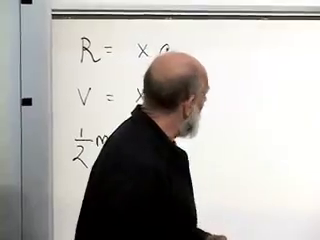
\includegraphics[width=0.72\textwidth]{lecture_09_figure_02.png}\caption{유클리드 공간 선요소에 척도인자가 곱해진 평탄 팽창 계량. 출처 프레임 00:09:12.}\label{fig:l09-expanding-metric-board}\end{figure}

고무판 위에 좌표를 그려 놓았다고 상상해 보자. 좌표 표지는 판에 붙어 그대로 있지만, 표지 사이의 물리적 거리는 커진다. 따라서 “\(x=0\)에서 \(x=1\)까지”와 같은 좌표 차이는 표지 두 개를 가리킬 뿐이다. 그 간격이 나타내는 거리는 \(a(t)\)이다. 이 척도인자를 지배하는 방정식을 찾는 것이 이번 강의의 동역학 문제다.

\section{닫힌 공간, 평탄한 공간, 열린 공간의 기하}

평탄성은 관측상의 단순화이지 균질성의 귀결은 아니다. 균질하고 등방적인 공간 기하는 곡률이 양수, 0, 음수인 세 가지다. 양의 곡률인 경우를 이해하려면 차원을 정확히 구분하는 것이 도움이 된다.

\begin{equation}
  X_1^2+X_2^2=R^2
\end{equation}의 자취는 원, 즉 일구 \(S^1\)다. 그 안을 채운 영역은 원판이며 이차원 공이라고도 한다. 매장 좌표를 하나 더하면 \begin{equation}
  X_1^2+X_2^2+X_3^2=R^2,
\end{equation}이 되고, 이는 보통의 이구 \(S^2\)다. 매장 좌표를 하나 더 추가하면 \begin{equation}
  X_1^2+X_2^2+X_3^2+X_4^2=R^2,
  \label{eq:l09-three-sphere}
\end{equation}이 되며, 이는 그 자체로 삼차원 공간인 삼구 \(S^3\)다. 우리는 그것이 매장된 4차원 공간을 그려 볼 수 없지만, 내재적 기하가 존재하는 데 그 매장은 필요하지 않다.

\begin{figure}[H]\centering
  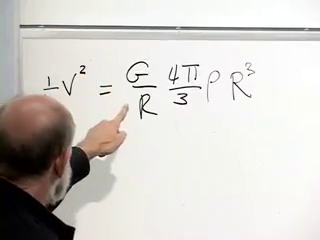
\includegraphics[width=0.72\textwidth]{lecture_09_figure_03.png}\caption{삼구를 소개할 때 사용한 매장 방정식. 출처 프레임 00:16:40.}\label{fig:l09-three-sphere-board}\end{figure}

이상적인 구의 모든 점은 기하학적으로 서로 동등하고, 한 점에서 모든 방향도 서로 동등하다. 따라서 구는 균질하면서 등방적이다. 반지름에 \(a(t)\)를 곱하면 구면 위에서 특정한 중심을 정하지 않고 공간 전체가 팽창하거나 수축한다. 이런 우주의 과거를 거슬러 올라가도 모든 물질이 외부의 빈 공간에 있는 한 특별한 지점에 모이는 것은 아니다. 공간 전체가 작아지므로 모든 점 쌍의 거리가 가까워진다. 빅뱅은 공간의 한 점에서 일어난 폭발이 아니다.

양의 곡률을 가진 구면에서 측지 삼각형의 내각의 합은 \(180^\circ\)보다 크다. 평탄한 삼각형의 내각의 합은 정확히 \(180^\circ\)이다. 안장으로 불완전하게 나타낼 수 있는 균질한 음의 곡률 기하에서는 내각의 합이 \(180^\circ\)보다 작다. 이러한 내재적 검사를 통해 세 경우를 구별할 수 있다.

\begin{figure}[H]\centering
  \includegraphics[width=0.72\textwidth]{lecture_09_figure_07.png}\caption{삼각형의 특징적인 모양으로 나타낸 양의 곡률, 영 곡률, 음의 곡률. 출처 프레임 00:37:30.}\label{fig:l09-curvature-board}\end{figure}

국소 계량이 완벽하게 평탄하다는 사실만으로 공간의 위상적 구조가 무한하다고 증명되지는 않는다. 콤팩트한 평탄 위상도 수학적으로 가능하지만, 이 강의에서는 가장 단순한 무한 유클리드 모형을 채택한다. \editorialnote{이러한 전역 위상에 관한 단서는 이후의 국소 동역학에는 필요하지 않다.}

\section{공변 좌표와 허블 법칙}

이제 팽창하는 평탄한 판으로 돌아가 그 위에 좌표 격자를 그려 보자. 공변 좌표계에서 격자는 큰 규모의 물질 흐름을 따라 함께 팽창한다. 은하, 또는 더 정확히는 충분히 거칠게 평균한 은하단은 물리적으로 다른 공변 물체와의 거리가 변하더라도 좌표 표지는 대체로 그대로 유지한다.

\begin{figure}[H]\centering
  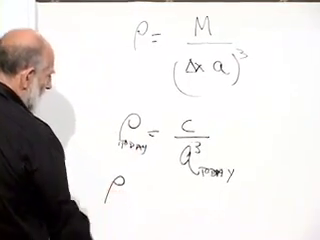
\includegraphics[width=0.72\textwidth]{lecture_09_figure_04.png}\caption{팽창하는 공간 판을 따라 움직이는 좌표 격자. 출처 프레임 00:22:20.}\label{fig:l09-comoving-grid-board}\end{figure}

\(x\)축을 따라 고정된 공변 간격 \(\Delta x\)만큼 떨어진 두 물체 사이의 물리적 거리는 다음과 같다. \begin{equation}
  D(t)=a(t)\,\Delta x.
  \label{eq:l09-physical-distance}
\end{equation}\(\Delta x\)을 고정한 채 미분하면 다음을 얻는다. \begin{equation}
  v(t)=\dot a(t)\,\Delta x
      =\frac{\dot a(t)}{a(t)}D(t).
\end{equation}다음과 같이 정의하면 \begin{equation}
  H(t)\equiv\frac{\dot a(t)}{a(t)},
  \label{eq:l09-hubble-parameter}
\end{equation}허블 법칙을 얻는다. \begin{equation}
  v=H(t)D.
  \label{eq:l09-hubble-law}
\end{equation}“허블 상수”에서 “상수”라는 말은 정해진 우주 시각에 공간 전체에서 일정하다는 뜻이다. 우주의 역사 전체에 걸쳐 일정하다는 뜻은 아니다.

\begin{figure}[H]\centering
  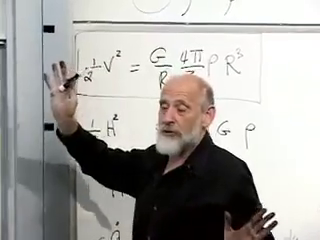
\includegraphics[width=0.72\textwidth]{lecture_09_figure_05.png}\caption{칠판 유도 \(D=a\Delta x\), \(v=(\dot a/a)D=HD\). 출처 프레임 00:26:40.}\label{fig:l09-hubble-board}\end{figure}

\begin{classroomqa}\audiencequestion{먼 은하를 더 이른 시기의 모습으로 관측했다면, 그곳에서 추론한 허블 매개변수도 오늘날 가까운 곳에서 측정한 값과 정말 같아야 할까요?}\lecturerresponse{되돌아보는 시간이 우주의 나이에 비해 짧을 때만 그렇습니다. 적당한 거리에서는 \(H(t)\)가 거의 변하지 않으므로 하나의 값으로 나타내도 충분합니다. 진정한 우주론적 거리를 관측할 때는 더 이른 시기의 우주를 보는 것이므로 \(a\)와 \(H\)의 시간 변화를 고려해야 합니다. 이것이 척도인자의 동역학 방정식이 필요한 이유 중 하나입니다.}\end{classroomqa}

\section{팽창 좌표계에서의 영광선}

\begin{classroomqa}\audiencequestion{척도인자는 먼 은하 사이를 전파하는 빛에도 영향을 줄까요?}\lecturerresponse{빛은 영 궤적을 따르므로 \(d\tau=0\)이다. 양의 \(x\)축을 따라 움직이는 광선에서는 \(dy=dz=0\)이고, 팽창 계량은 다음을 준다. \begin{align}
  0&=dt^2-a^2(t)dx^2,
  &dt&=a(t)dx,\notag\\
  &&\frac{dx}{dt}&=\frac{1}{a(t)}.
  \label{eq:l09-null-ray}
\end{align}\(a(t)\)가 커질수록 좌표 속도는 작아지지만, 국소적으로 측정하는 빛의 물리적 속도는 여전히 \(c=1\)이다. 고정된 좌표 간격이 나타내는 물리적 거리는 점점 커진다.}\end{classroomqa}

\begin{figure}[H]\centering
  \includegraphics[width=0.72\textwidth]{lecture_09_figure_06.png}\caption{방사형 빛 전파의 영 조건과 \(dt=a(t)dx\). 출처 프레임 00:30:54.}\label{fig:l09-null-board}\end{figure}

좌표를 선택하면 같은 사실을 “멀리 갈수록 빛이 느려진다”라고 표현할 수도 있지만, 그러면 길이와 시계에 대한 설명이 그에 따라 다루기 까다로워진다. 팽창하는 공간이라는 표현이 더 간결한 이유는 모든 자유낙하 관측자가 같은 빛의 속도를 측정한다는 국소적 진술을 그대로 보존하기 때문이다.

\begin{classroomqa}\audiencequestion{}먼 은하에서도 국소적인 빛의 전파와 원자 물리가 같다는 증거가 있나요?\lecturerresponse{무차원 비교만이 조작적으로 의미가 있다. 원자 크기를 길이의 단위로, 원자 또는 핵의 주기를 시간의 단위로 정한 다음, 빛이 그 길이를 가로지르는 데 그러한 주기가 몇 번 필요한지 물어보면 된다. 스펙트럼 관측은 이런 무차원비가 먼 영역에서도 같다는 진술을 뒷받침한다. 증거는 간접적이지만, 국소 법칙의 균일성을 검증하는 방법이 바로 이런 비교다.}\end{classroomqa}

관측 가능한 우주가 극도로 작았을 때는 그에 맞는 광행 시간 단위로 보면 빛이 일정한 물리적 영역을 빠르게 가로지를 수 있었다. 그렇다고 \(c\)가 달랐다는 뜻은 아니다. 영역 자체가 작았다는 뜻이다.

\section{우주 안의 뉴턴 구}

이제 운동학에서 동역학으로 넘어가자. 우리가 원점에 있다고 놓고, 많은 은하와 은하단을 포함할 만큼 큰 구를 그린다. 그 경계에 있는 은하 하나를 택한다. 균질한 우주에서는 질량 분포가 우리를 중심으로 구대칭이므로, 뉴턴의 껍질 정리에 따라 다음 두 가지 중요한 사실이 성립한다. \begin{enumerate}\item 선택한 반지름 바깥에 구형으로 분포한 모든 물질은 경계 은하에 순 뉴턴 힘을 전혀 가하지 않는다. \item 구 안에 있는 모든 물질은 이 방사 방향 운동에 대해 중심에 모여 있는 것처럼 작용한다. \end{enumerate}우리가 정지해 있는 기준계를 사용하므로, 다음 논증에서 속도와 가속도는 우리에 대한 값으로 측정한다.

\begin{figure}[H]\centering
  \includegraphics[width=0.72\textwidth]{lecture_09_figure_08.png}\caption{껍질 정리의 구성: 중심에 있는 우리와 균질한 큰 구의 경계에 놓인 시험 은하. 출처 프레임 00:41:10.}\label{fig:l09-shell-board}\end{figure}

\begin{figure}[H]\centering
  \begin{tikzpicture}[scale=0.92,>=Latex]
    \draw[thick] (0,0) circle (2.35);
    \fill (0,0) circle (2pt) node[below left] {us};
    \fill (2.35,0) circle (2.2pt) node[right] {test galaxy \(m\)};
    \draw[->,thick,blue!65!black] (0.18,0) -- (2.15,0)
      node[midway,above] {\(R=a(t)x\)};
    \draw[->,thick,red!65!black] (2.35,0.12) -- (3.25,0.12)
      node[midway,above] {\(v=\dot a(t)x\)};
    \node[align=center,text width=7cm] at (0,-2.85)
      {outside shells cancel;\\enclosed mass acts at the center};
  \end{tikzpicture}\caption{뉴턴 역학의 구성을 깔끔하게 다시 그린 그림.}\label{fig:l09-shell-clean}\end{figure}

은하의 공변 좌표 \(x\)가 고정되어 있다면, 물리적 반지름과 속도는 다음과 같다. \begin{equation}
  R(t)=x a(t),
  \qquad
  v(t)=x\dot a(t)=H(t)R(t).
  \label{eq:l09-radius-velocity}
\end{equation}구 안에 포함된 질량을 \(M\), 시험 은하의 질량을 \(m\)라 하자. 뉴턴 역학에서 에너지는 다음과 같다. \begin{equation}
  E=\frac12 m v^2-\frac{GMm}{R}.
  \label{eq:l09-newtonian-energy}
\end{equation}

\begin{figure}[H]\centering
  \includegraphics[width=0.72\textwidth]{lecture_09_figure_09.png}\caption{칠판의 전체 전개 \(R=xa\), \(v=x\dot a\) 및 \(E=0\)에 특화한 뉴턴 에너지 방정식. 출처 프레임 00:48:40.}\label{fig:l09-energy-board}\end{figure}

에너지는 양수, 0, 음수일 수 있다. 탈출과 재붕괴의 경계인 \(E=0\)인 경우부터 살펴보자. 이때는 다음과 같다. \begin{equation}
  \frac12 v^2=\frac{GM}{R}.
  \label{eq:l09-zero-energy}
\end{equation}

\begin{classroomqa}\audiencequestion{은 전체 에너지가 0이라는 것은 멀어지는 은하에 대해 어떤 뜻인가요?}\lecturerresponse{정확히 탈출 속도에 해당하는 경우다. 양의 에너지는 탈출 속도보다 빠른 운동을 뜻하고, 음의 에너지는 탈출 속도보다 느린 운동을 뜻하며, 물질만 있는 뉴턴 역학의 그림에서는 결국 되돌아온다. 우리는 이 두 가능성 사이의 경계에서 출발해 평탄 방정식을 유도한 다음 다른 부호의 경우를 살펴보겠다.}\end{classroomqa}

\begin{classroomqa}\audiencequestion{\(M\)구 안에 포함된 질량 }은 구가 팽창할 때 변하나요?\lecturerresponse{아니다. 구는 공변하므로 같은 입자들이 계속 그 안에 머문다. 물리적 부피는 커지고 밀도는 낮아지지만, 구 안에 포함된 전체 질량은 일정하게 유지된다. \(M\)과 \(\rho(t)\)의 차이를 구별하는 것이 중요하다.}\end{classroomqa}

균질한 밀도 \(\rho(t)\)에 대해 다음이 성립한다. \begin{equation}
  M=\frac{4\pi}{3}\rho(t)R^3.
  \label{eq:l09-enclosed-mass}
\end{equation}이를 \eqref{eq:l09-zero-energy}에 대입하면 다음을 얻는다. \begin{equation}
  \frac12 v^2
  =\frac{G}{R}\left(\frac{4\pi}{3}\rho R^3\right).
  \label{eq:l09-enclosed-energy}
\end{equation}

\begin{figure}[H]\centering
  \includegraphics[width=0.72\textwidth]{lecture_09_figure_10.png}\caption{영 에너지 방정식에 구 안의 질량을 대입한 모습. 출처 프레임 00:54:16.060.}\label{fig:l09-enclosed-mass-board}\end{figure}

\(v=HR\)를 사용하면 다음을 얻는다. \begin{align}
  \frac12 H^2R^2
    &=\frac{4\pi G}{3}\rho R^2,\\
  H^2
    &=\frac{8\pi G}{3}\rho.
\end{align}따라서 영 에너지, 공간 평탄 팽창 법칙은 다음과 같다. \begin{equation}
  \boxed{\left(\frac{\dot a}{a}\right)^2
  =\frac{8\pi G}{3}\rho(t)}.
  \label{eq:l09-flat-friedmann}
\end{equation}\(R^2\)의 소거는 우연이 아니다. 균질한 우주에서는 시험 물체로 어떤 공변 은하를 택하더라도 \(H(t)\)가 같아야 한다.

\begin{figure}[H]\centering
  \includegraphics[width=0.72\textwidth]{lecture_09_figure_11.png}\caption{칠판에 나타낸 반지름의 소거와 그 결과인 평탄 프리드만 관계식. 출처 프레임 00:57:30.}\label{fig:l09-friedmann-board}\end{figure}

\begin{classroomqa}
\audiencequestion{영에너지 관계를 뒷받침하는 증거가 있나요?}
\lecturerresponse{양변은 모두 관측을 통해 추론할 수 있습니다. \(H\)는 후퇴 자료에서, \(\rho\)는 별과 기체, 암흑 물질, 진공 에너지를 모두 고려해 구할 수 있습니다. 강의 당시의 비교에서는 두 양이 퍼센트 수준의 정확도로 일치하는 것으로 나타났습니다. 다만 중요한 조건이 있습니다. 모든 형태의 에너지를 포함해야 하며, 이후의 진공 에너지 논의에 따르면 단순한 탈출 속도 해석은 달라집니다.}
\end{classroomqa}

\(c=1\)인 단위계에서는 질량 밀도와 에너지 밀도의 단위가 같다. 따라서 기호 \(\rho\)는 논의 중인 성분에 해당하는 전체 에너지 밀도를 나타낸다.

\section{일반 물질과 2/3 법칙}

\eqref{eq:l09-flat-friedmann}만으로는 아직 방정식이 완결되지 않는다. \(\rho(t)\)가 어떻게 변하는지 알아야 한다. 먼저 천천히 움직이는 비상대론적 입자들로 공변 직육면체를 채워 보자. 상자의 좌표상 변 길이는 고정되어 있지만, 물리적 부피는 다음과 같이 커진다. \begin{equation}
  V(t)=a^3(t)\,\Delta x\,\Delta y\,\Delta z.
\end{equation}상자 안의 입자 수와 정지 질량은 그대로이므로 다음과 같다. \begin{equation}
  \rho_{\mathrm m}(t)=\frac{C_{\mathrm m}}{a^3(t)}.
  \label{eq:l09-matter-dilution}
\end{equation}현재 시각 \(t_0\)을 기준으로 정규화하면 다음과 같다. \begin{equation}
  \frac{\rho_{\mathrm m}(t)}{\rho_{\mathrm m,0}}
  =\left(\frac{a_0}{a(t)}\right)^3.
  \label{eq:l09-matter-normalized}
\end{equation}

\begin{figure}[H]\centering
  \includegraphics[width=0.72\textwidth]{lecture_09_figure_12.png}\caption{물질 밀도, 그 \(a^{-3}\) 희석, 현재 시점의 정규화. 출처 프레임 01:04:47.940.}\label{fig:l09-density-board}\end{figure}

\begin{classroomqa}\audiencequestion{}현재 우주의 대략적인 에너지 밀도는 얼마이며, 보통 원자만으로 이를 설명할 수 있나요?\lecturerresponse{눈에 보이는 중입자 물질만 세어서는 답의 일부만 얻는다. 암흑 물질과 암흑 에너지도 질량과 에너지의 등가물로 포함해야 한다. 강의에서는 정밀한 목록보다 규모를 강조하며, 에너지 밀도의 대략적인 범위를 수소 원자 질량으로 환산한 입자 하나에서 수십 개 정도의 세제곱미터당 값으로 제시한다.}\end{classroomqa}

\eqref{eq:l09-matter-dilution}를 \eqref{eq:l09-flat-friedmann}에 대입하고 시간에 무관한 인자들을 모두 양의 상수 \(C\)에 포함시키면 다음을 얻는다. \begin{equation}
  \left(\frac{\dot a}{a}\right)^2=\frac{C}{a^3},
  \qquad
  \dot a^2=\frac{C}{a}.
  \label{eq:l09-matter-ode}
\end{equation}방정식을 푸는 방법은 명료하게 두 가지다. 멱법칙 해 \(a=K t^p\)를 가정하면 다음 조건이 필요하다. \begin{equation}
  p-1=-\frac{p}{2},
  \qquad p=\frac23.
\end{equation}같은 방정식에서 팽창에 해당하는 제곱근 가지를 택해 적분할 수도 있다. \begin{equation}
  a^{1/2}\frac{da}{dt}=\sqrt C,
  \qquad
  \int a^{1/2}da=\sqrt C\int dt,
\end{equation}따라서 빅뱅을 시간의 원점으로 택하면 다음과 같다. \begin{equation}
  a^{3/2}\propto t,
  \qquad
  \boxed{a(t)\propto t^{2/3}}.
  \label{eq:l09-matter-solution}
\end{equation}실시간 칠판 유도에서는 계수를 맞추는 과정에서 인자 하나가 잠시 빠졌지만, 적분으로 돌아가 지수를 확인했다. 이 노트에는 그 확인 과정을 유지하되, 수정된 대수식만 제시한다.

\begin{figure}[H]\centering
  \includegraphics[width=0.72\textwidth]{lecture_09_figure_13.png}\caption{멱법칙 가정과 상자 안에 표시한 지수 \(p=2/3\). 출처 프레임 01:13:05.}\label{fig:l09-matter-solution-board}\end{figure}

해를 미분하면 다음을 얻는다. \begin{equation}
  H(t)=\frac{\dot a}{a}=\frac{2}{3t}.
  \label{eq:l09-matter-hubble}
\end{equation}과거에는 허블 매개변수가 더 컸다. 따라서 되돌아보는 시간이 상당히 길 정도로 먼 곳을 볼 때는 오늘날의 \(H_0\)를 그대로 써서 국소적 선형 관계를 연장해서는 안 된다.

\begin{figure}[H]\centering
  \includegraphics[width=0.72\textwidth]{lecture_09_figure_14.png}\caption{\(\dot a/a\)에 \(a\propto t^{2/3}\)를 대입하면 다음을 얻는다. \(H=2/(3t)\). 출처 프레임 01:20:42.}\label{fig:l09-hubble-time-board}\end{figure}

\section{에너지 부호와 공간 곡률}

뉴턴 역학의 논증으로 영 에너지인 평탄한 경우까지 유도했다. 일반 상대성 이론에는 껍질 정리만으로는 얻을 수 없는 사실이 하나 더 있다. 뉴턴식 비에너지의 부호는 공간 곡률의 부호에 대응한다.
\begin{center}\begin{tabular}{@{}>{\raggedright\arraybackslash}p{0.20\linewidth}
                    >{\raggedright\arraybackslash}p{0.29\linewidth}
                    >{\raggedright\arraybackslash}p{0.37\linewidth}@{}}\toprule
  전체 에너지&공간 곡률&물질만 있을 때의 운명\\
\midrule
  양수&음수(열린 우주)&영원히 팽창\\
0&0(평탄한 우주)&탈출 경계에 가까워진다\\
음수&양수(닫힌 우주)&팽창하다가 방향을 바꾸어 재붕괴한다\\
\bottomrule
\end{tabular}\end{center}마지막 열은 진공 에너지가 없다고 가정한다. 발사체의 비유에서 양의 에너지는 탈출 속도보다 빠른 경우, 0은 정확히 탈출 속도인 경우, 음의 에너지는 탈출 속도보다 느린 경우를 뜻한다. 아인슈타인 방정식은 이 세 경우를 각각 열린 공간, 평탄한 공간, 닫힌 공간 기하와 연결한다.

\section{광자와 1/2 법칙}

물질 법칙 \(\rho\propto a^{-3}\)은 입자 수밀도가 낮아지는 동안 각 입자의 에너지는 대략 일정하다고 가정한다. 광자는 이 가정을 따르지 않는다. 광자의 경우 \begin{equation}
  E=h\nu=\frac{hc}{\lambda}.
\end{equation}팽창하면 파장이 척도인자에 비례해 늘어난다. \begin{equation}
  \lambda\propto a,
  \qquad E\propto a^{-1}.
\end{equation}광자 수밀도는 여전히 \(a^{-3}\)에 따라 낮아지며, 각 광자의 에너지에도 \(a^{-1}\)라는 인자가 하나 더 들어간다. 따라서 다음과 같다. \begin{equation}
  \boxed{\rho_{\mathrm r}(t)\propto a^{-4}(t)}.
  \label{eq:l09-radiation-dilution}
\end{equation}

기타 줄의 비유는 물리적 상황을 잘 보여 준다. 줄을 튕긴 뒤 진동하는 부분을 길게 늘이면 파장이 늘고 음높이가 낮아진다. 팽창하는 공변 상자 안의 광자 모드도 비슷하게 거동한다. 이 상황을 거꾸로 보면 압축 시 파장이 짧아지고 광자 에너지가 커진다.

\begin{figure}[H]\centering
  \includegraphics[width=0.72\textwidth]{lecture_09_figure_15.png}\caption{칠판에서 물질 밀도 관계식을 복사 밀도 스케일링 \(\rho_{\mathrm r}\propto a^{-4}\)까지 확장한 모습. 출처 프레임 01:29:20.}\label{fig:l09-radiation-board}\end{figure}

\(\rho_{\mathrm r}\propto a^{-4}\)를 평탄 프리드만 방정식에 대입하면 다음과 같다. \begin{equation}
  \left(\frac{\dot a}{a}\right)^2=\frac{C_{\mathrm r}}{a^4},
  \qquad
  \dot a\propto a^{-1},
\end{equation}그러므로 다음을 얻는다. \begin{equation}
  \boxed{a(t)\propto t^{1/2}}.
  \label{eq:l09-radiation-solution}
\end{equation}이는 \(t^{2/3}\)보다 느리게 증가한다. 충분히 과거로 거슬러 올라가면 \(a^{-4}\)가 \(a\)가 감소할수록 \(a^{-3}\)보다 더 빠르게 커지므로 복사가 보통 물질보다 우세해진다. 강의에서는 척도인자가 오늘날보다 대략 천 배 작았던 시기를 물질과 복사의 교차 시점으로 잡는다. 그보다 앞선 우주는 복사가 지배했고, 그 이후에는 오랜 기간 물질이 지배했다.

\section{진공 에너지와 지수 팽창}

진공 에너지는 정반대의 스케일링 거동을 보인다. 진공 에너지의 밀도는 빈 공간의 성질이므로 우주가 팽창해도 희석되지 않는다. \begin{equation}
  \rho_\Lambda=\text{constant}.
  \label{eq:l09-vacuum-density}
\end{equation}보통 물질과 복사는 과거로 갈수록 밀도가 높아지지만, 이 항은 그렇지 않다. 따라서 초기 우주에서는 영향이 작았고, 다른 성분들이 희석됨에 따라 점점 중요해진다. 강의에서는 당시 추정치에 따라 진공 에너지가 오늘날 우주 에너지 밀도의 약 \(70\%\)를 차지한다고 본다.

\(\rho_\Lambda\)가 일정하면 방정식 \eqref{eq:l09-flat-friedmann}에서 팽창률도 일정해진다. \begin{equation}
  H_\Lambda=\sqrt{\frac{8\pi G}{3}\rho_\Lambda},
  \qquad
  \frac{\dot a}{a}=H_\Lambda.
\end{equation}따라서 다음과 같다. \begin{equation}
  \boxed{a(t)=a(t_i)e^{H_\Lambda(t-t_i)}}.
  \label{eq:l09-vacuum-solution}
\end{equation}

\begin{figure}[H]\centering
  \includegraphics[width=0.72\textwidth]{lecture_09_figure_16.png}\caption{지수 팽창으로 이어지는 일정한 밀도 방정식. 출처 프레임 01:35:48.}\label{fig:l09-vacuum-board}\end{figure}

강의에서 언급한 관측 규모에서는 우주의 선형 크기가 대략 백억 년에서 백이십억 년에 걸쳐 두 배가 됩니다. 이 작지만 0이 아닌 진공 밀도의 기원은 여전히 설명되지 않았습니다. 그것의 존재와 팽창에 미치는 영향은 관측으로 확인된 사실입니다.

\begin{classroomqa}\audiencequestion{}이 논의에서 진공 에너지는 암흑 에너지와 같은 것인가요?\lecturerresponse{그렇다. 여기서 “암흑 에너지”는 일정한 진공 에너지 밀도, 즉 우주 상수를 뜻한다. 시간에 따라 변하는 더 일반적인 암흑 에너지 모형도 상정할 수 있지만, 이 강의의 계산에서는 다루지 않는다.}\end{classroomqa}

\section{팽창 우주가 빛을 적색편이시키는 방식}

\begin{classroomqa}\audiencequestion{우리가 팽창하는 공변 좌표를 택했다는 이유만으로 광자가 어떻게 그 사실을 알아차리고 에너지를 낮추나요?}\lecturerresponse{광자는 우리의 좌표 표지에 반응하지 않는다. 물리적 거리 간격이 변하는 기하를 따라 전파된다. 물리적 크기가 두 배가 되는 영역을 차지한 파동열은 파장도 두 배가 된다. 공변 좌표는 이러한 늘어남을 간결하게 기술할 뿐, 그 원인은 아니다.}\end{classroomqa}

\begin{classroomqa}\audiencequestion{오늘날 우리에게 도달하는 배경 광자는 어디에서 오는 건가요?}\lecturerresponse{더 먼 곳을 본다는 것은 더 이른 시기를 본다는 뜻이다. 더 거슬러 가면 우주의 물질이 이온화된 플라스마였던 시기를 보게 된다. 이때 광자는 자유 전하 입자에 반복해서 산란되어 우주가 불투명했다. 광자가 마지막으로 자유롭게 출발해 우리에게 올 수 있었던 경계는 관측자를 둘러싼 구면으로 보인다. 이것이 마지막 산란면이다.}\end{classroomqa}

\begin{figure}[H]\centering
  \includegraphics[width=0.72\textwidth]{lecture_09_figure_17.png}\caption{관측자를 중심으로 마지막 산란면과 점점 멀어지는 껍질을 그린 그림. 출처 프레임 01:42:05.}\label{fig:l09-last-scattering-board}\end{figure}

\begin{figure}[H]\centering
  \begin{tikzpicture}[scale=0.9,>=Latex]
    \fill (0,0) circle (2pt) node[below] {observer};
    \draw[thick,orange!70!black] (0,0) circle (2.55);
    \node[orange!70!black,align=center] at (0,3.05)
      {surface of last scattering};
    \foreach \a in {25,75,145,210,285,335}{
      \draw[->,blue!60!black] ({2.55*cos(\a)},{2.55*sin(\a)}) --
        ({1.7*cos(\a)},{1.7*sin(\a)});
    }
    \draw[decorate,decoration={snake,amplitude=1.5pt,segment length=7pt},
      red!65!black,thick,->] (-2.5,0) -- (-0.15,0);
    \node[red!65!black,below] at (-1.35,-0.15)
      {redshifted photon};
  \end{tikzpicture}\caption{마지막 산란 그림을 깔끔하게 다시 그린 모습.}\label{fig:l09-last-scattering-clean}\end{figure}

복사는 뜨거운 플라스마의 특징적인 스펙트럼을 띠고 방출되었으며, 파장이 대략 천 배 길어져 우리에게 도달한다. 강의의 도플러 표현을 따르면, 먼 방출면은 빠르게 멀어지고 그 복사는 크게 적색편이된다. 기하학적 표현을 따르면, 전파 중에 파동이 늘어난다. 두 관점은 같은 관계를 나타낸다. \begin{equation}
  1+z=\frac{\lambda_0}{\lambda_{\mathrm{em}}}
      =\frac{a_0}{a_{\mathrm{em}}}.
  \label{eq:l09-cosmological-redshift}
\end{equation}\editorialnote{방정식 \eqref{eq:l09-cosmological-redshift}은 파동의 늘어남과 도플러 효과라는 강의의 설명을 표준적인 정량식으로 나타낸 것이다.}

더 이른 시기에 관측한다면 그에 대응하는 그림에서 마지막 산란면은 더 가까이 있을 것이며, 관측되는 배경 광자는 적색편이가 덜 되어 에너지가 더 높을 것이다. 우주 시간이 흐를수록, 초기 플라스마에서 출발해 공변 관측자에게 도달하는 광자의 파장은 점점 길어진다.

\section{적색편이된 광자의 에너지는 어디로 가는가?}

\begin{classroomqa}\audiencequestion{광자가 \(h\nu_{\mathrm{em}}\)의 에너지를 지닌 채 방출되었다가 적색편이를 거쳐 더 낮은 에너지로 도달합니다. 그 차이는 어떻게 된 건가요?}\lecturerresponse{뉴턴 역학의 유도는 에너지 방정식에서 출발했다. 그 우주론적 형태는 팽창률과 물질 에너지 밀도를 연결하므로, 물질 에너지와 팽창을 서로 독립적으로 보존되는 양처럼 다룰 수 없다. 강의에서는 광자가 잃은 에너지가 팽창의 운동에너지 장부에 들어간다고 설명한다. 복사를 채운 피스톤은 이 비유를 구체적으로 보여 준다. 복사 압력이 피스톤을 바깥쪽으로 밀면 광자의 파장이 길어지고 에너지는 낮아지며, 잃은 에너지는 피스톤의 기계적 일과 운동에너지가 된다.}\end{classroomqa}

\begin{figure}[H]\centering
  \includegraphics[width=0.72\textwidth]{lecture_09_figure_18.png}\caption{칠판에 상자 표시한 뉴턴 에너지 방정식과 그에 대응하는 프리드만 방정식이 위아래로 놓여 있다. 출처 프레임 01:44:42.}\label{fig:l09-energy-bookkeeping-board}\end{figure}

\begin{classroomqa}\audiencequestion{}복사 에너지는 무엇을 통해 팽창과 결합하나요?\lecturerresponse{압력이다. 움직이는 피스톤이 달린 원통에서는 광자가 벽에 운동량을 전달한다. 피스톤이 움직이면 복사가 일을 하고, 파장은 길어지며 에너지는 낮아진다. 균질하게 팽창하는 우주에는 실제 바깥 피스톤이 없지만, \(p\,dV\) 비유를 통해 복사 에너지 밀도가 입자 수 희석만으로 예상하는 것보다 더 빠르게 감소하는 이유를 이해할 수 있다.}\end{classroomqa}

\begin{figure}[H]\centering
  \includegraphics[width=0.72\textwidth]{lecture_09_figure_19.png}\caption{압력이 하는 일을 시각화하는 데 사용한, 움직이는 피스톤이 달린 광자 충전 용기. 출처 프레임 01:46:40.}\label{fig:l09-piston-board}\end{figure}

\begin{figure}[H]\centering
  \begin{tikzpicture}[scale=0.92,>=Latex]
    \draw[thick] (0,0) rectangle (5.3,2.6);
    \draw[very thick] (4.25,0) -- (4.25,2.6);
    \draw[very thick] (4.25,1.3) -- (5.25,1.3);
    \draw[->,thick,red!65!black] (5.25,1.3) -- (6.2,1.3)
      node[right] {moving piston};
    \foreach \y in {0.55,1.3,2.05}{
      \draw[decorate,decoration={snake,amplitude=1.4pt,segment length=6pt},
        blue!65!black,->] (0.35,\y) -- (3.9,\y);
    }
    \node at (2.15,-0.45) {radiation does \(p\,dV\) work};
  \end{tikzpicture}\caption{복사와 피스톤의 비유를 깔끔하게 다시 그린 그림.}\label{fig:l09-piston-clean}\end{figure}

일반상대론에서 에너지를 논할 때는 주의가 필요하다. 일반적인 팽창 시공간에서는 고립된 뉴턴계의 에너지와 같은 유일한 보존 전역 에너지가 존재하지 않을 수 있다. 국소적인 응력-에너지 보존은 여전히 성립하며, 균질한 유체의 경우 연속 방정식으로 이어진다.
\begin{equation}
  \dot\rho+3H(\rho+p)=0,
  \label{eq:l09-continuity}
\end{equation}
이 식에는 물질과 복사의 스케일링 법칙을 낳는 압력에 의한 일이 포함되어 있다.\editorialnote{식 \eqref{eq:l09-continuity}은 강의에서 의도적으로 뉴턴역학의 에너지 장부 정리에 비유한 내용의 바탕이 되는, 정확한 국소 일반상대론적 진술이다.}

진공 에너지를 고려하면 이 문제는 특히 선명해진다. 진공 에너지 밀도는 일정하게 유지되는 반면 부피는 커지므로, 공변 영역 안의 진공 에너지 총량은 증가한다. 음의 압력은 중력의 원천에 포함되며 가속 팽창을 일으킨다. 따라서 기하와 압력에 의한 일을 포함하지 않은 채, 순진하게 생각한 ‘공변 상자 안의 물질 에너지’가 따로 보존되어야 한다고 요구해서는 안 된다.

\section{시간 항에서 스케일 인자를 없앨 수 있는 이유}

\begin{classroomqa}
\audiencequestion{계량의 공간 부분에는 스케일 인자가 곱해지는데 시간 부분에는 곱해지지 않는 이유는 무엇인가요?}
\lecturerresponse{그것은 시간 좌표를 어떻게 선택하느냐의 문제입니다. 등각시간 좌표 \(t\)에서 다음과 같이 시작한다고 합시다.
\begin{equation}
  d\tau^2=A^2(t)\left(dt^2-dx^2\right).
\end{equation}
새로운 우주시간 \(T\)을 다음과 같이 정의하면
\begin{equation}
  dT=A(t)\,dt.
\end{equation}
다음과 같이 됩니다.
\begin{equation}
  d\tau^2=dT^2-A^2\bigl(t(T)\bigr)dx^2.
\end{equation}
시간 미분 앞의 공통 인자는 사라지고, 공간 항에는 물리적 스케일 인자가 그대로 남습니다.}
\end{classroomqa}

\begin{figure}[H]
  \centering
  \includegraphics[width=0.72\textwidth]{lecture_09_figure_20.png}
  \caption{등각시간을 우주시간으로 변환하는 시간 재정의 \(dT=A(t)dt\). 원본 영상 프레임 01:5105}
  \label{fig:l09-time-reparam-board}
\end{figure}

\section{곡률, 진공 에너지, 우주의 운명}

\begin{classroomqa}
\audiencequestion{우주가 양의 곡률을 가진다면, 우리는 벌써 은하들이 우리 쪽으로 다가오는 것을 보고 있어야 하지 않나요?}
\lecturerresponse{반드시 그렇지는 않습니다. 탈출 속도보다 낮은 속도로 발사된 물체는 먼저 바깥쪽으로 움직이다가 방향 전환점에 이른 뒤에야 되돌아옵니다. 우리는 우주가 팽창하는 시기에 우주를 관측하고 있습니다. 진공 에너지가 없다면 양의 곡률을 가진 물질 우주는 결국 다시 수축하게 됩니다. 충분히 큰 양의 진공 에너지는 그런 방향 전환을 막으며, 관측된 값은 공간 곡률이 조금 있더라도 장기적으로 팽창이 지수적으로 이루어질 만큼 큰 것으로 보입니다.}
\end{classroomqa}

지수적으로 팽창하는 미래가 에너지의 낙원인 것은 아니다. 별들은 결국 연료를 다 태우고, 물질과 복사의 밀도는 지수적으로 낮아지며, 멀리 떨어진 영역들은 인과적으로 서로 접촉할 수 있는 범위를 벗어난다. 진공 에너지는 남아 있는 반면, 보통의 구조는 점점 더 차갑고 희박해진다.

\begin{classroomqa}
\audiencequestion{과거로 더 거슬러 올라가면 보통의 입자보다 광자가 더 많나요?}
\lecturerresponse{광자 수와 바리온 수의 비는 이미 매우 커서, 강의에서 추산한 값으로 바리온 하나당 광자 \(10^{10}\)개 정도이며, 공변 부피 안의 두 수는 모두 거의 일정하게 유지됩니다. 과거로 갈수록 주로 달라지는 것은 광자 하나당 에너지입니다. 광자 에너지는 \(a^{-1}\)에 따라 증가하지만, 비상대론적 정지 질량은 그렇지 않습니다. 따라서 수의 비 자체는 달라지지 않아도 초기 우주에서는 복사가 에너지 밀도를 지배합니다.}
\end{classroomqa}

핵심은 기하만으로 우주의 역사가 정해지지는 않는다는 점입니다. 평탄한 프리드만 방정식은 팽창과 에너지 밀도 사이의 관계를 제시하지만, 시간에 따른 변화는 우주를 이루는 물질과 에너지가 결정합니다. 비상대론적 물질에서는 \(a\propto t^{2/3}\), 복사에서는 \(a\propto t^{1/2}\)이며, 일정한 진공 에너지는 지수 팽창을 일으킵니다. 이 세 법칙은 우주의 연속적인 시대들을 정리해 주며, 같은 스케일 인자가 거리와 적색편이, 허블 매개변수의 변화를 어떻게 좌우하는지 설명합니다.

\end{document}